\documentclass[a4paper,fleqn,usenatbib]{mnras}
%=========================================================================
\usepackage{amsmath}
\usepackage{amssymb}
\usepackage{graphicx}
\usepackage{grffile}
\usepackage{float}
\usepackage[dvips]{epsfig}
\usepackage{epsfig}
\usepackage{dblfloatfix}
\usepackage{color}
\usepackage{caption}
\usepackage{hyperref}
\usepackage{bm}
%Non reposionated tables
\newcommand{\HI}{{\text{H\MakeUppercase{\romannumeral 1}}} }
\newcommand{\lya}{\ifmmode{{\rm Ly}\alpha}\else Ly$\alpha$\ \fi}
\newcommand{\kms}{\ifmmode\mathrm{km\ s}^{-1}\else km s$^{-1}$\fi}
\newcommand{\vrot}{\ifmmode v_{\mathrm{rot}}\else $v_{\mathrm{rot}}$~\fi}
\newcommand{\vout}{\ifmmode v_{\mathrm{out}}\else $v_{\mathrm{out}}$~\fi}
\newcommand{\tauh}{\ifmmode \tau_{\mathrm{H}}\else $\tau_{\mathrm{H}}$~\fi}
\newcommand{\vth}{\ifmmode v_{\mathrm{th}}\else $v_{\mathrm{th}}$~\fi}

\begin{document}

%=========================================================================
%		FRONT MATTER
%=========================================================================
\title[Outflows and rotation in LAEs]{Lyman-$\alpha$ photons through rotating outflows}
\author[M.C. Remolina-Gutierrez \& J.E. Forero-Romero]{
  Maria Camila Remolina-Guti\'errez$^{1}$
  \thanks{mc.remolina197@uniandes.edu.co} \&
  Jaime E. Forero-Romero $^{1}$
  \thanks{je.forero@uniandes.edu.co}\\
  %%
  $^{1}$ Departamento de F\'isica, Universidad de los Andes, Cra. 1
  No. 18A-10 Edificio Ip, CP 111711, Bogot\'a, Colombia \\
}

\maketitle

\begin{abstract}
Outflows and rotation are two ubiquitous kinematic features in the gas
kinematics of galaxies.
Here we perform Monte Carlo radiative transfer simulations of outflowing
gas with additional solid body rotation to understand how these kinematic
features impact the morphology of the Lyman-$\alpha$ emission line.
We explore a range of Hydrogen optical depth of
$10^5\leq\tauh\leq10^7$, rotational velocity $0\leq \vrot/\kms \leq 100$ and
outflow velocity $0\leq \vout/\kms\leq 50$.  
We find three important consequences of rotation.
First, it introduces a dependency with viewing angle; second it
produces a line broadening and third it increases the flux at the
line's center.
We also develp a semi-analytic model that modifies the spectra of
pure outflow simulations and manages to reproduce the line widths
and flux change at the line's center within a $7\%$ and $50\%$
precision, respectively.
\end{abstract}

\begin{keywords}
radiative transfer --- Methods: numerical
\end{keywords}


%=========================================================================
%		PAPER CONTENT
%=========================================================================

%*************************************************************************

\section{Introduction}
\label{sec:intro}

Recent advances in instrumentation have revealed the presence of gas
rotation on vastly different physical scales.
For instance, spatially resolved spectra on compact dwarf galaxies
have measured clear signs of gas showing pure rotation kinematics
\citep{2015A&A...577A..21C,2017A&A...600A.125C} and the recent mapping of
high redshift circumgalactic regions have also revealed kinematic
evidence for large scale rotation \citep{2018MNRAS.473.3907A}.
These systems with star formation, neutral gas and low dust
contents naturally show a \lya emission line \citep{PartridgePeebles}
motivating the observational work to phenomenologically link
H$\alpha$ kinematics to \lya spectra \citep[e.g.][]{Herenz2016}. 


What is then the expected imprint of rotation on a resonant emission
line such as the \lya line? To what extent is possible to constrain
rotational kinematics from the \lya emission line? 
Detailed radiative transfer (RT) \lya modeling of rotating systems
started until recently by \cite{Garavito14}.
In that work the authors studied the influence of pure solid body
rotation on the \lya line's morphology.
They found that rotation indeed introduces changes, the most
noticeable being the dependence of the spectra with the viewing
angle with respect to the rotation axis. 

\cite{Garavito14} also presented a simple semi-analytical
approximation that accounted for the main features of the \lya spectra
from a rotation sphere.
Recently, this semi-analytic solution was used to perform a Markov
Chain Monte Carlo exploration to fit the observed spectra Compact
Dwarf Galaxy \citep{tololo} with atypical features that could be
explained by pure rotation.  

However, the gas dynamics in Lyman Alpha Emitter (LAE) galaxies is
more complex than pure rotation.
The case for outflows as traced in the \lya line is much better
stablished.
In many observations the \lya line profiles has a single peak
redwards from the line's center, in other cases there is a double peak
but the peak on the red side is stronger
\citep[e.g.][]{2010ApJ...717..289S,Erb14,Trainor16}.   
These features been readily explained as the consequence of multiple
\lya photon scatterings through an homogeneous outflowing shell of
neutral Hydrogen
\citep{2006A&A...460..397V,Orsi12,2012ApJ...751...29Y,2015ApJ...812..123G}.  

An study of the combined effects of outflows and rotation has not been
presented in the literature.
Here we present such a study. 
We investigate a simplified geometrical configuration corresponding to a
spherical gas cloud with symmetrical radial outflows and solid body
rotation. 
We base our modeling on a Monte-Carlo radiative transfer code.
Besides modeling the impact of joint rotation and outflows, we also
check to what extent the analytical model presented by
\cite{Garavito14} to explain the effects of rotation can also be
applied in our case.

The structure of the paper is the following.
We introduce first our theoretical tools and assumptions
in Section \ref{sec:theory}. We continue in Section  \ref{sec:results}
with the results from the Monte-Carlo simulation, the comparison
against the semi-analytical approximation which we use to make a
thorough exploration of the effect of rotation.
In Section \ref{sec:discussion} we discuss our results and their
possible implications for observational analysis to finally present
our conclusions in Section \ref{sec:conclusions}.




\begin{figure*}
\centering
    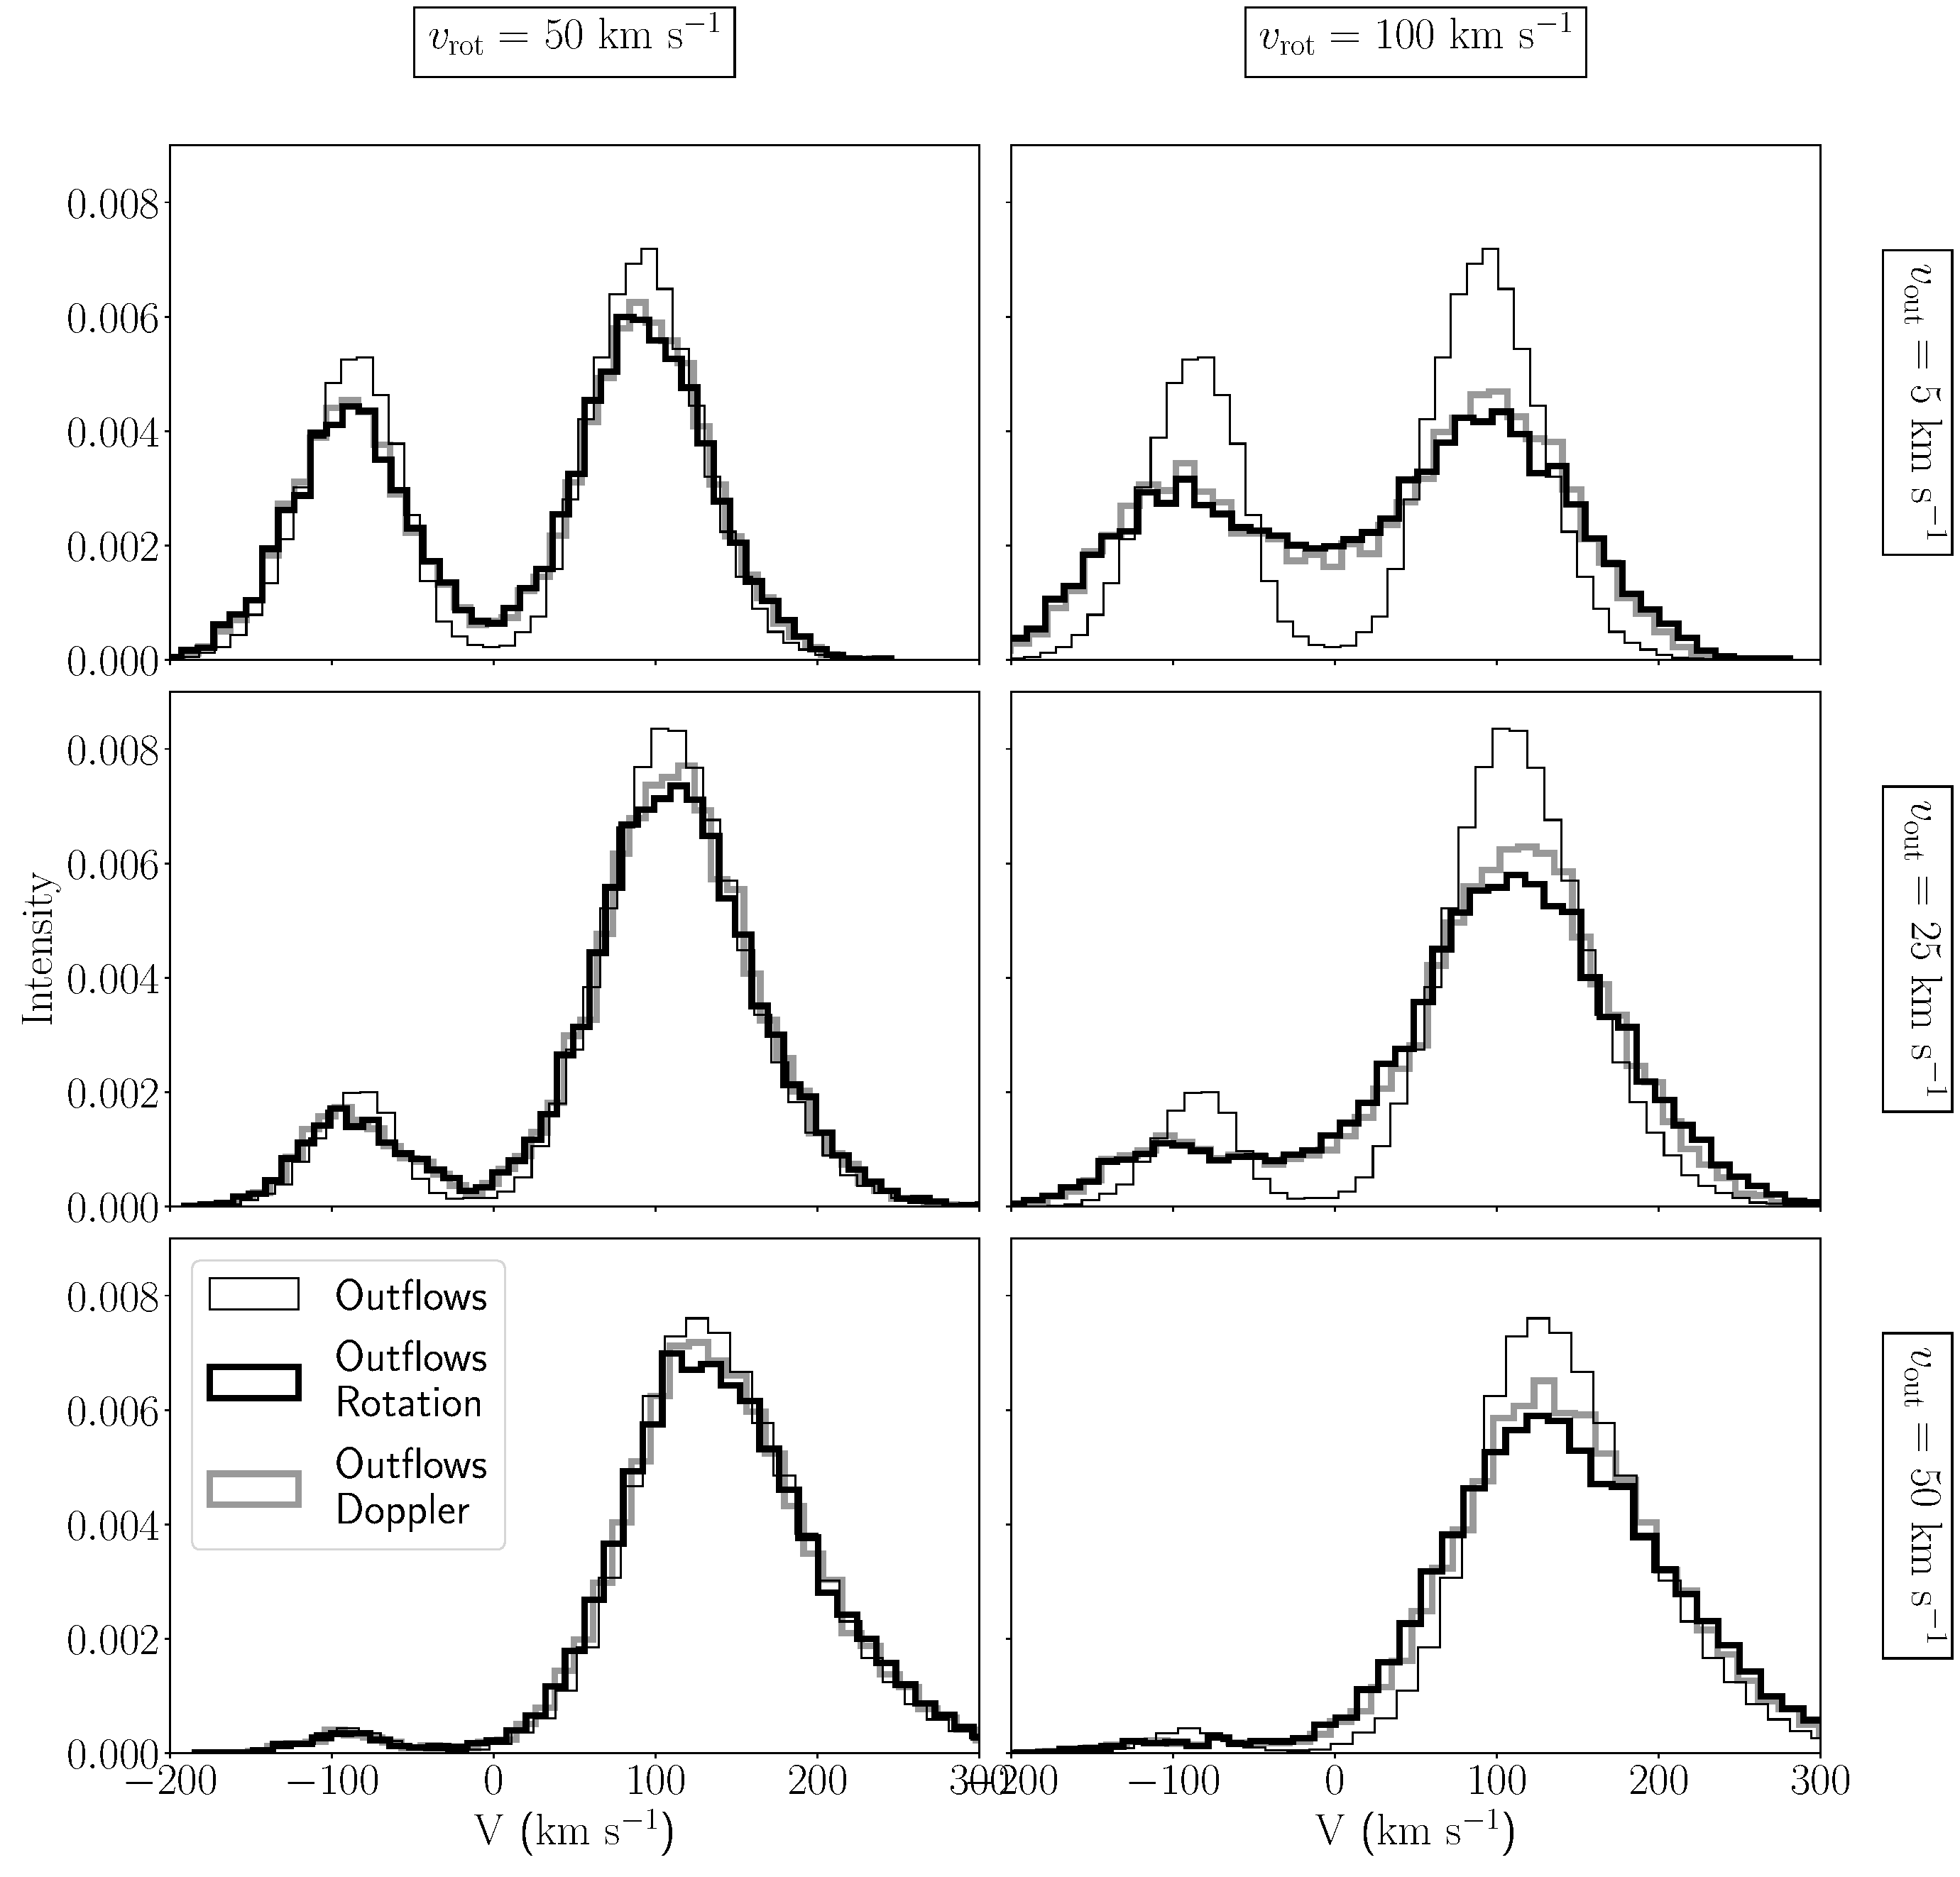
\includegraphics[width=0.48\textwidth]{./figures/results/doppler_shift_logtau6_theta90}
    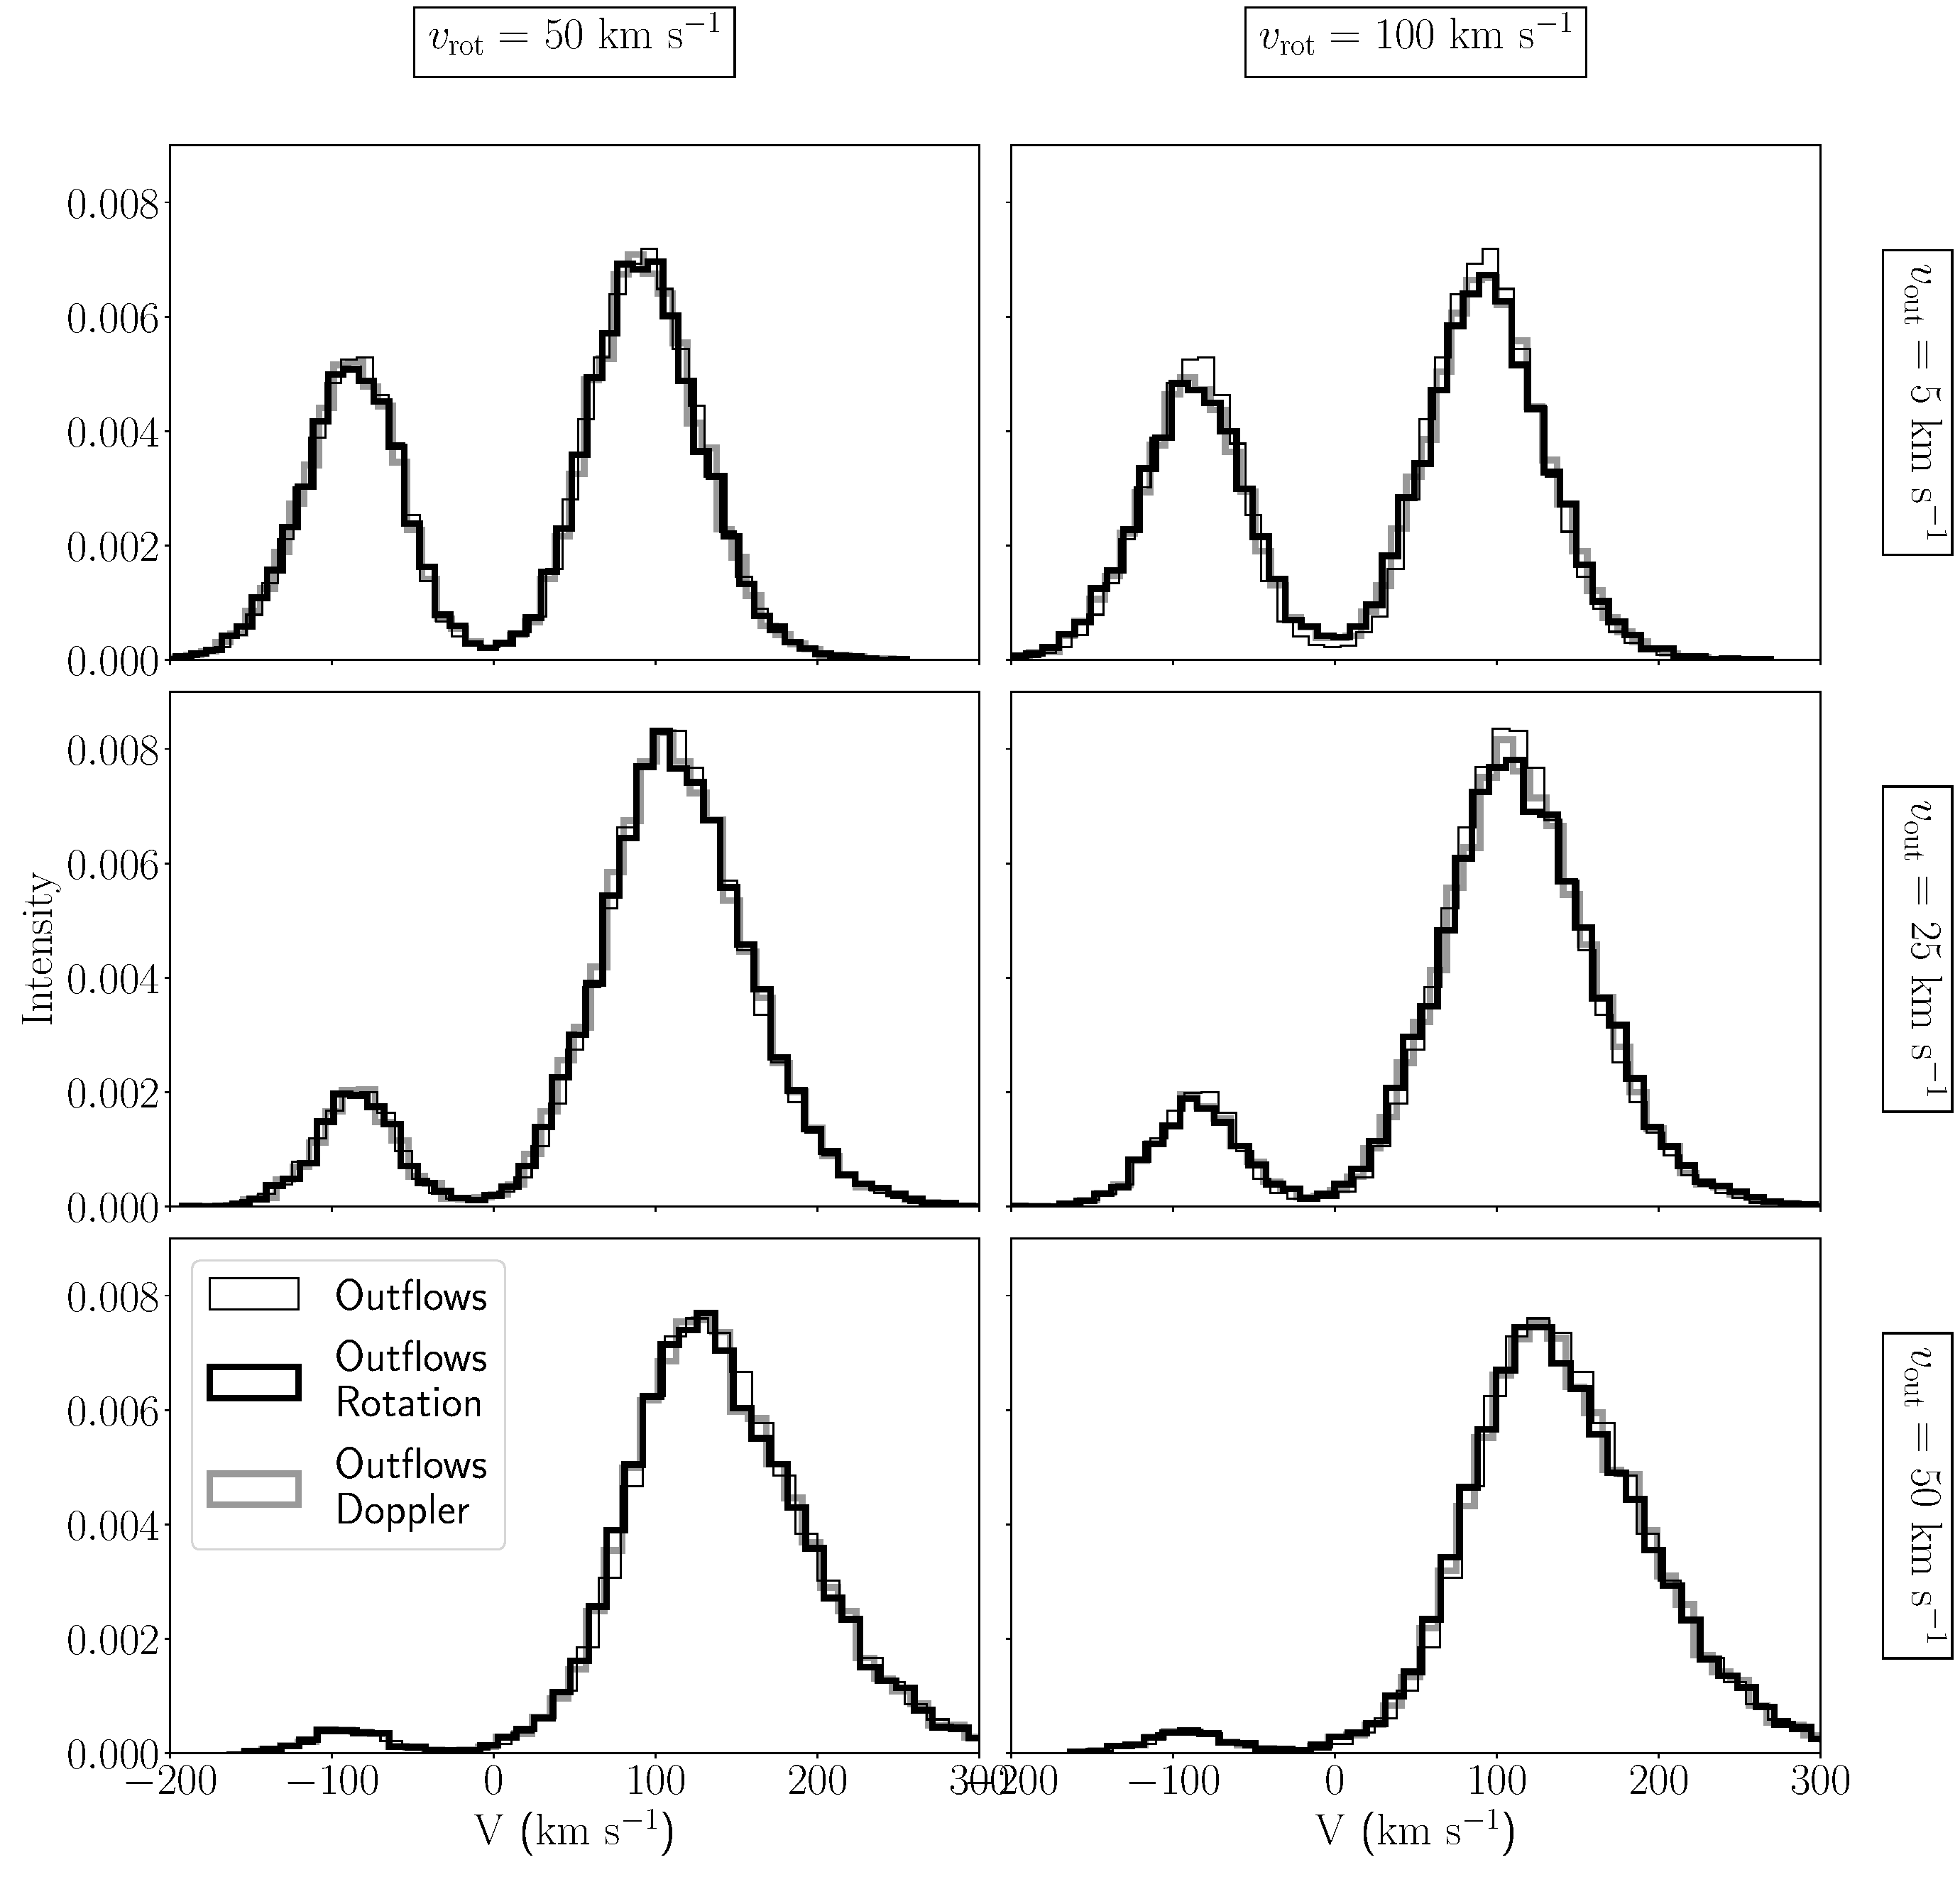
\includegraphics[width=0.48\textwidth]{./figures/results/doppler_shift_logtau6_theta0}
  \caption{\textbf{Qualitative trends of changing outflow and
      rotational velocity viewed perpendicular/paralell to the
      rotation axis}.  
    Here we fix $\tauh=10^6$. 
    The six panels on the left correspond to $\theta=90^\circ$ and the
    panels on the right to $\theta=0^{\circ}$
    We vary \vrot increasing from left to right and \vout increasing
    from top to bottom. 
    The thin black line corresponds to the \lya line obtained with
    CLARA without any rotation and the indicated outflow velocity.
    The thick black line corresponds to the results including both
    outflows and rotation.
    The thick gray line shows the results of modifyin the pure outflow
    solution by the Doppler shift presented in Equation \ref{eq:shift_x}
    (in thin line), if there is a radiative transfer of rotation and outflows
    (thick and clear line), and if there is a radiative transfer of
    only outflows, but also a Doppler shift from the rotational
    velocity (thick and dark line).  
    \label{fig:doppler_shift}}
\end{figure*}




\begin{figure*}
\begin{center}
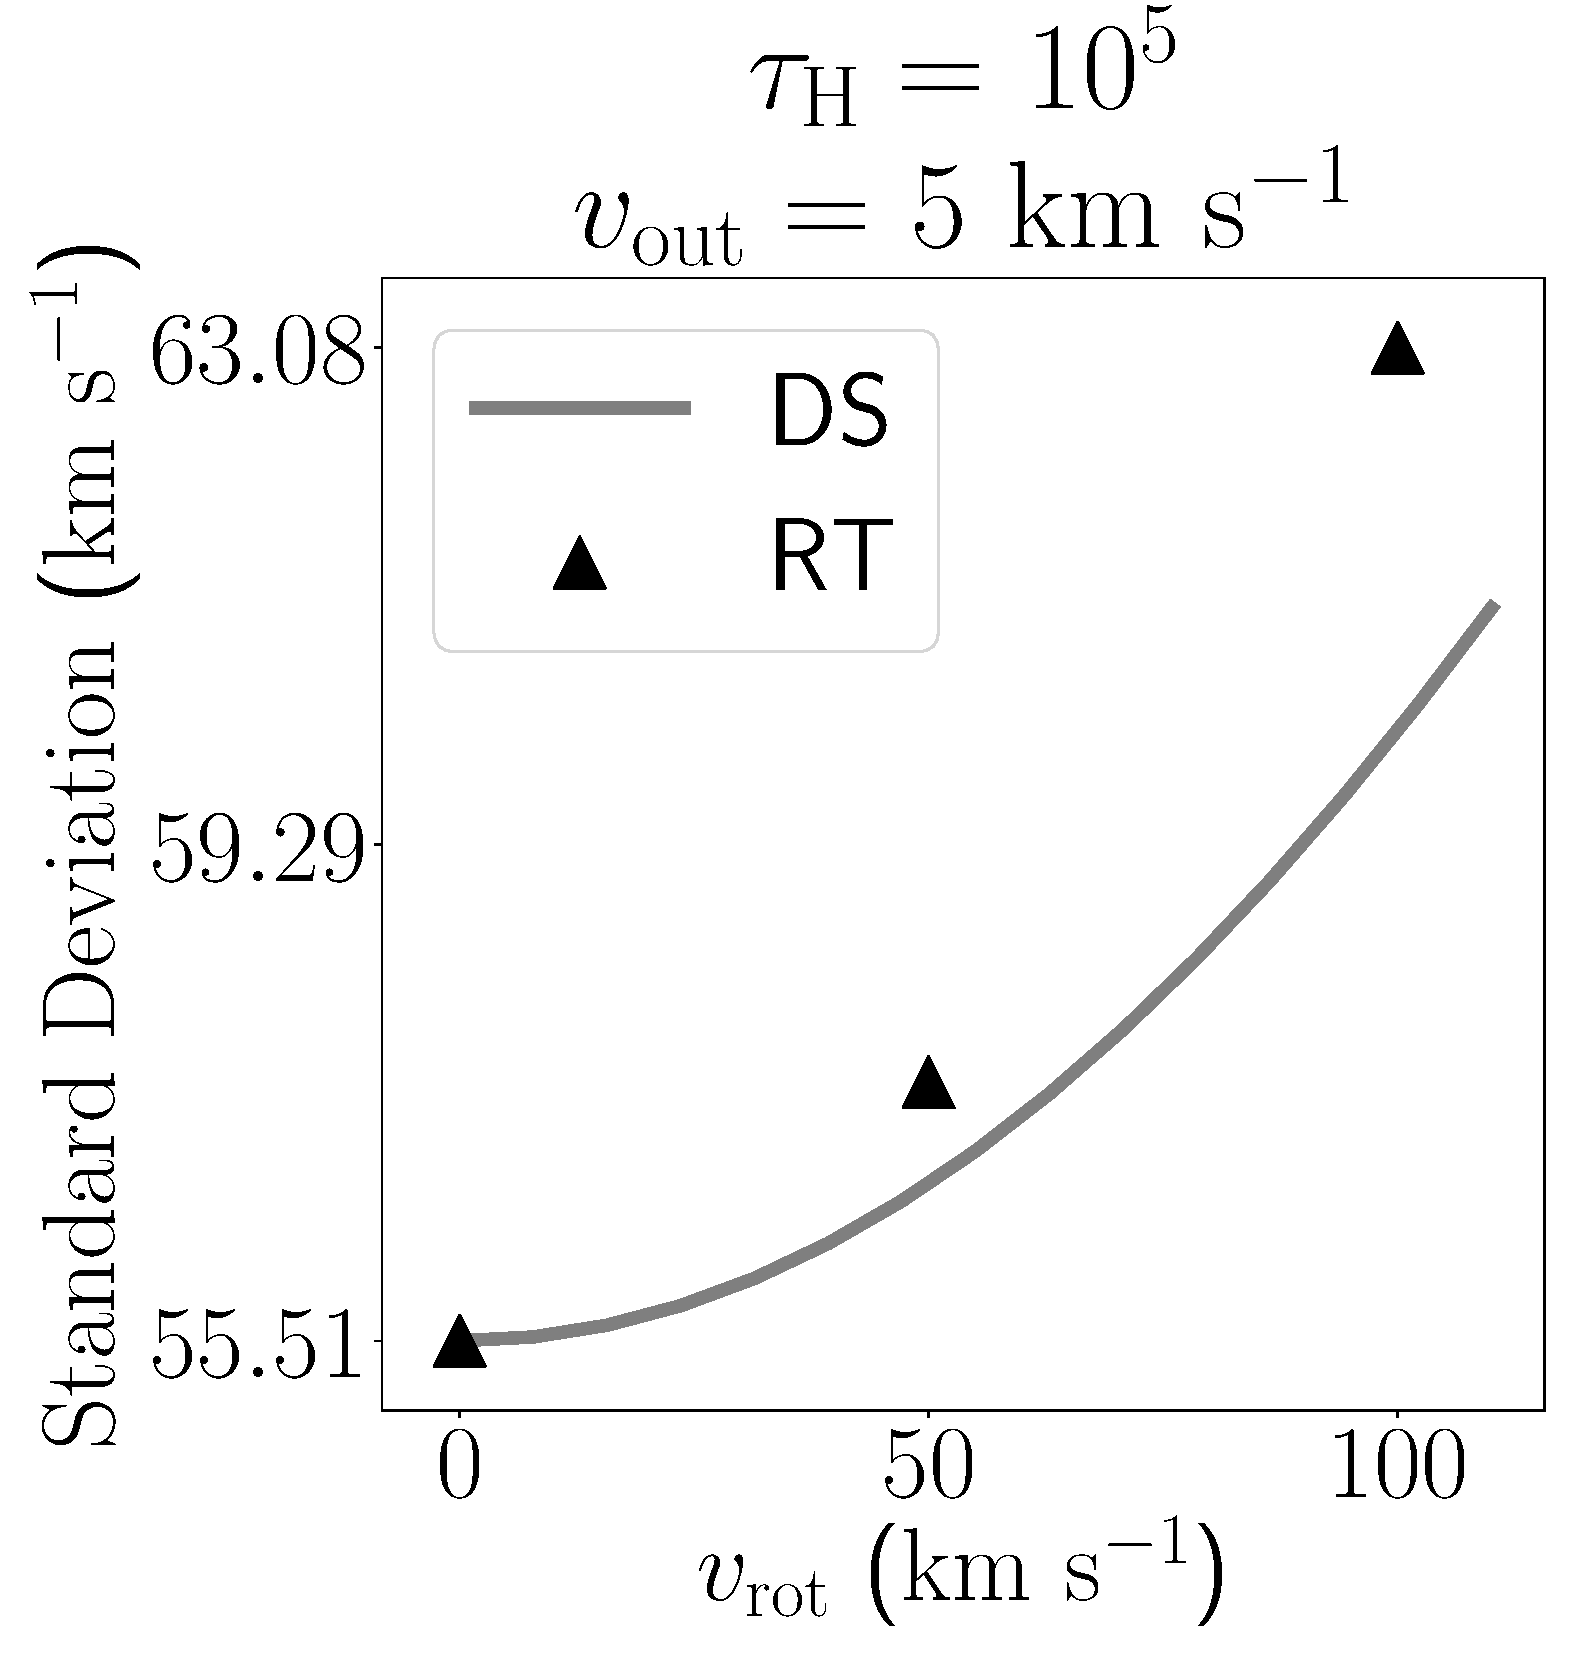
\includegraphics[height=0.27\textwidth]{./figures/results/line_characterization_std_vout5_logtau5.pdf}
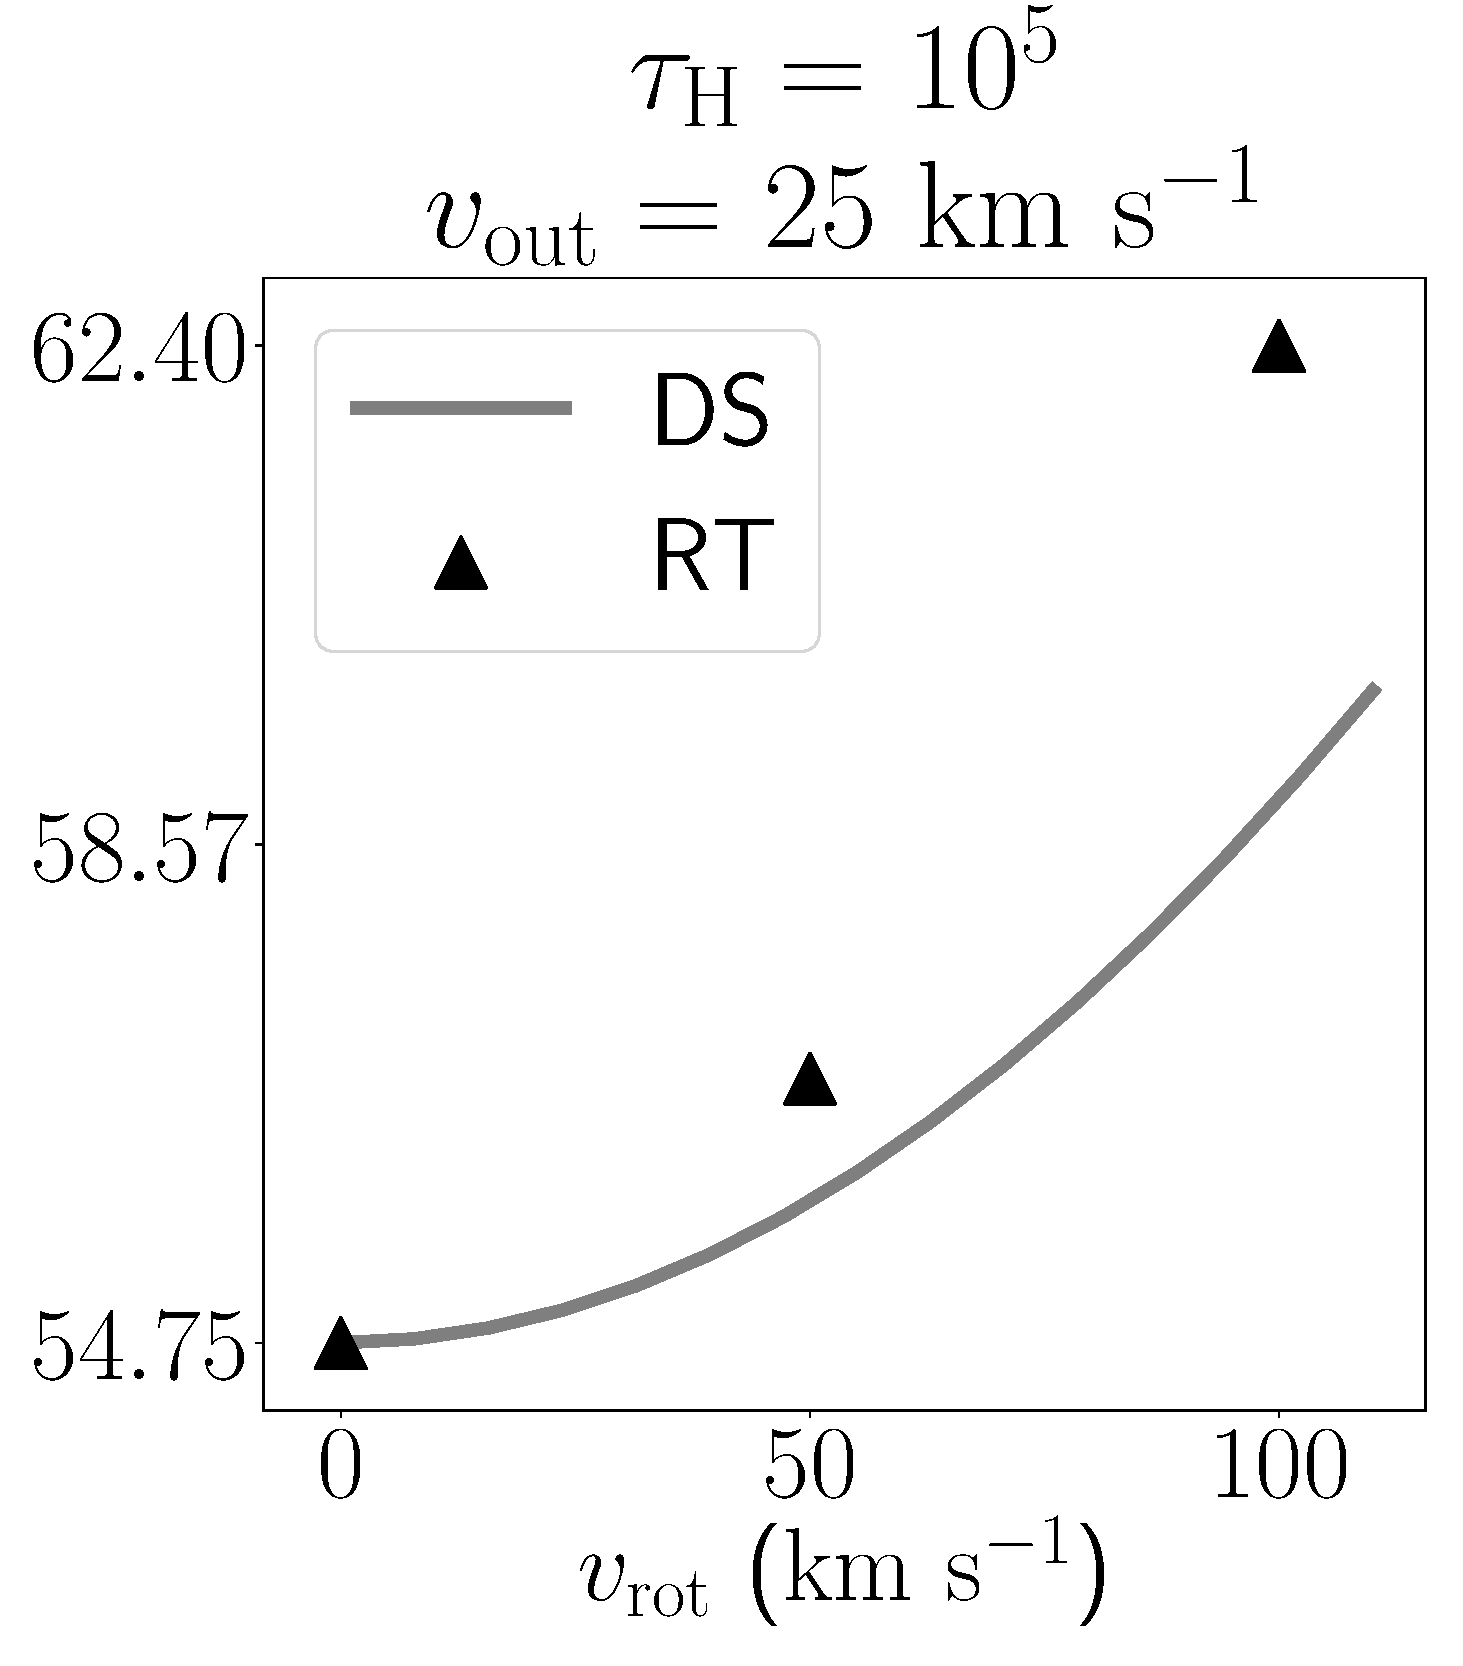
\includegraphics[height=0.27\textwidth]{./figures/results/line_characterization_std_vout25_logtau5.pdf}
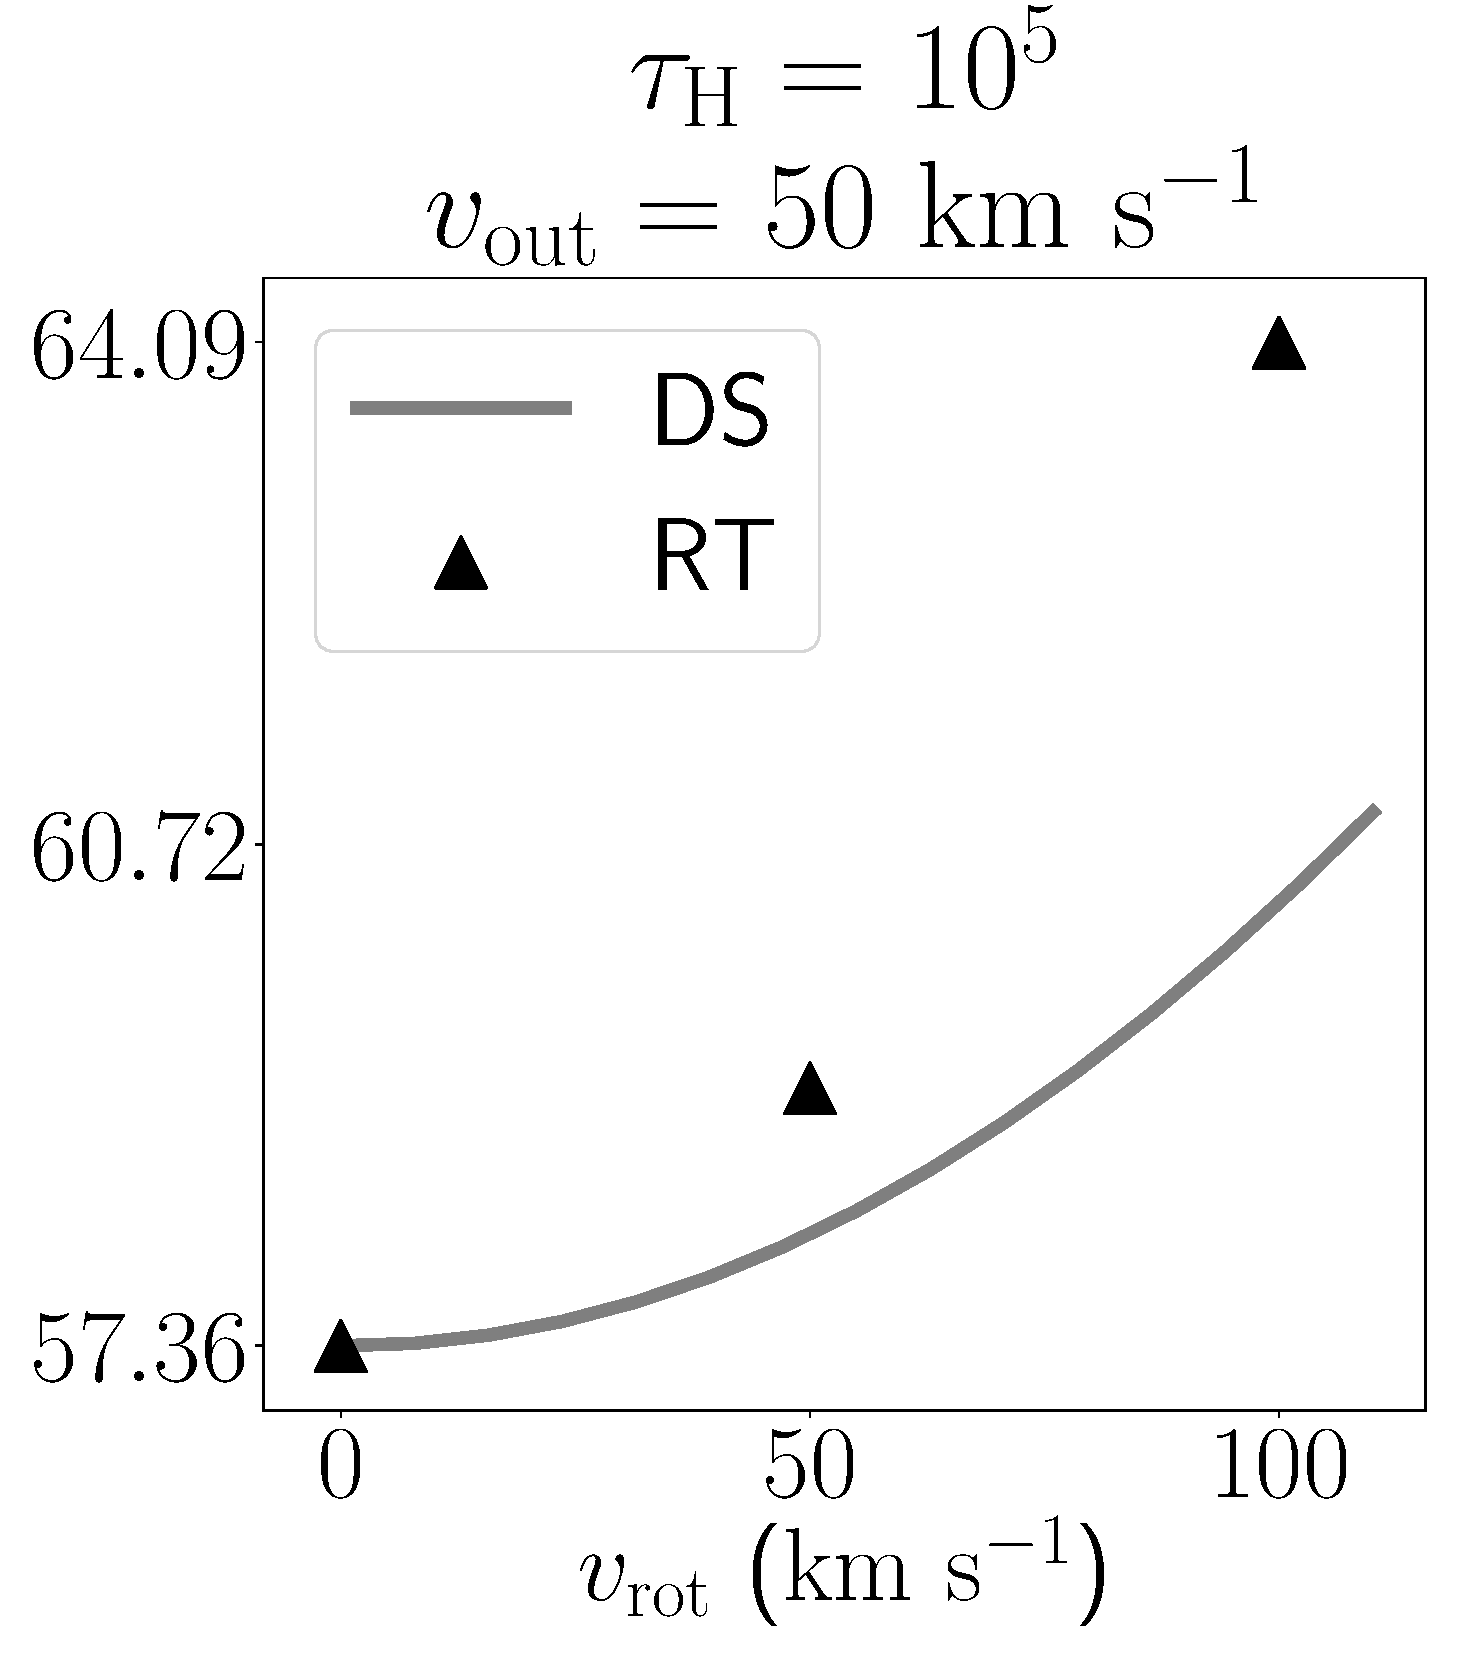
\includegraphics[height=0.27\textwidth]{./figures/results/line_characterization_std_vout50_logtau5.pdf}
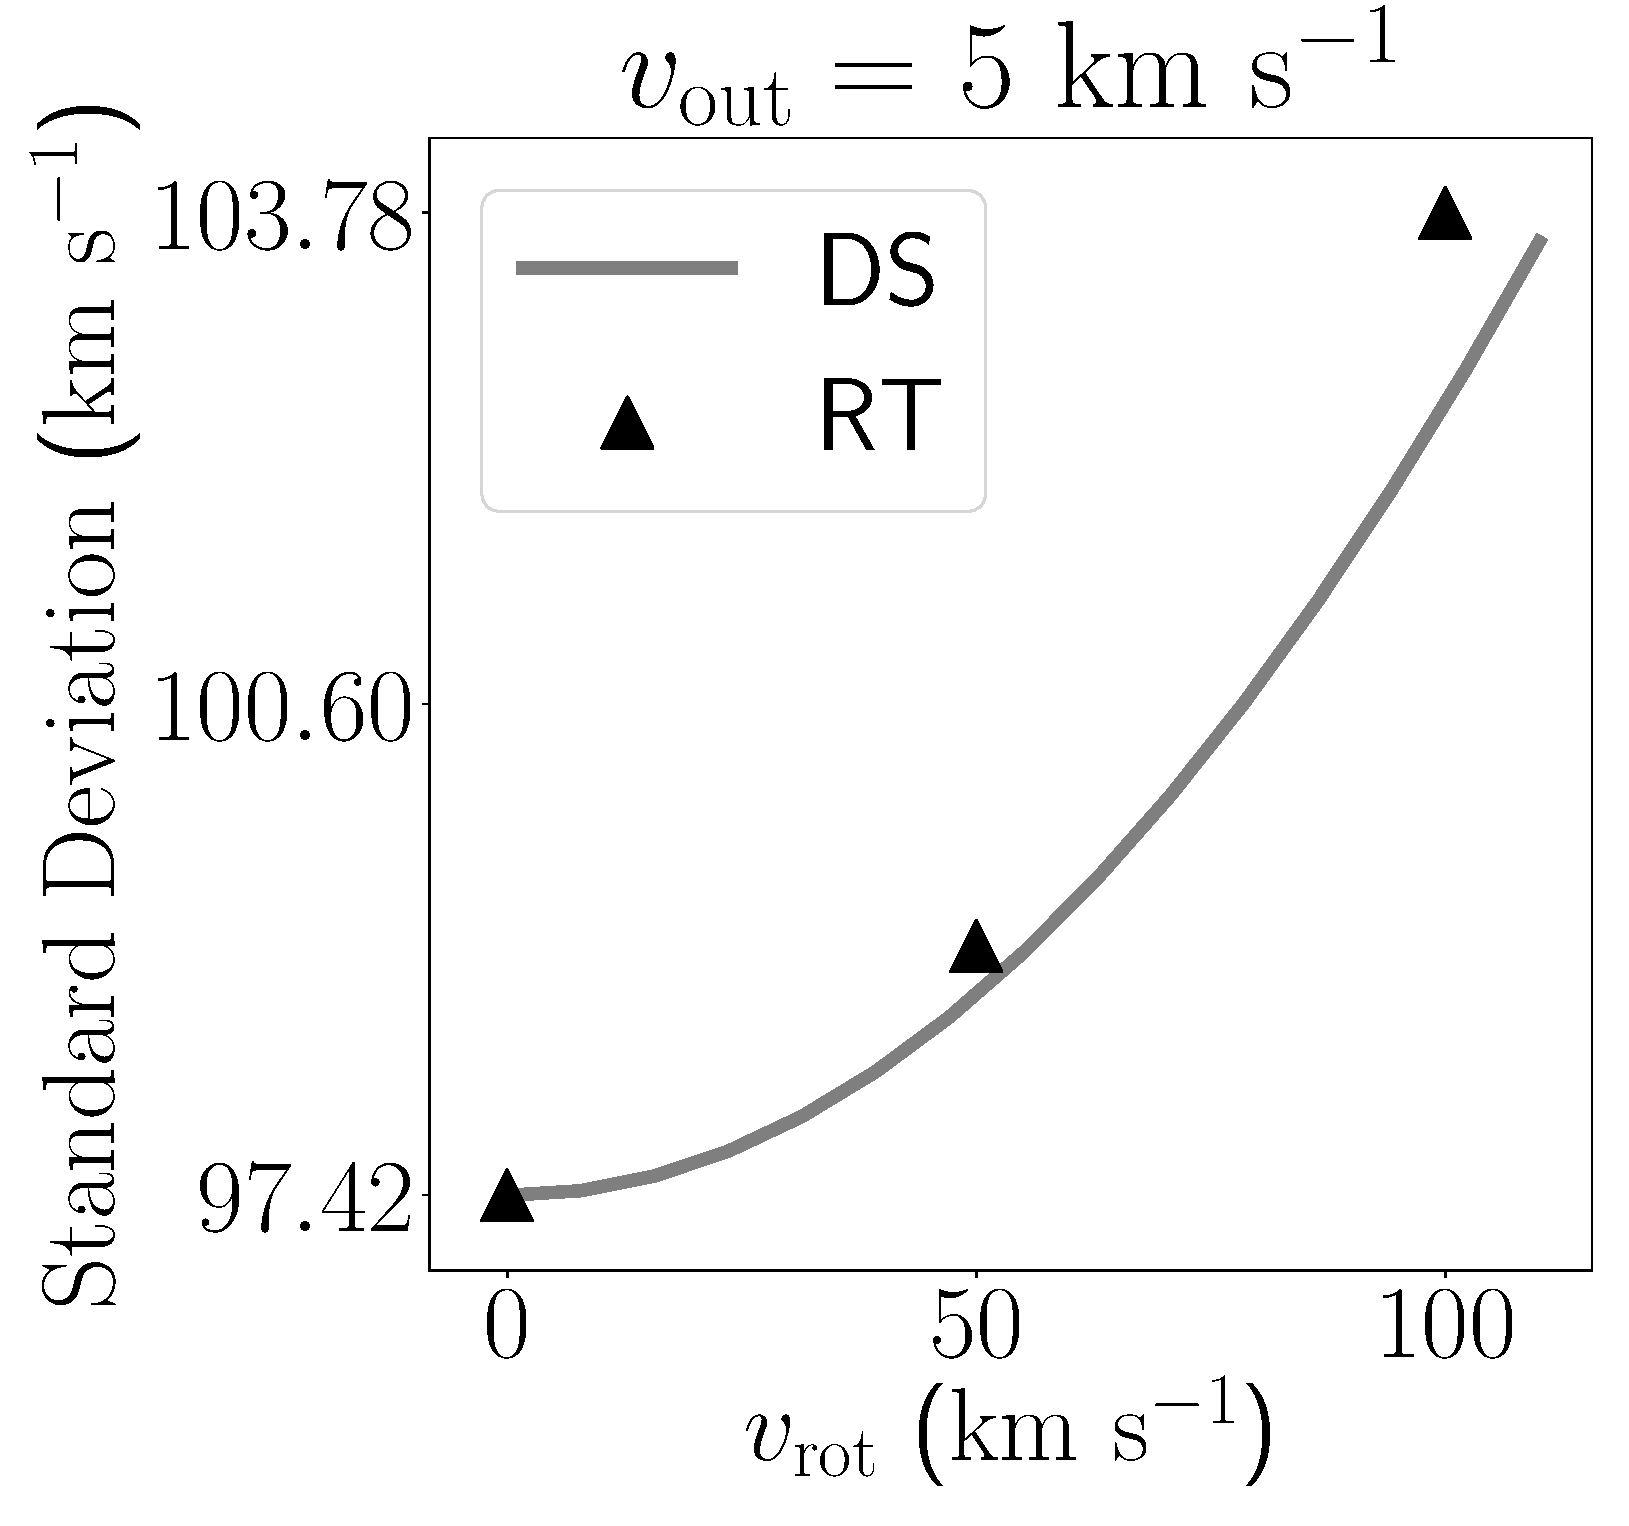
\includegraphics[height=0.27\textwidth]{./figures/results/line_characterization_std_vout5_logtau6.pdf}
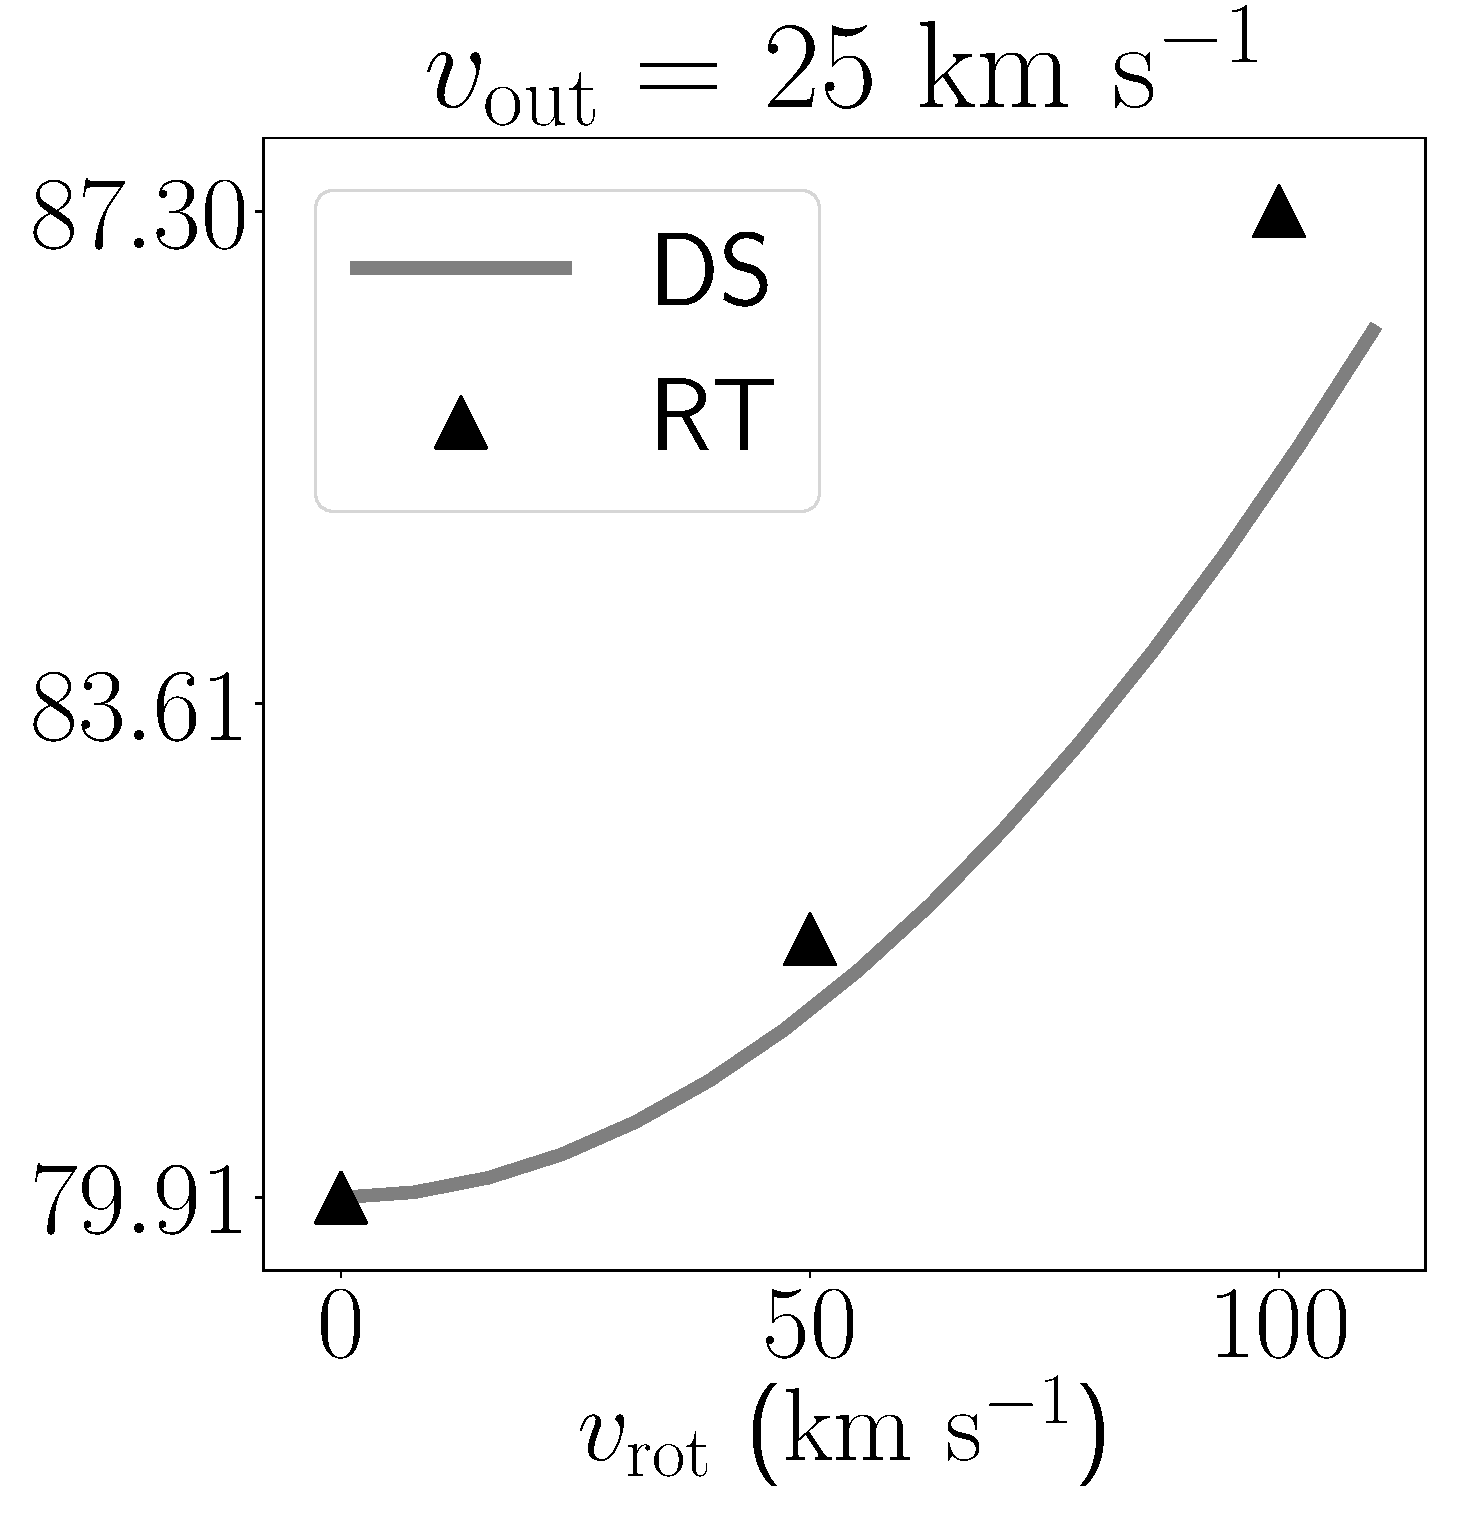
\includegraphics[height=0.27\textwidth]{./figures/results/line_characterization_std_vout25_logtau6.pdf}
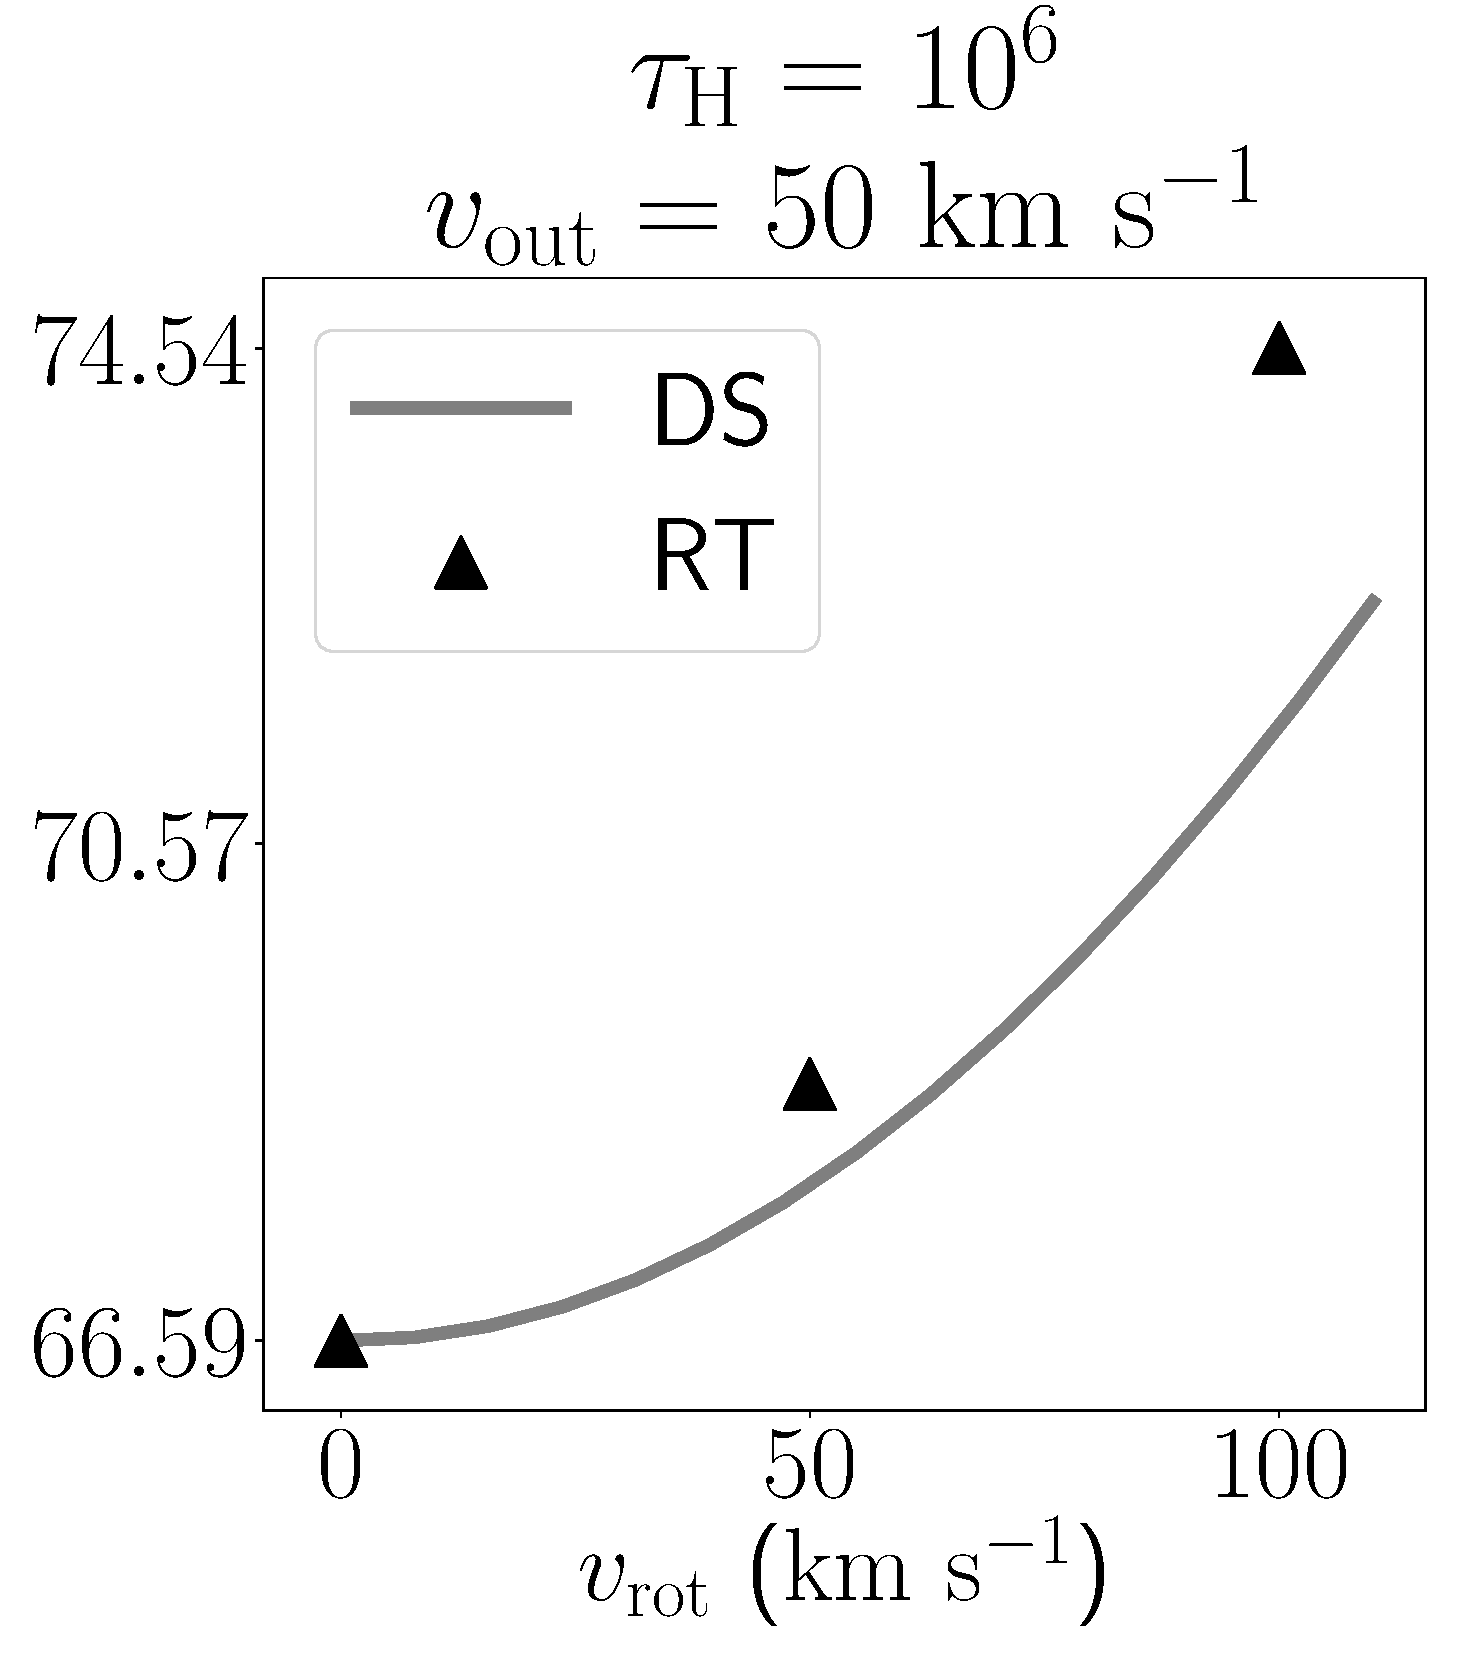
\includegraphics[height=0.27\textwidth]{./figures/results/line_characterization_std_vout50_logtau6.pdf}
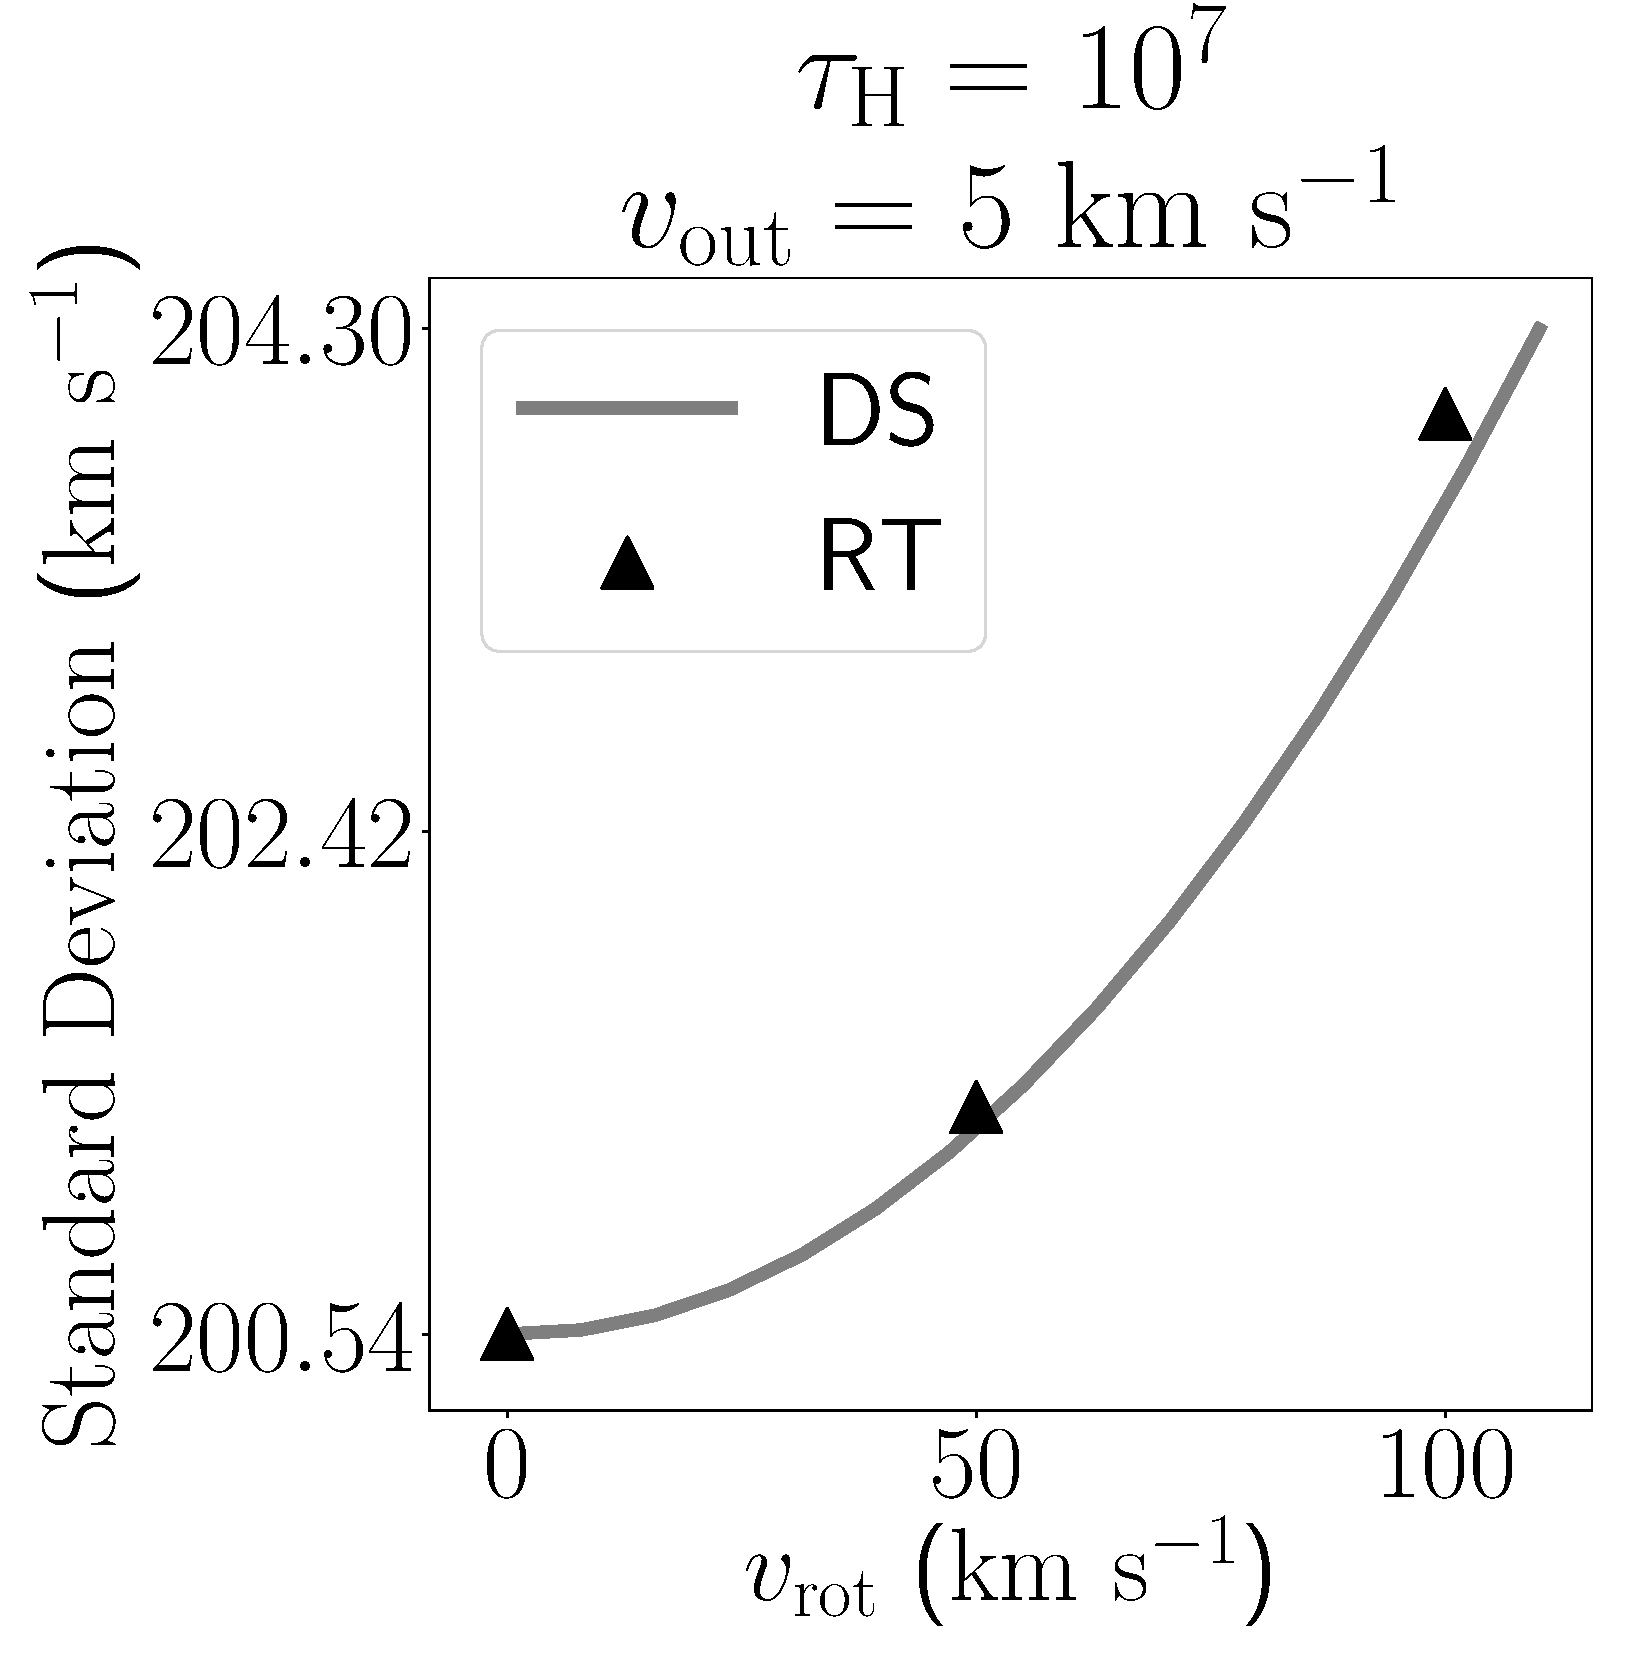
\includegraphics[height=0.27\textwidth]{./figures/results/line_characterization_std_vout5_logtau7.pdf}
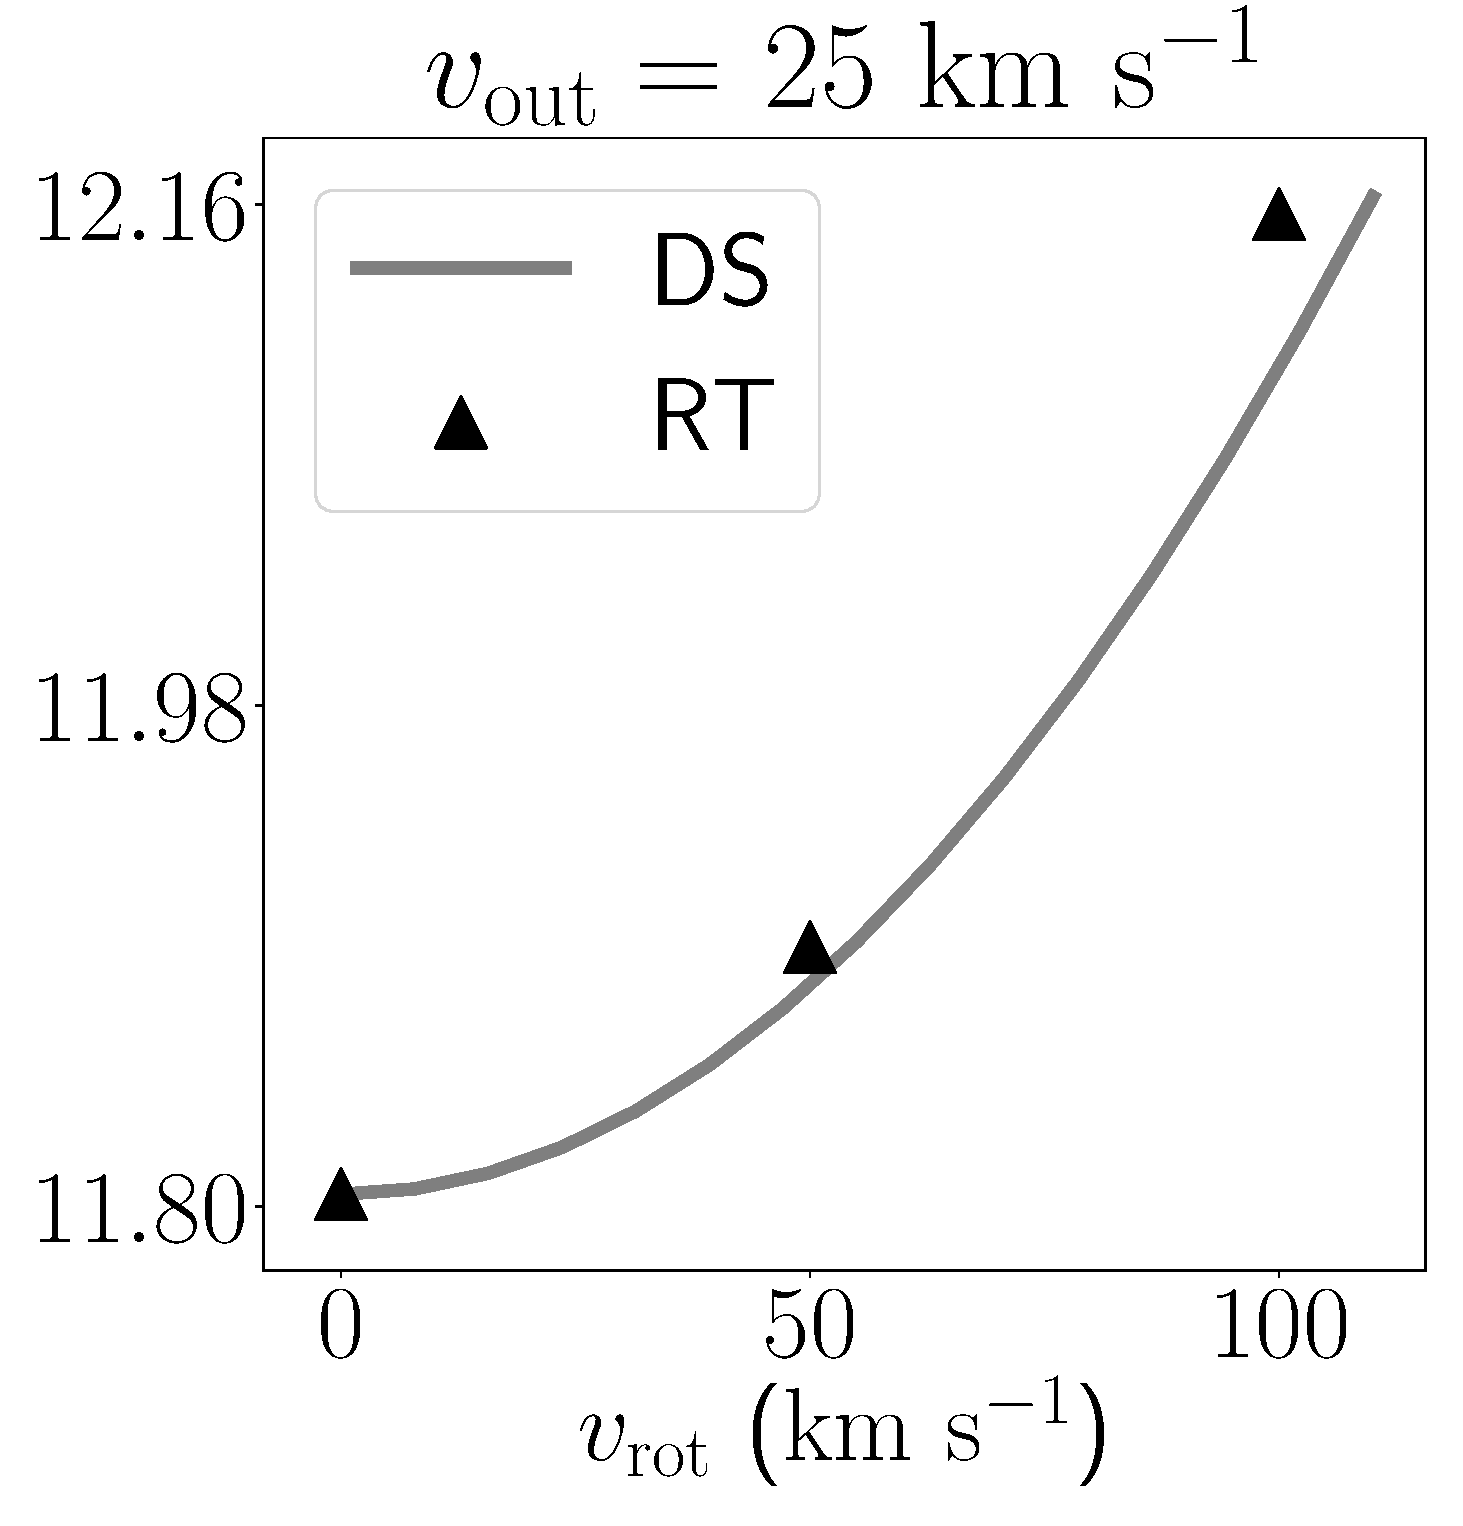
\includegraphics[height=0.27\textwidth]{./figures/results/line_characterization_std_vout25_logtau7.pdf}
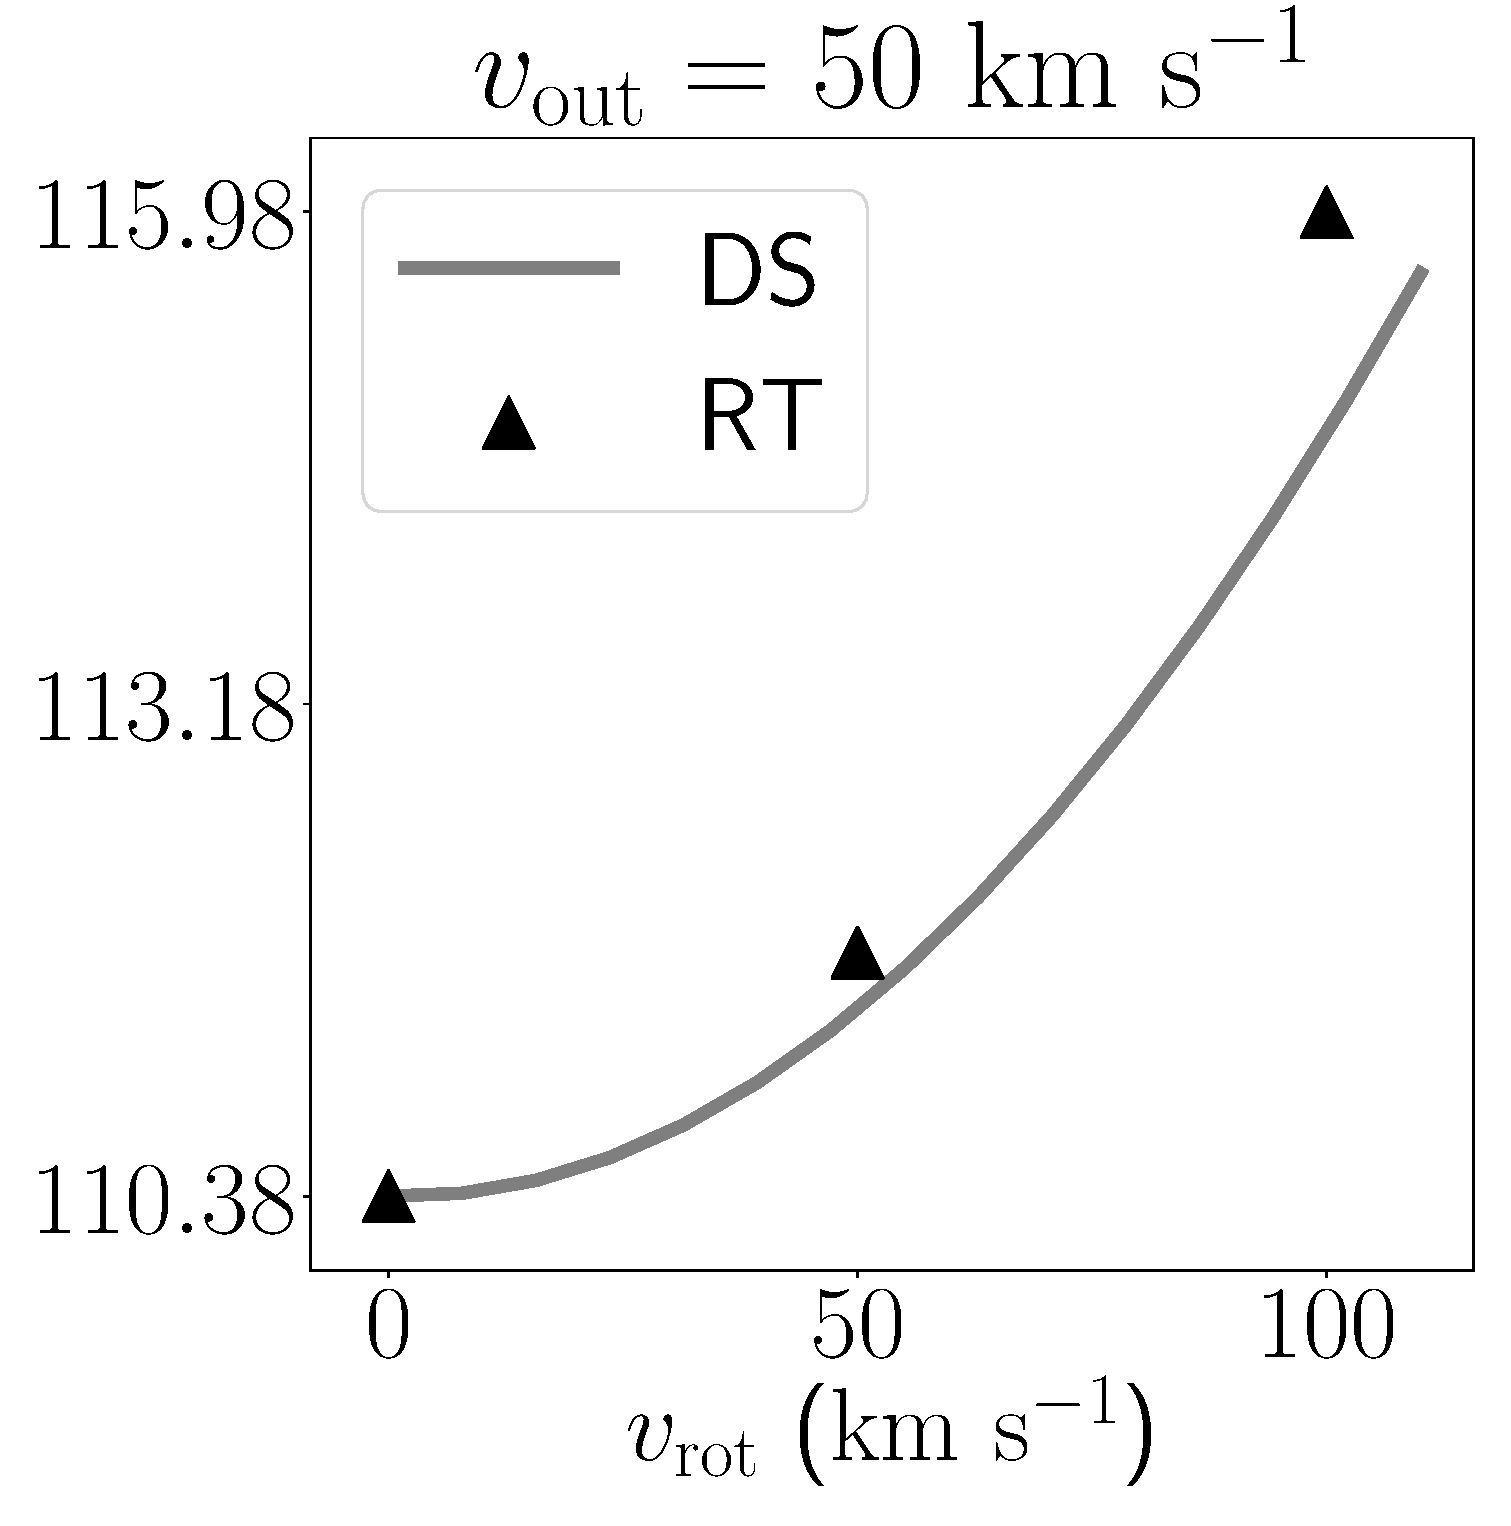
\includegraphics[height=0.27\textwidth]{./figures/results/line_characterization_std_vout50_logtau7.pdf}
\end{center}
\caption{\textbf{Standard Deviation trends.} Results for all the
  Radiative Transfer simulations (in triangles) compares against the
  Doppler Shift model (lines).
  All panels correspond to a viewing angle of $\theta = 90^{\circ}$
  (perpendicular to the rotation axis). 
  The optical depth increases from top to bottom and the outflow
  velocity from left to right.
  \label{fig:standard_deviation}}
\end{figure*}

\begin{figure*}
\begin{center}
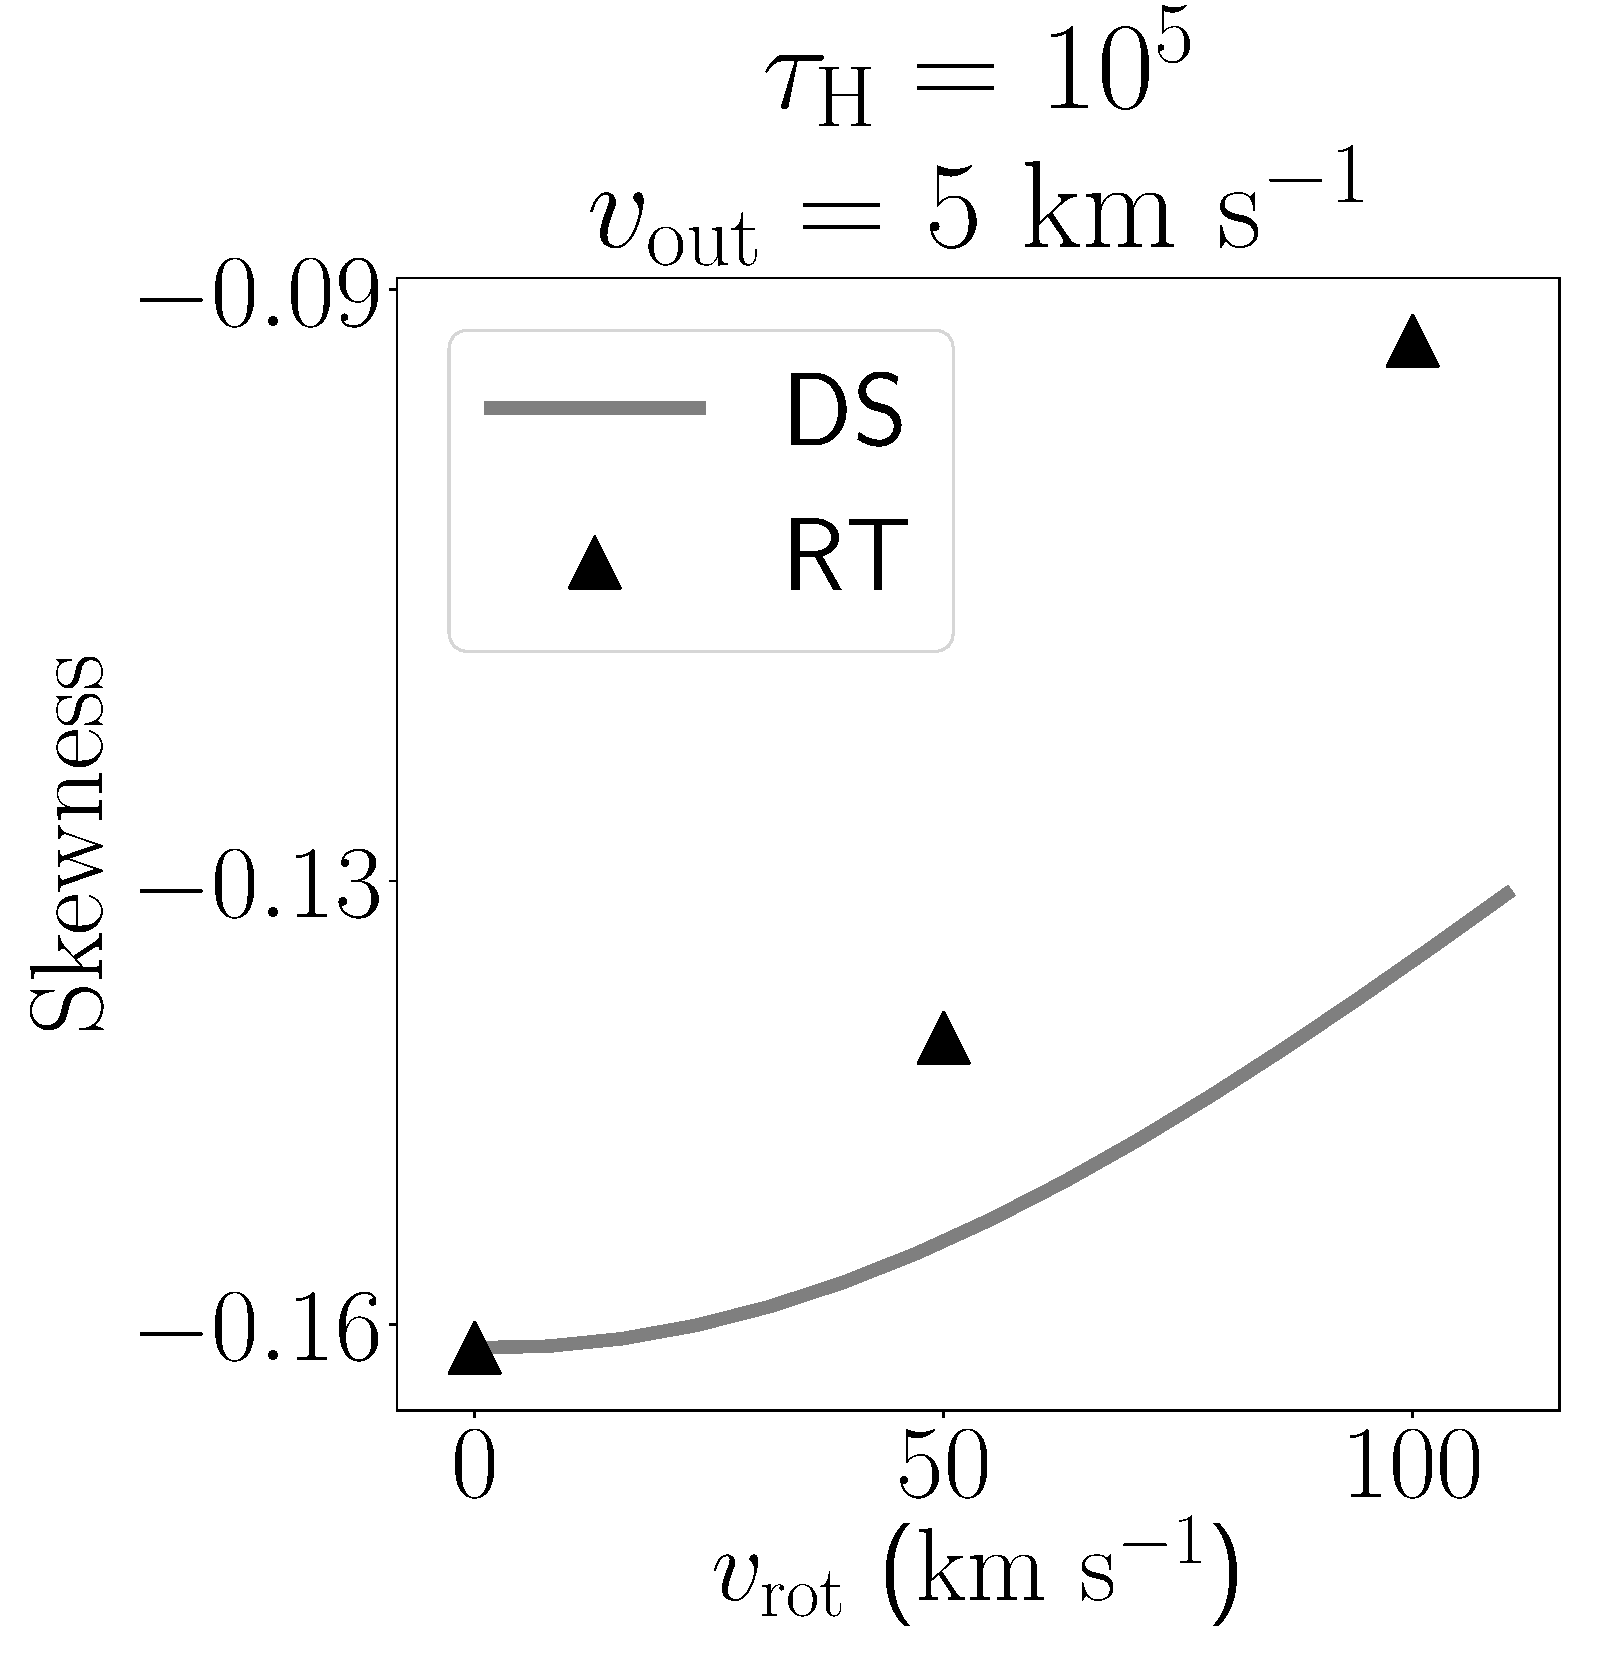
\includegraphics[height=0.27\textwidth]{./figures/results/line_characterization_skw_vout5_logtau5}
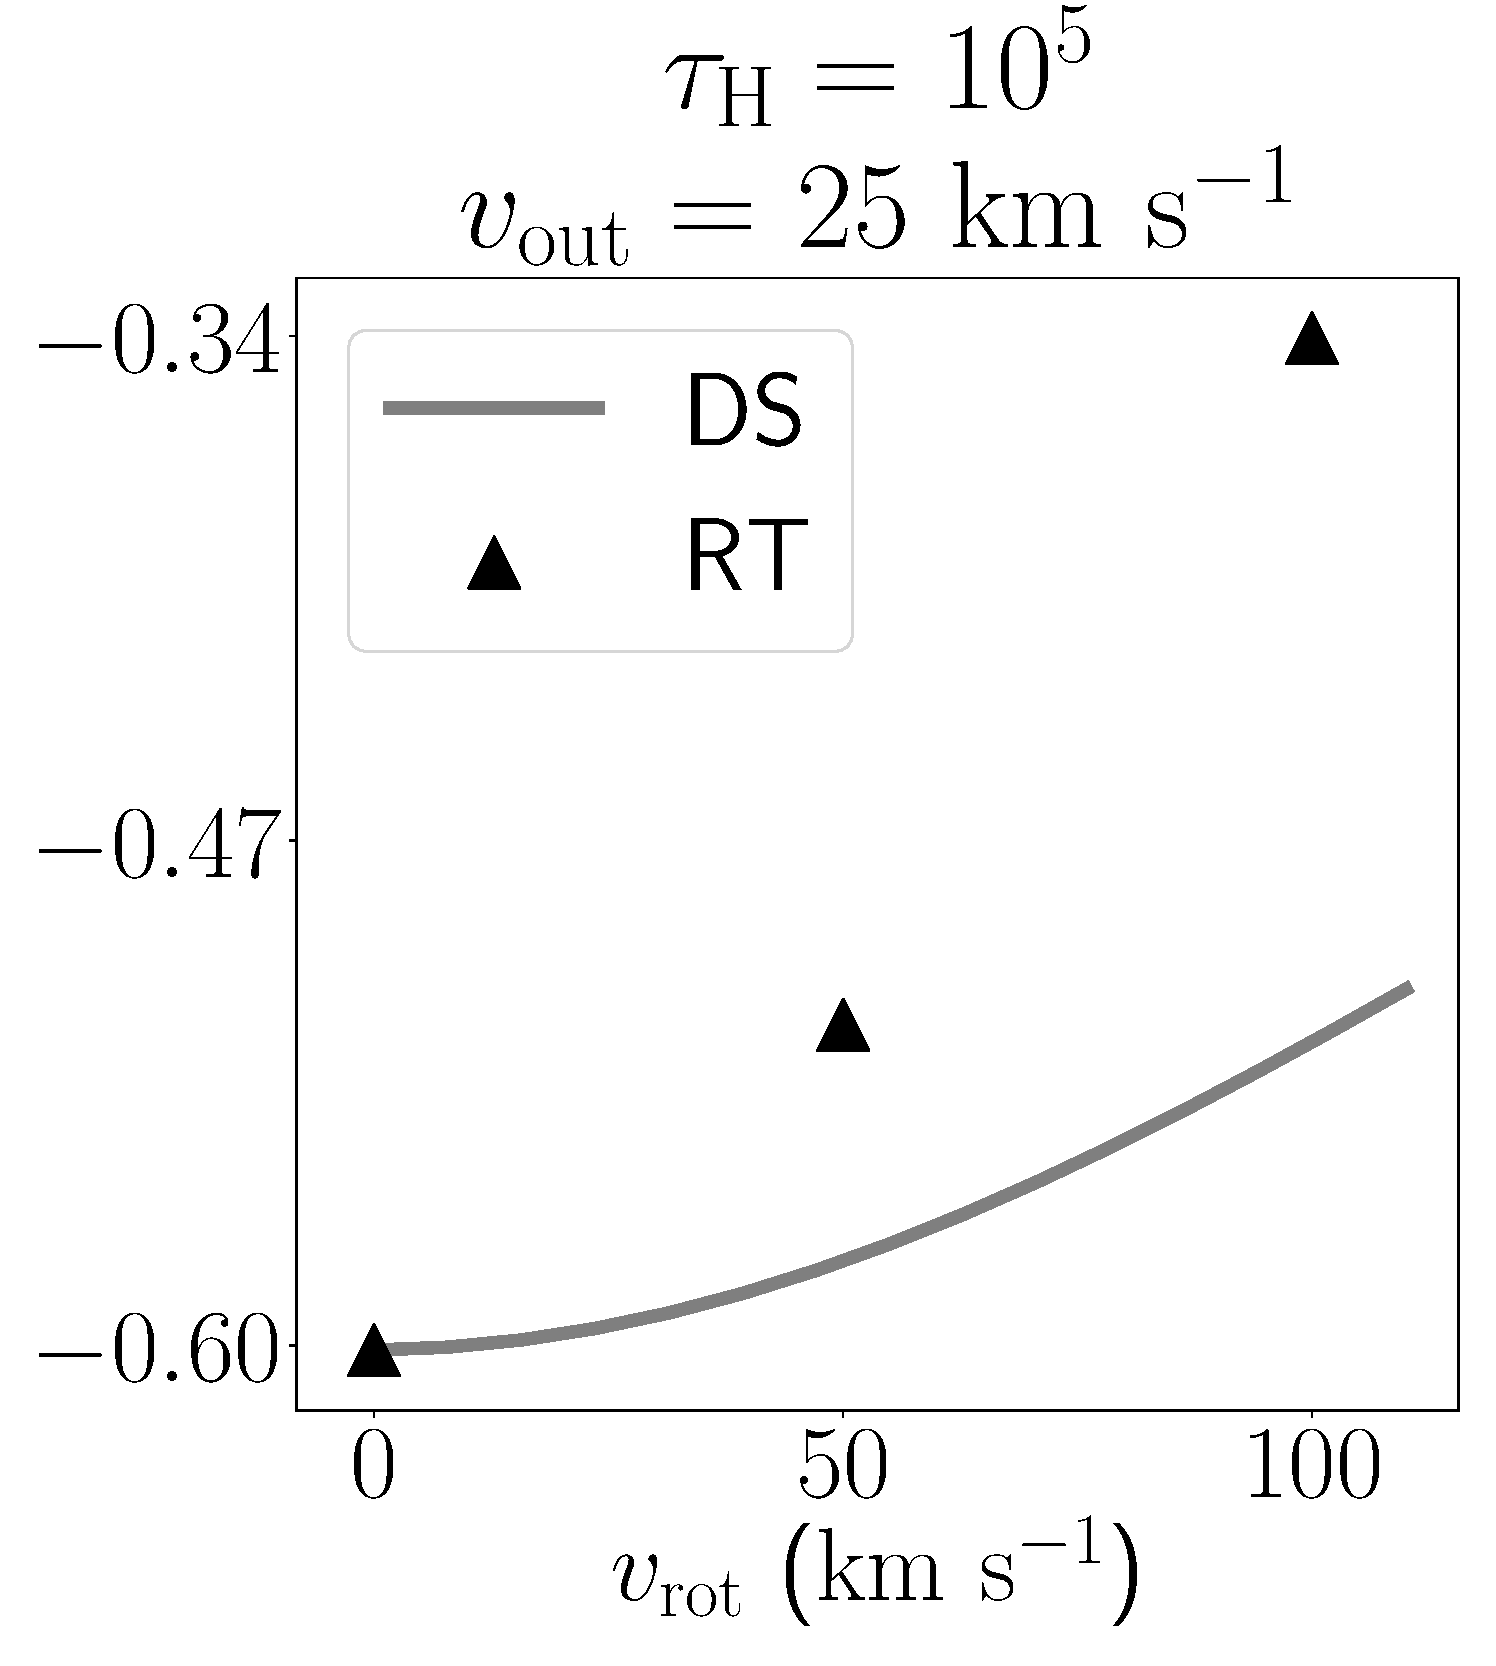
\includegraphics[height=0.27\textwidth]{./figures/results/line_characterization_skw_vout25_logtau5}
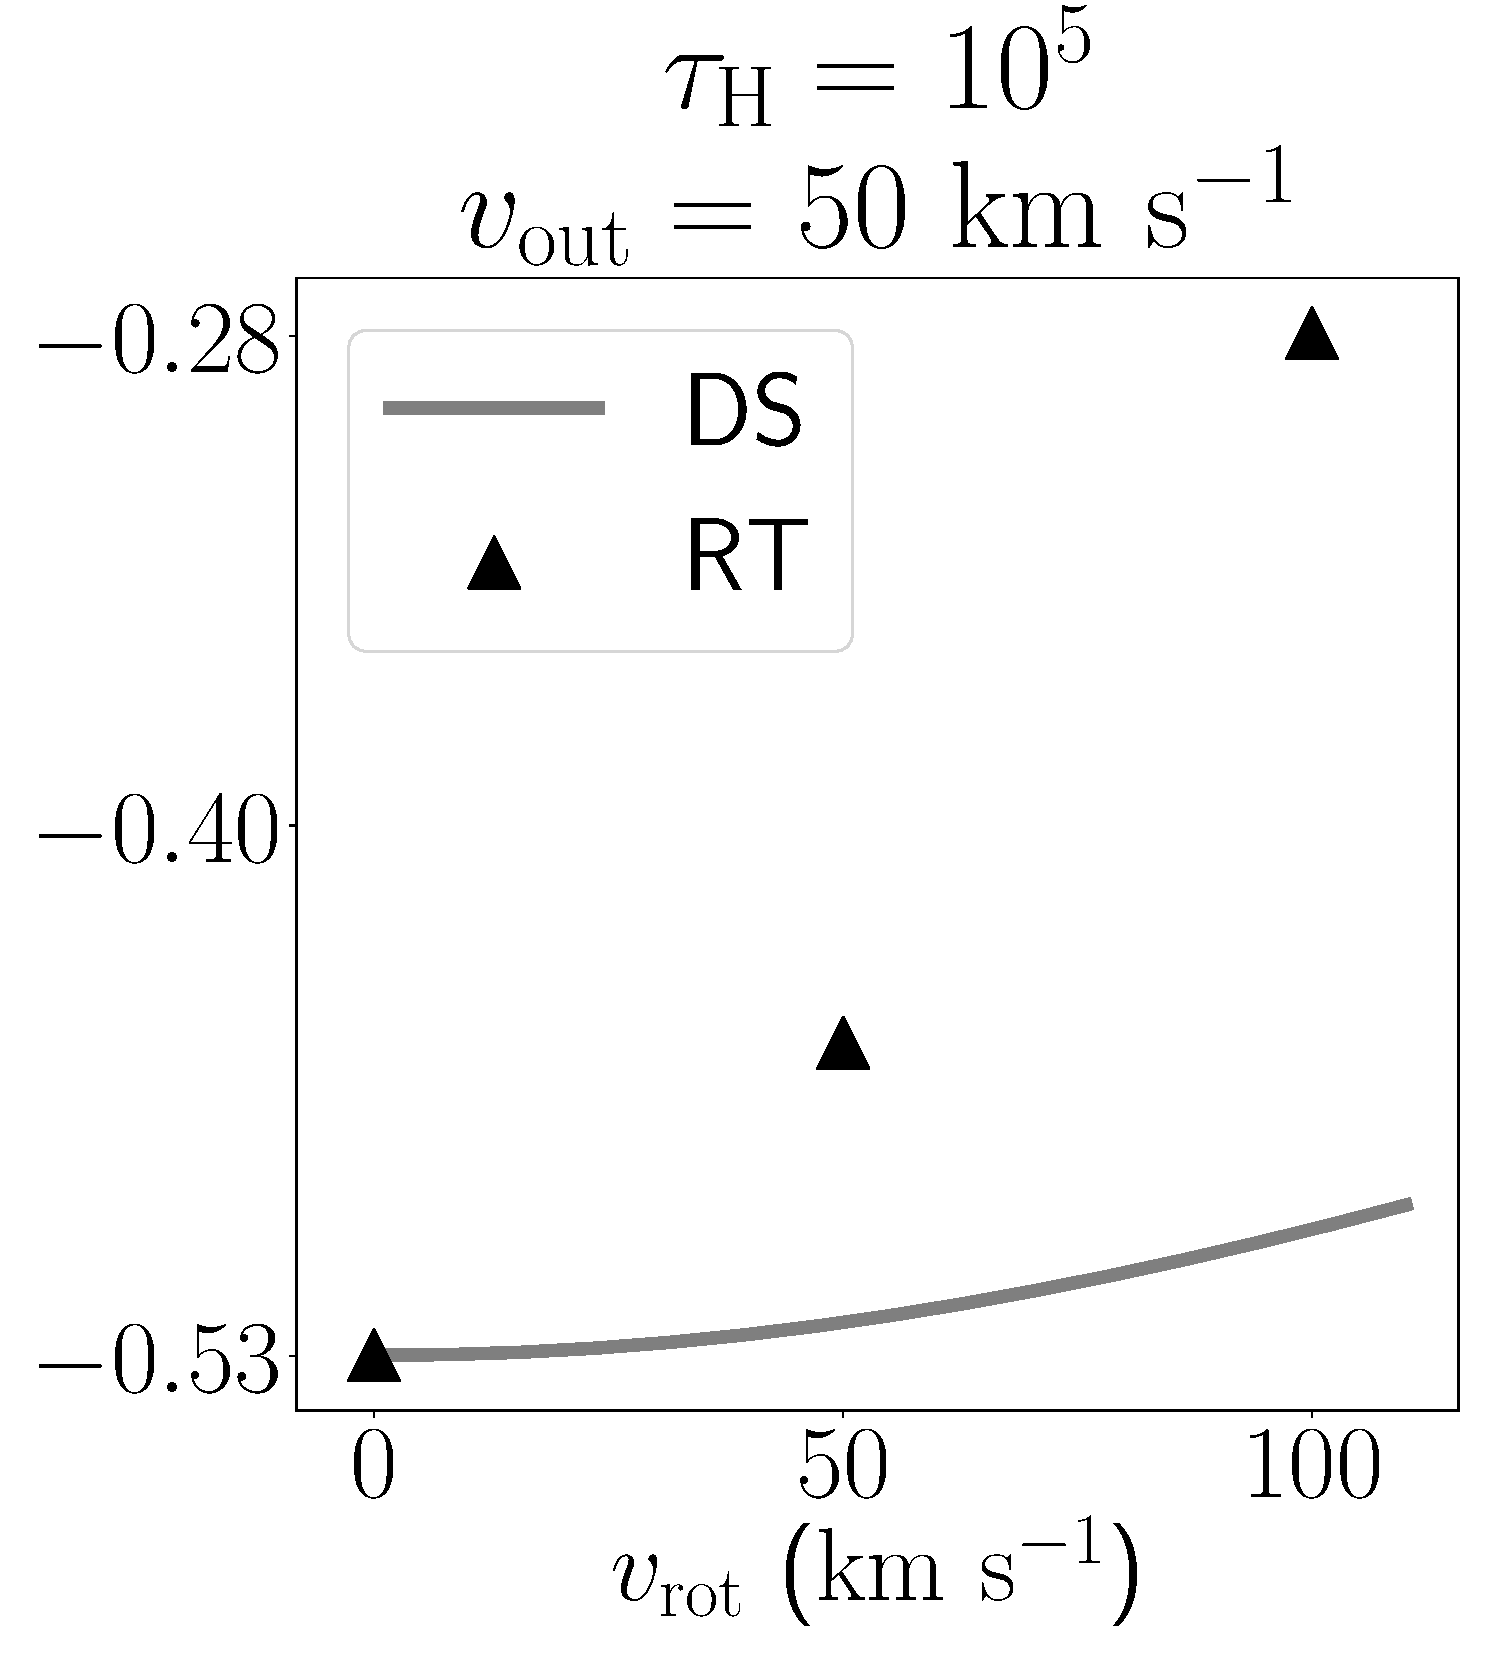
\includegraphics[height=0.27\textwidth]{./figures/results/line_characterization_skw_vout50_logtau5}
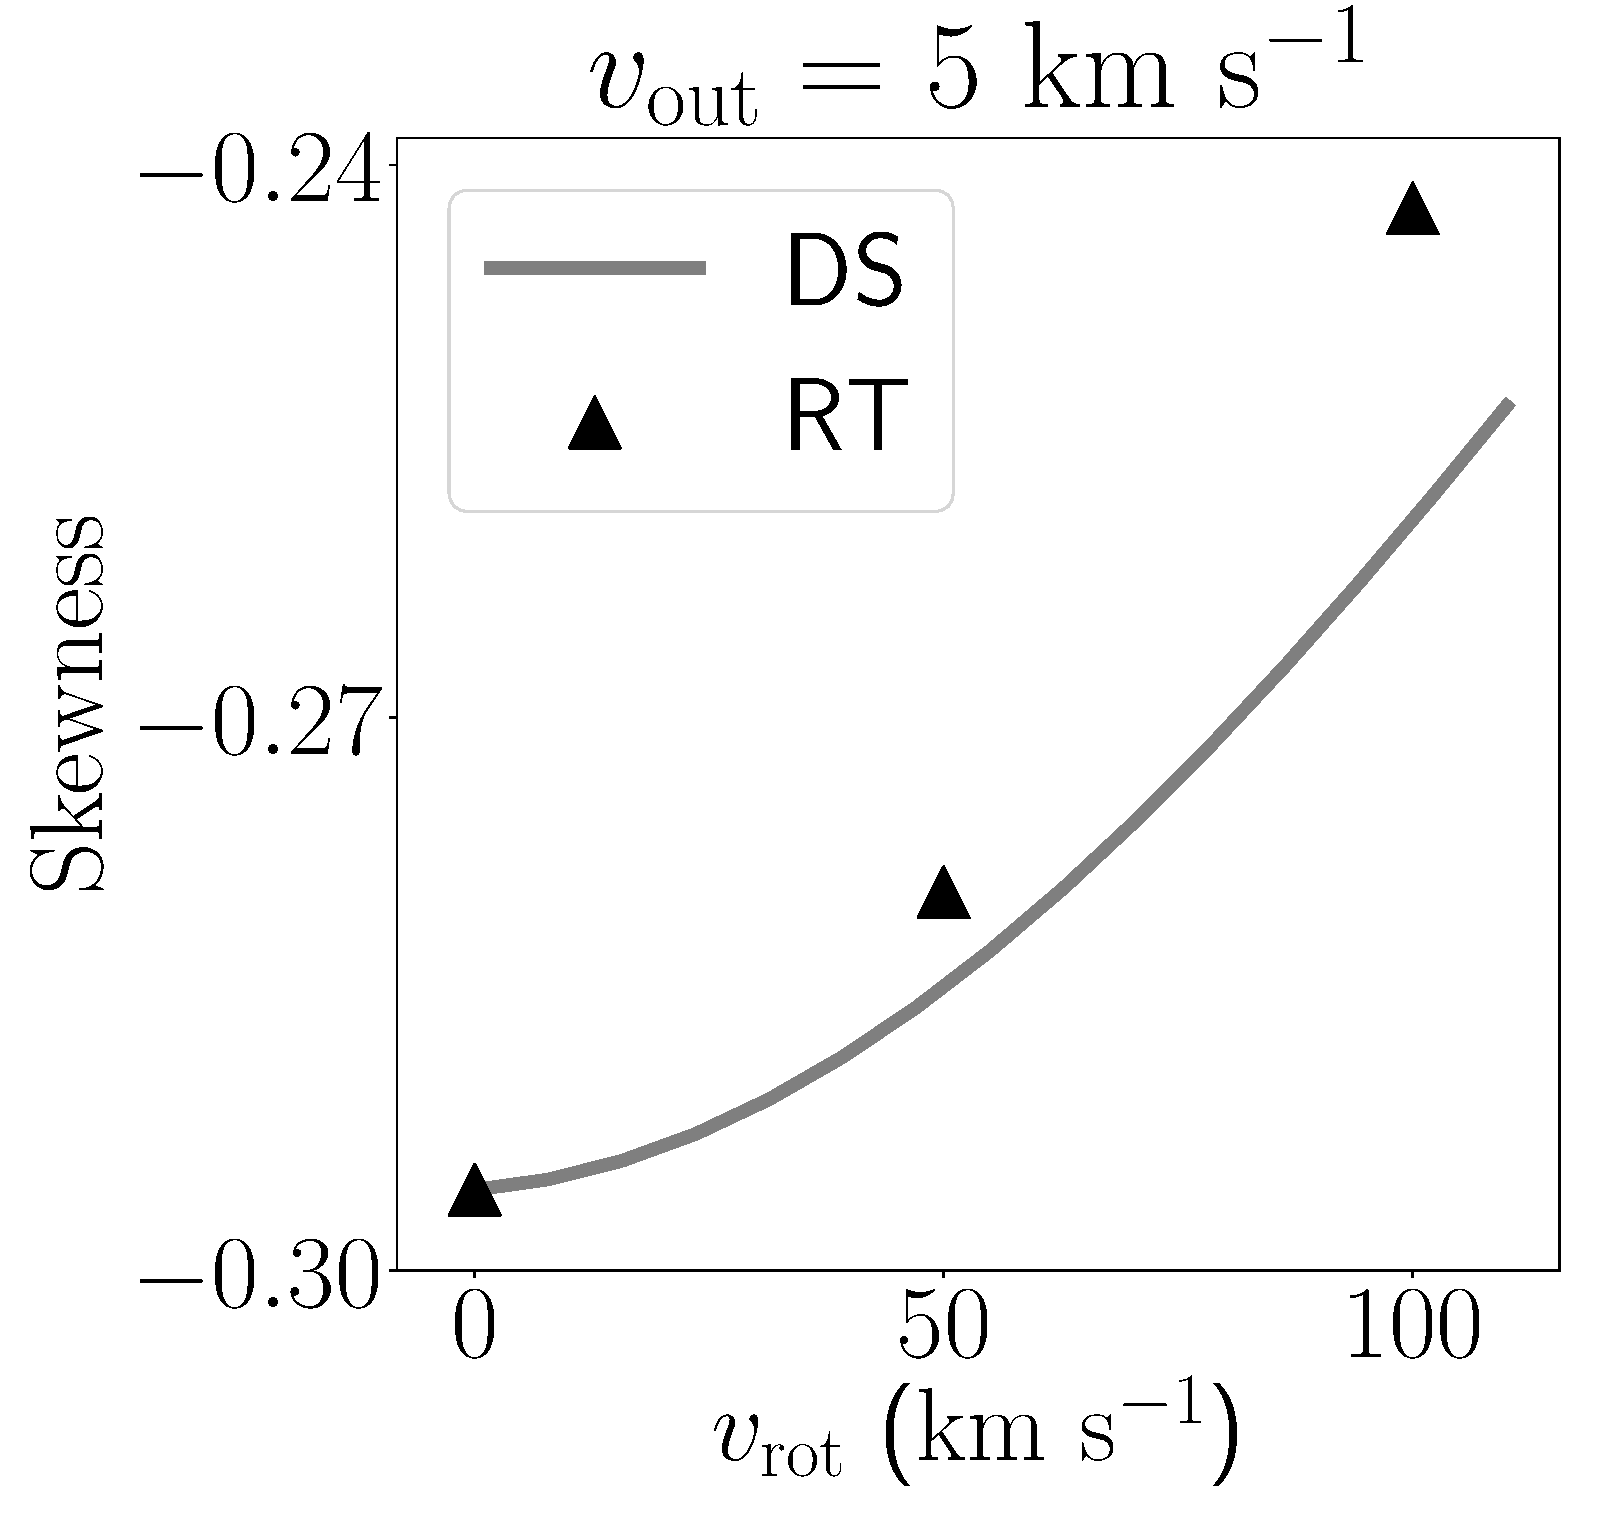
\includegraphics[height=0.27\textwidth]{./figures/results/line_characterization_skw_vout5_logtau6}
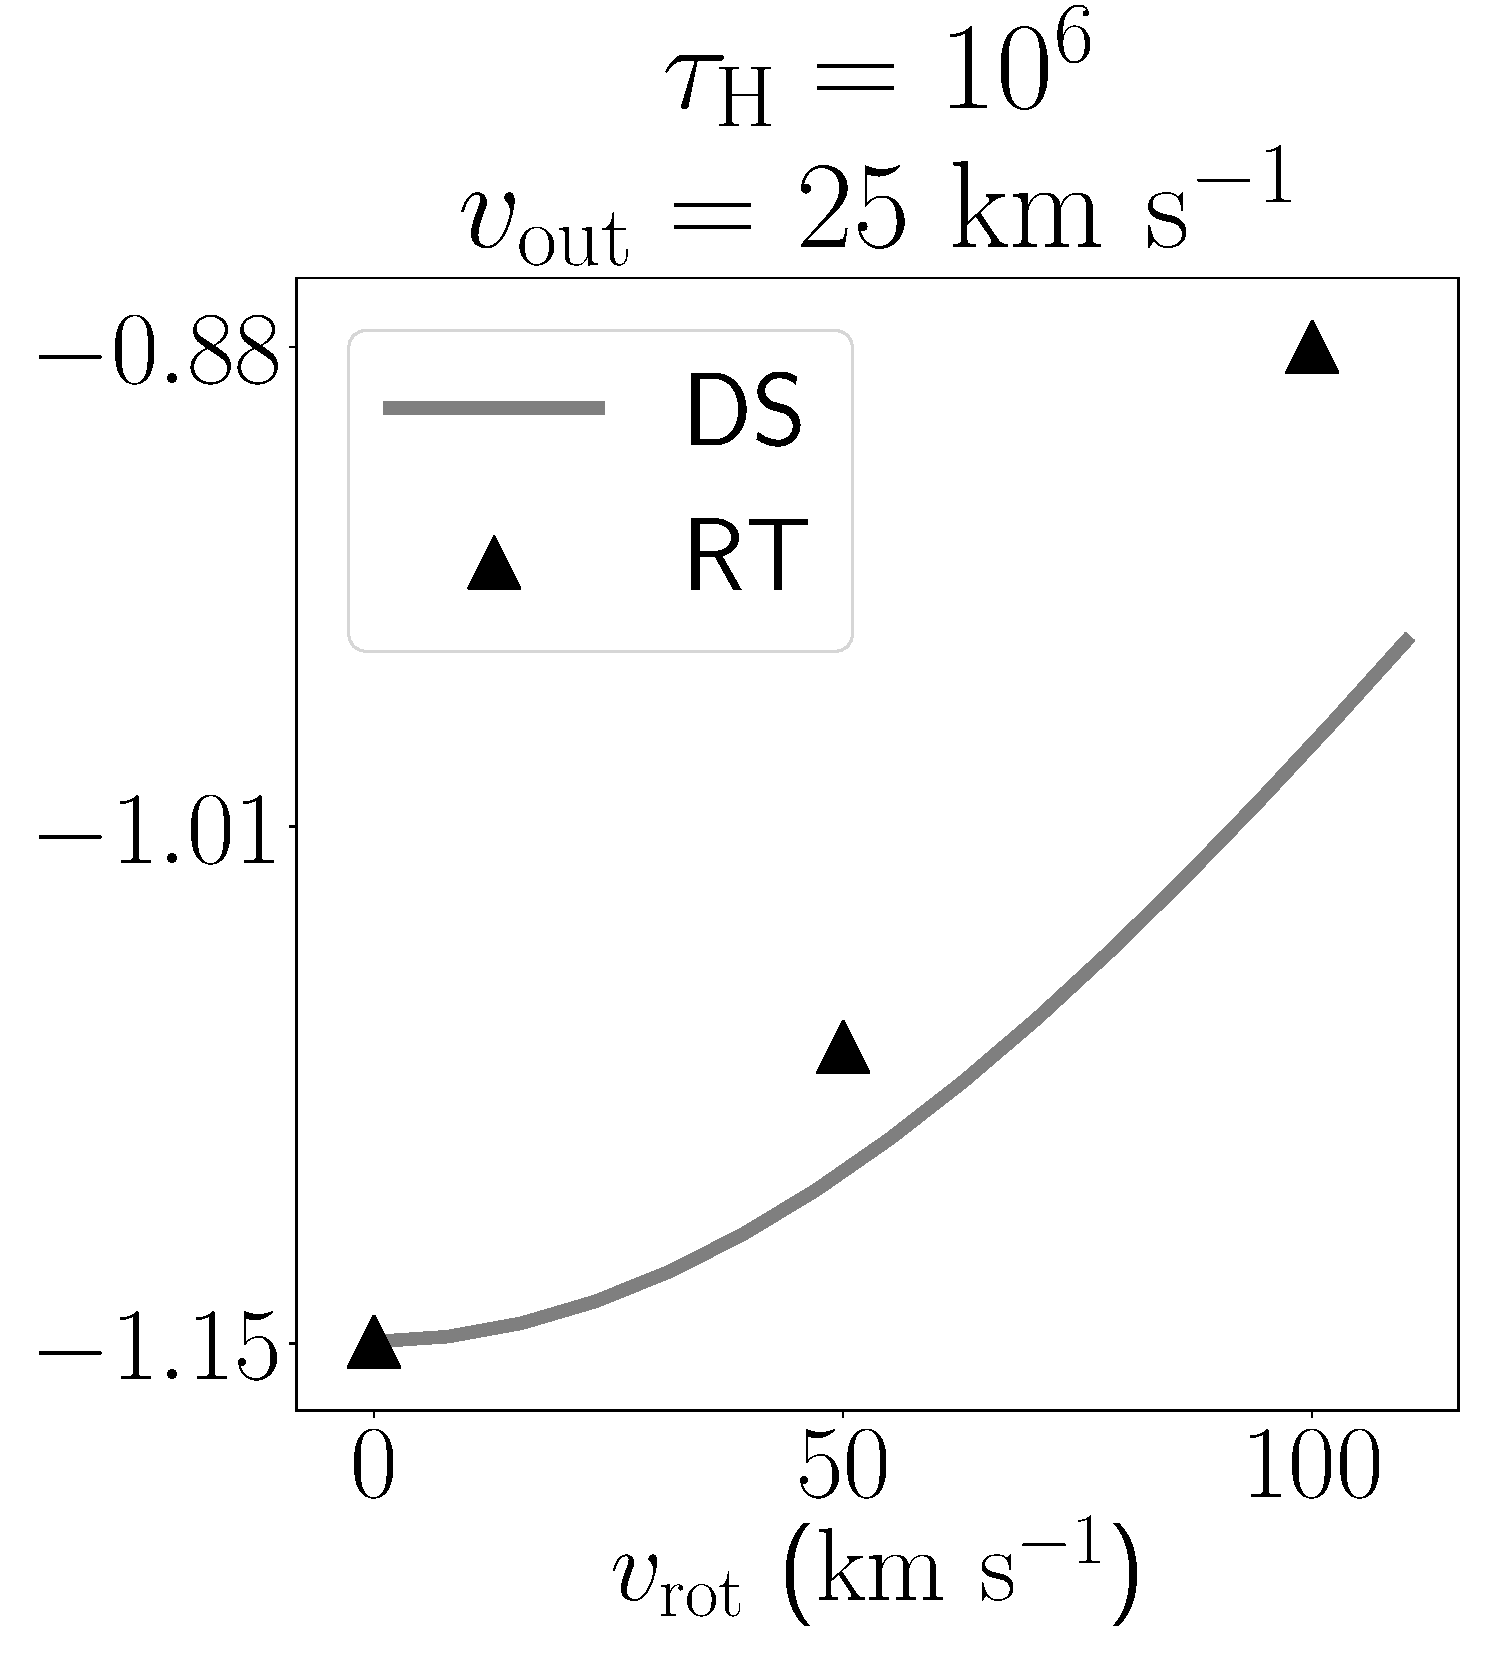
\includegraphics[height=0.27\textwidth]{./figures/results/line_characterization_skw_vout25_logtau6}
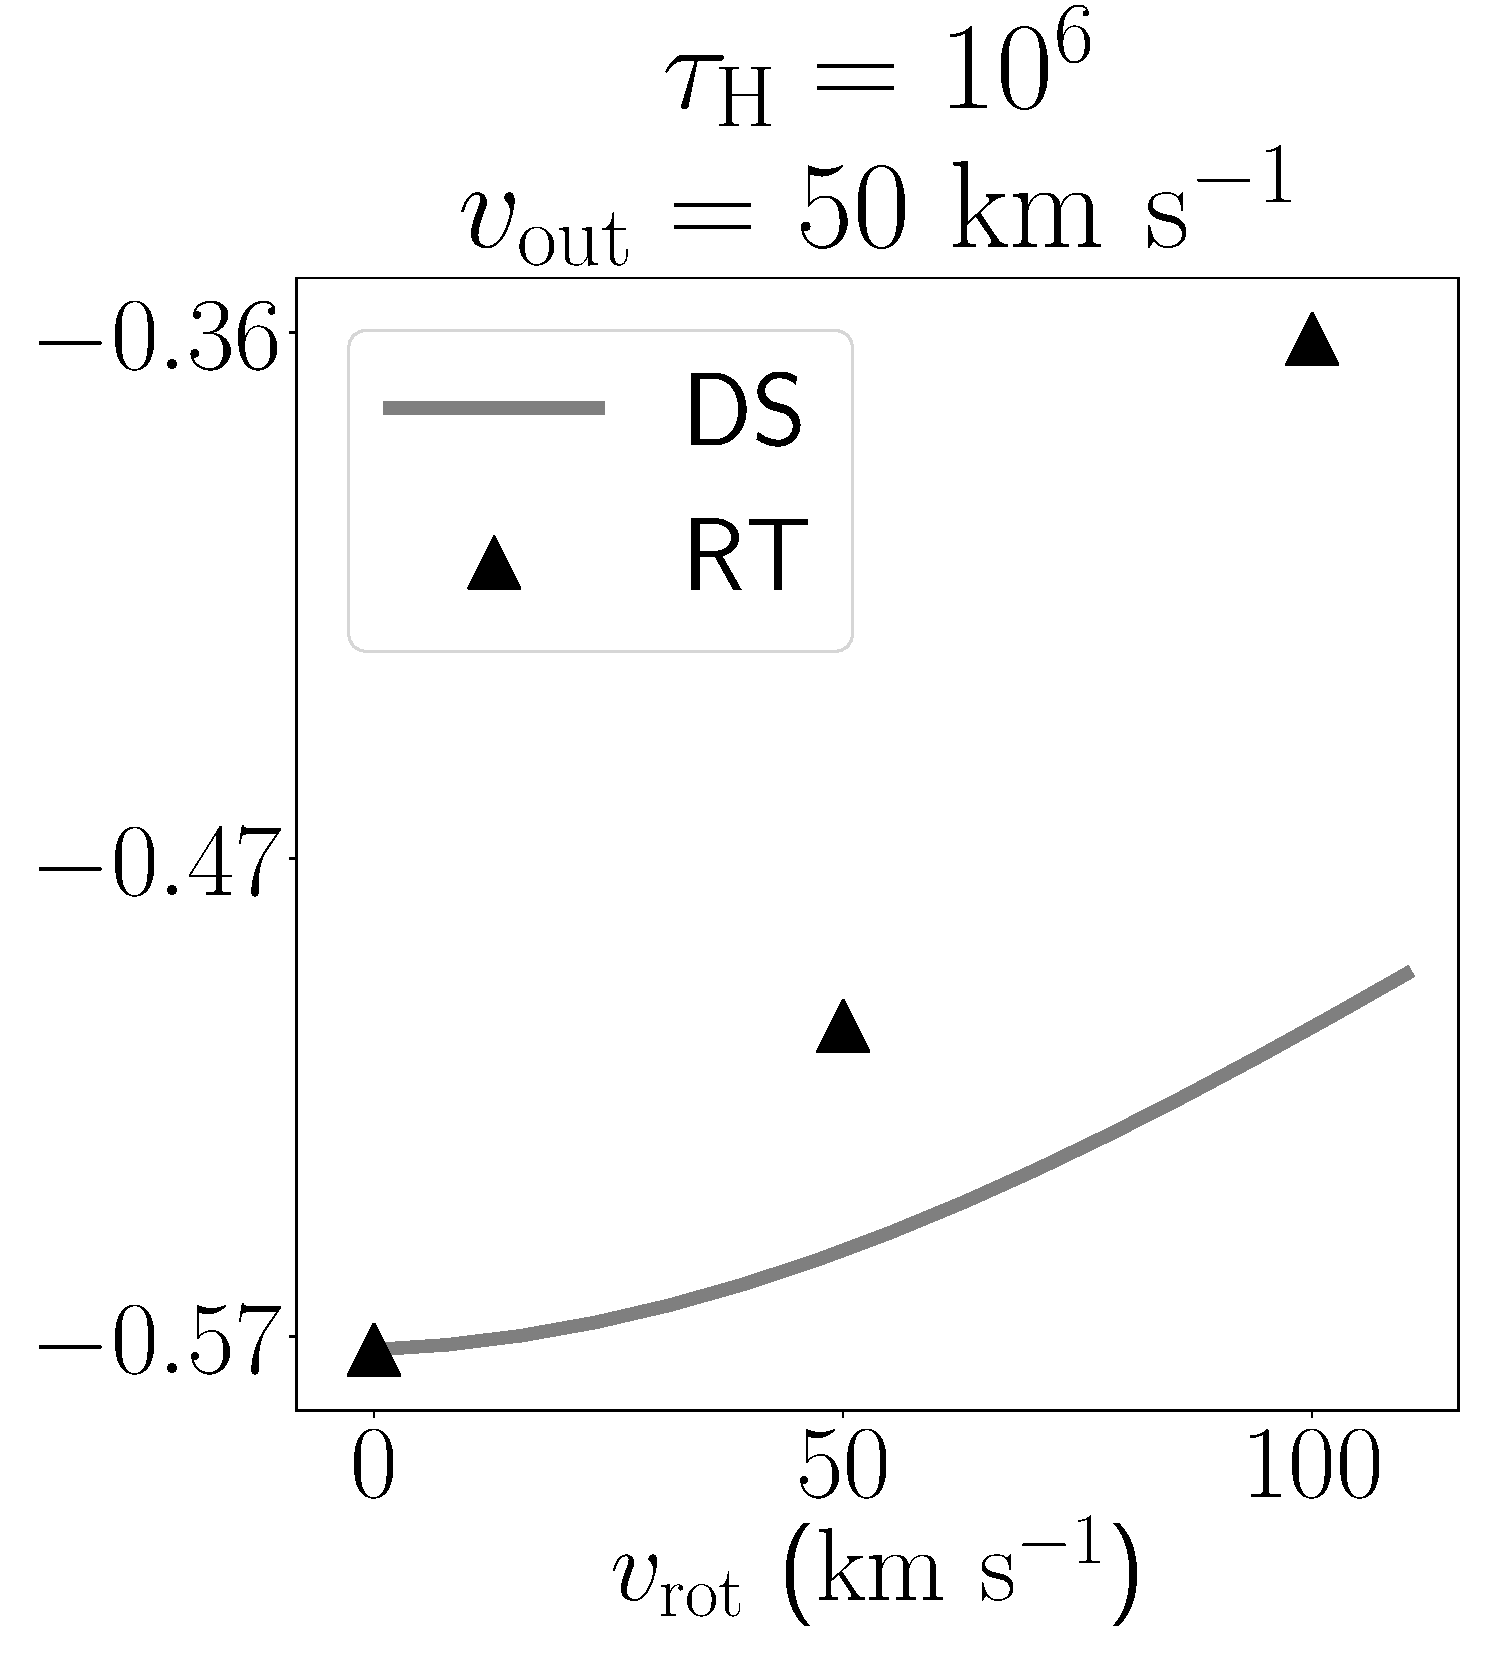
\includegraphics[height=0.27\textwidth]{./figures/results/line_characterization_skw_vout50_logtau6}
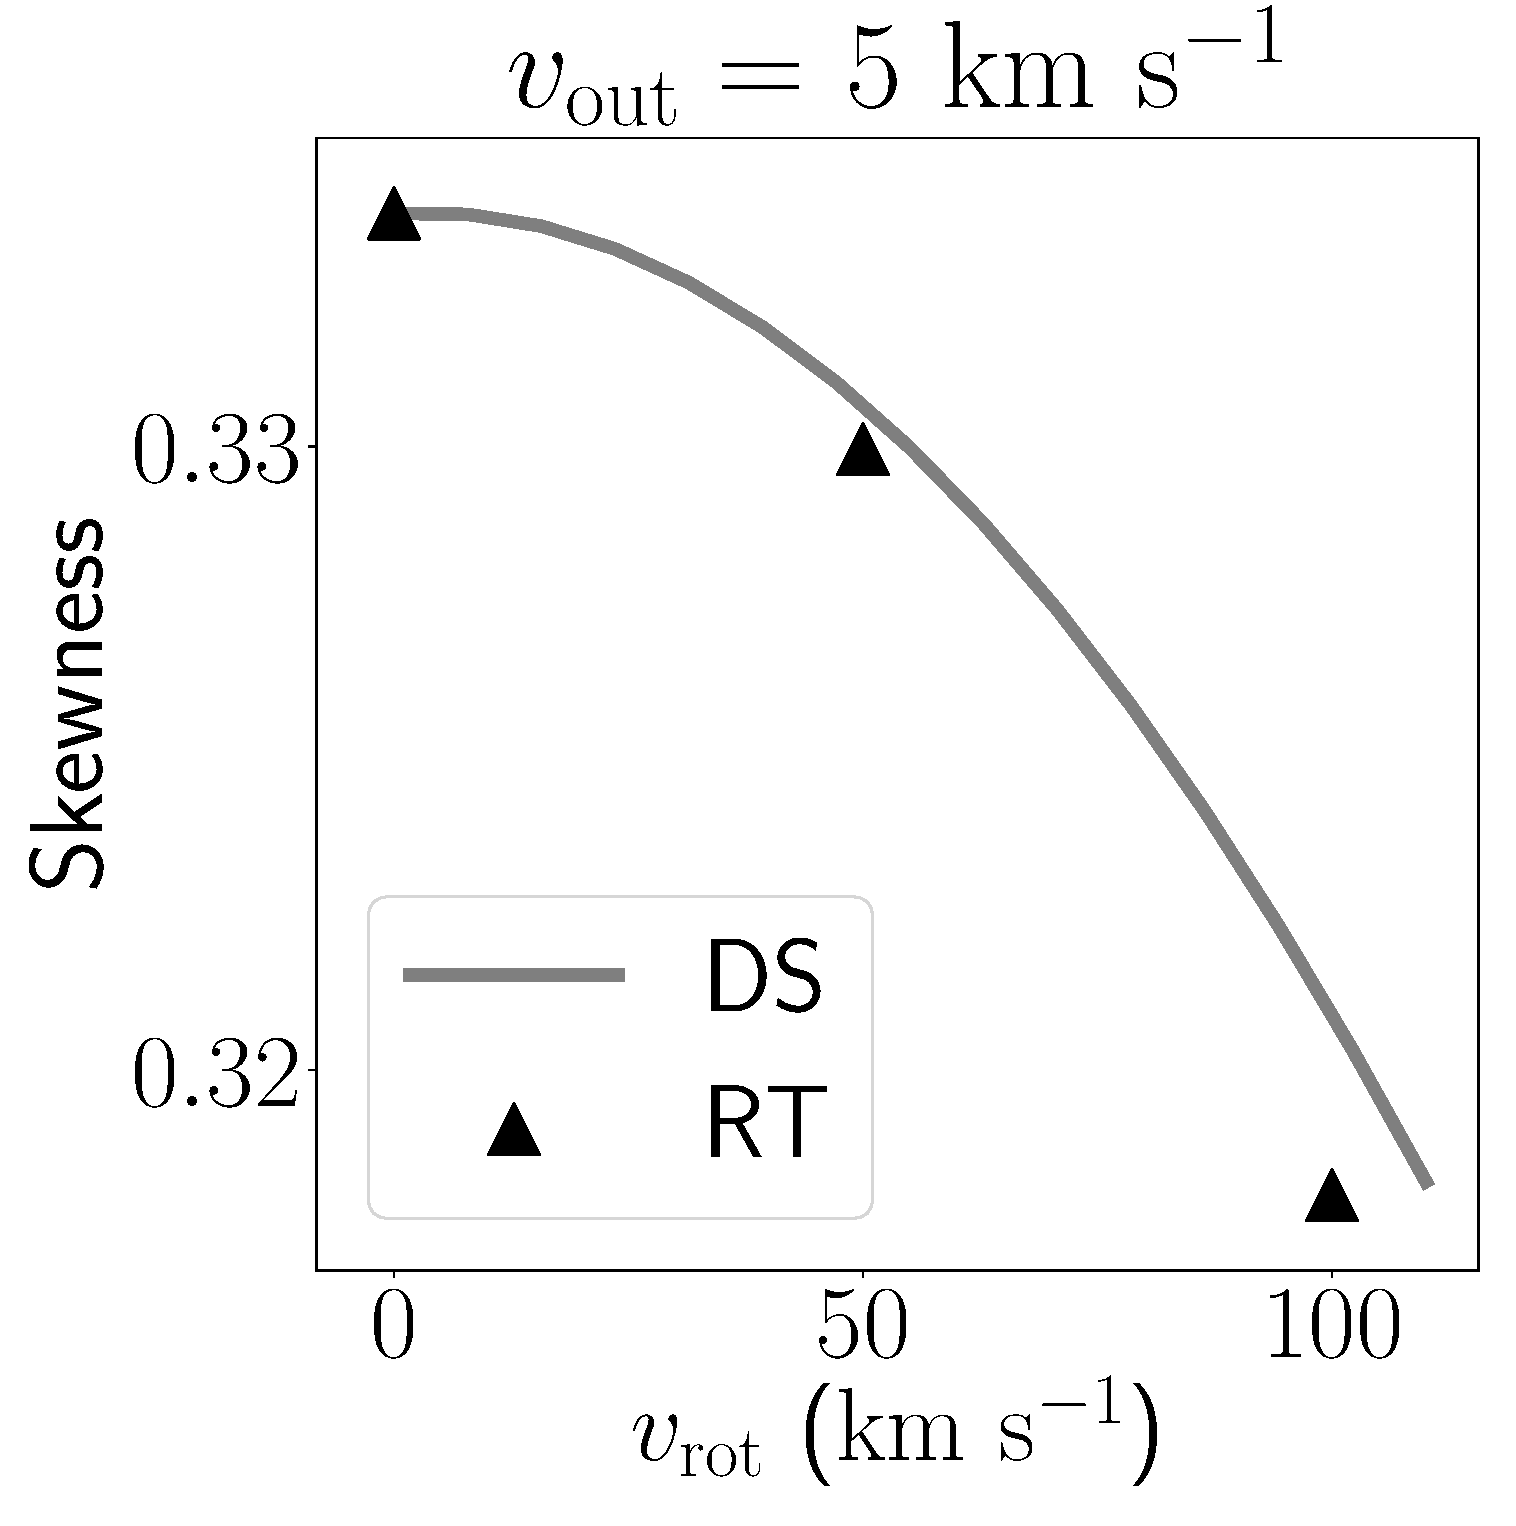
\includegraphics[height=0.27\textwidth]{./figures/results/line_characterization_skw_vout5_logtau7}
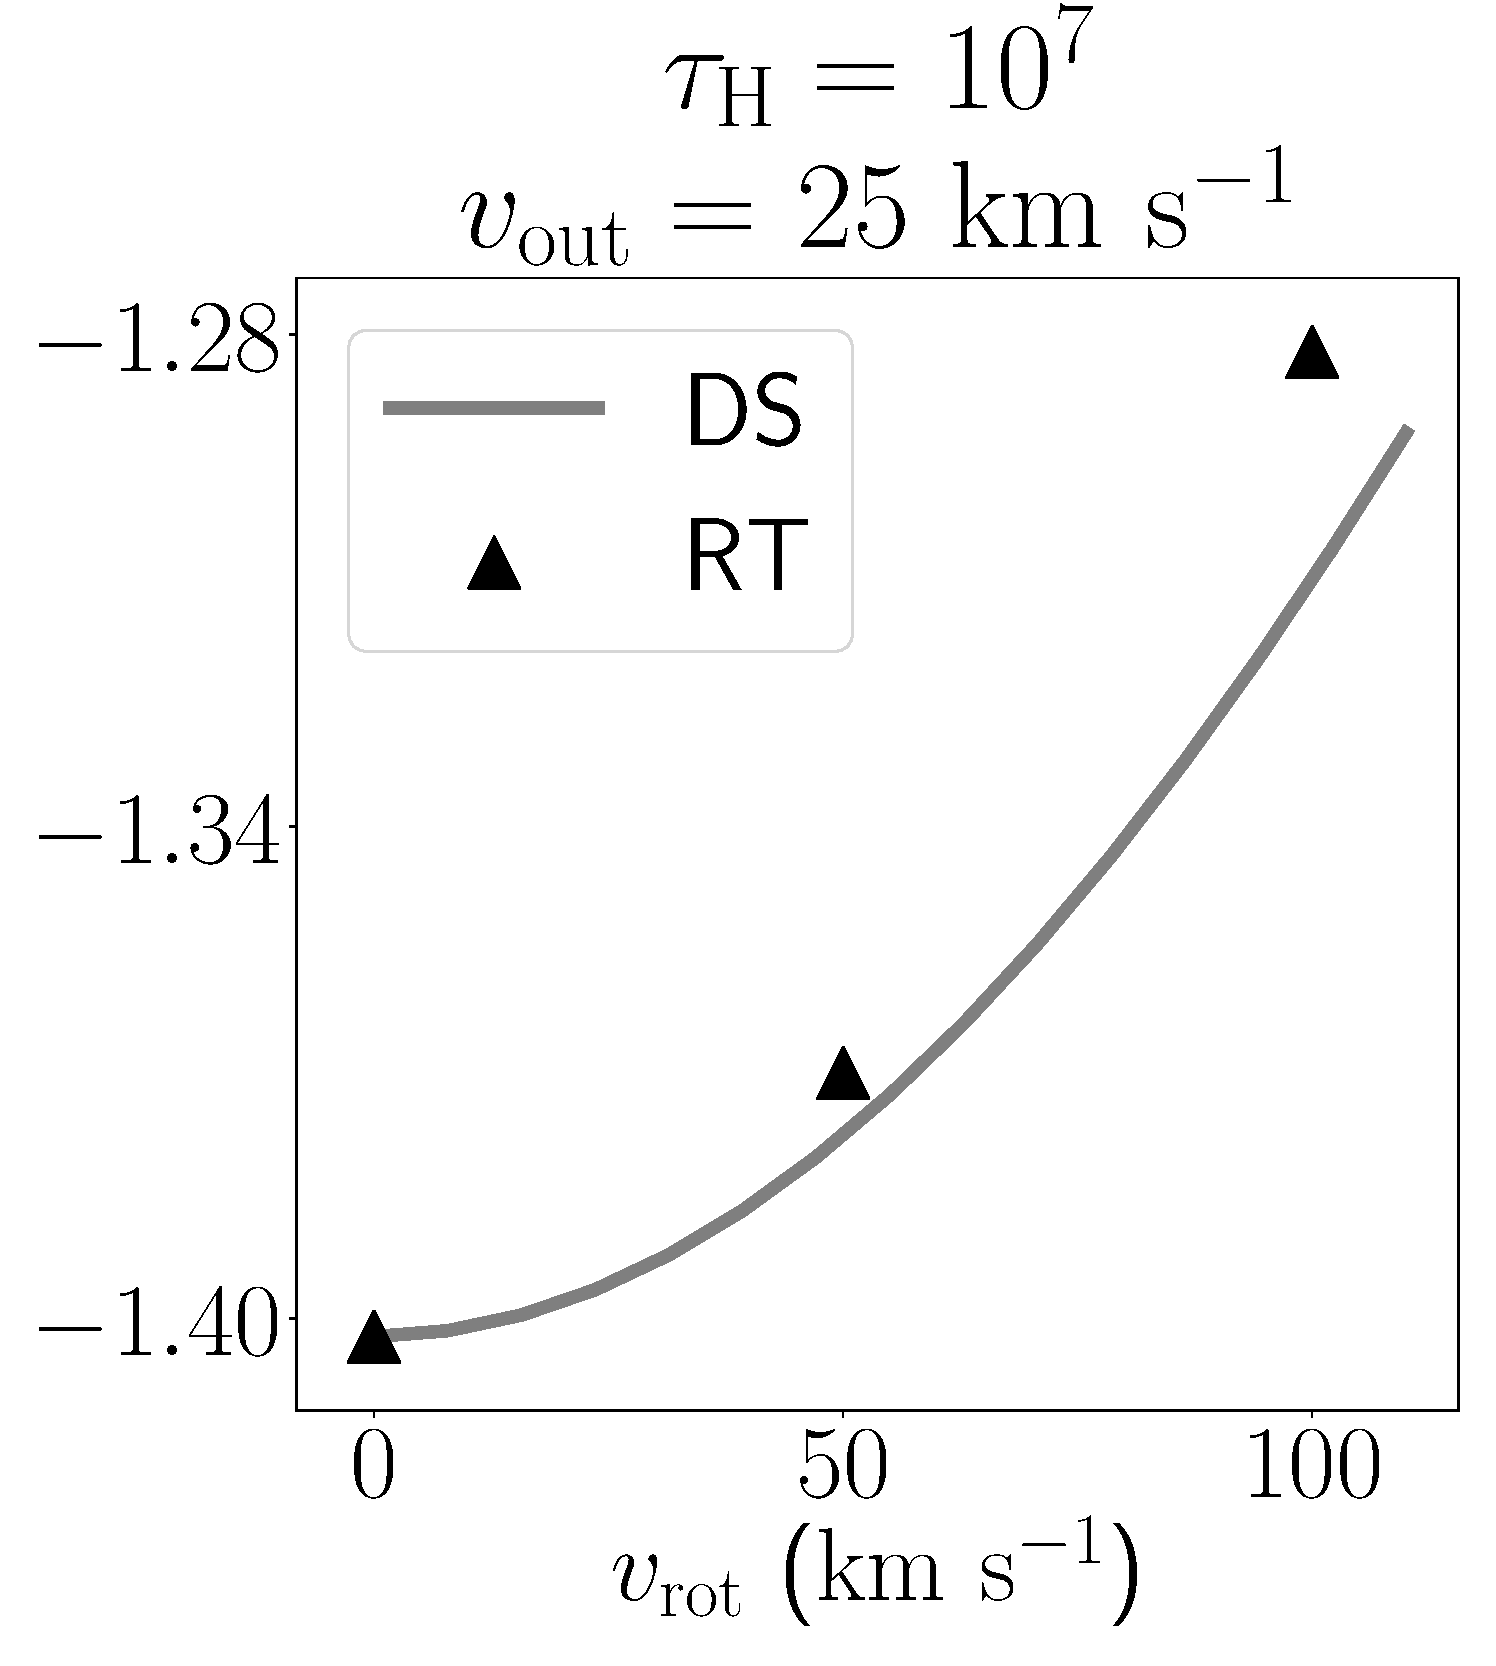
\includegraphics[height=0.27\textwidth]{./figures/results/line_characterization_skw_vout25_logtau7}
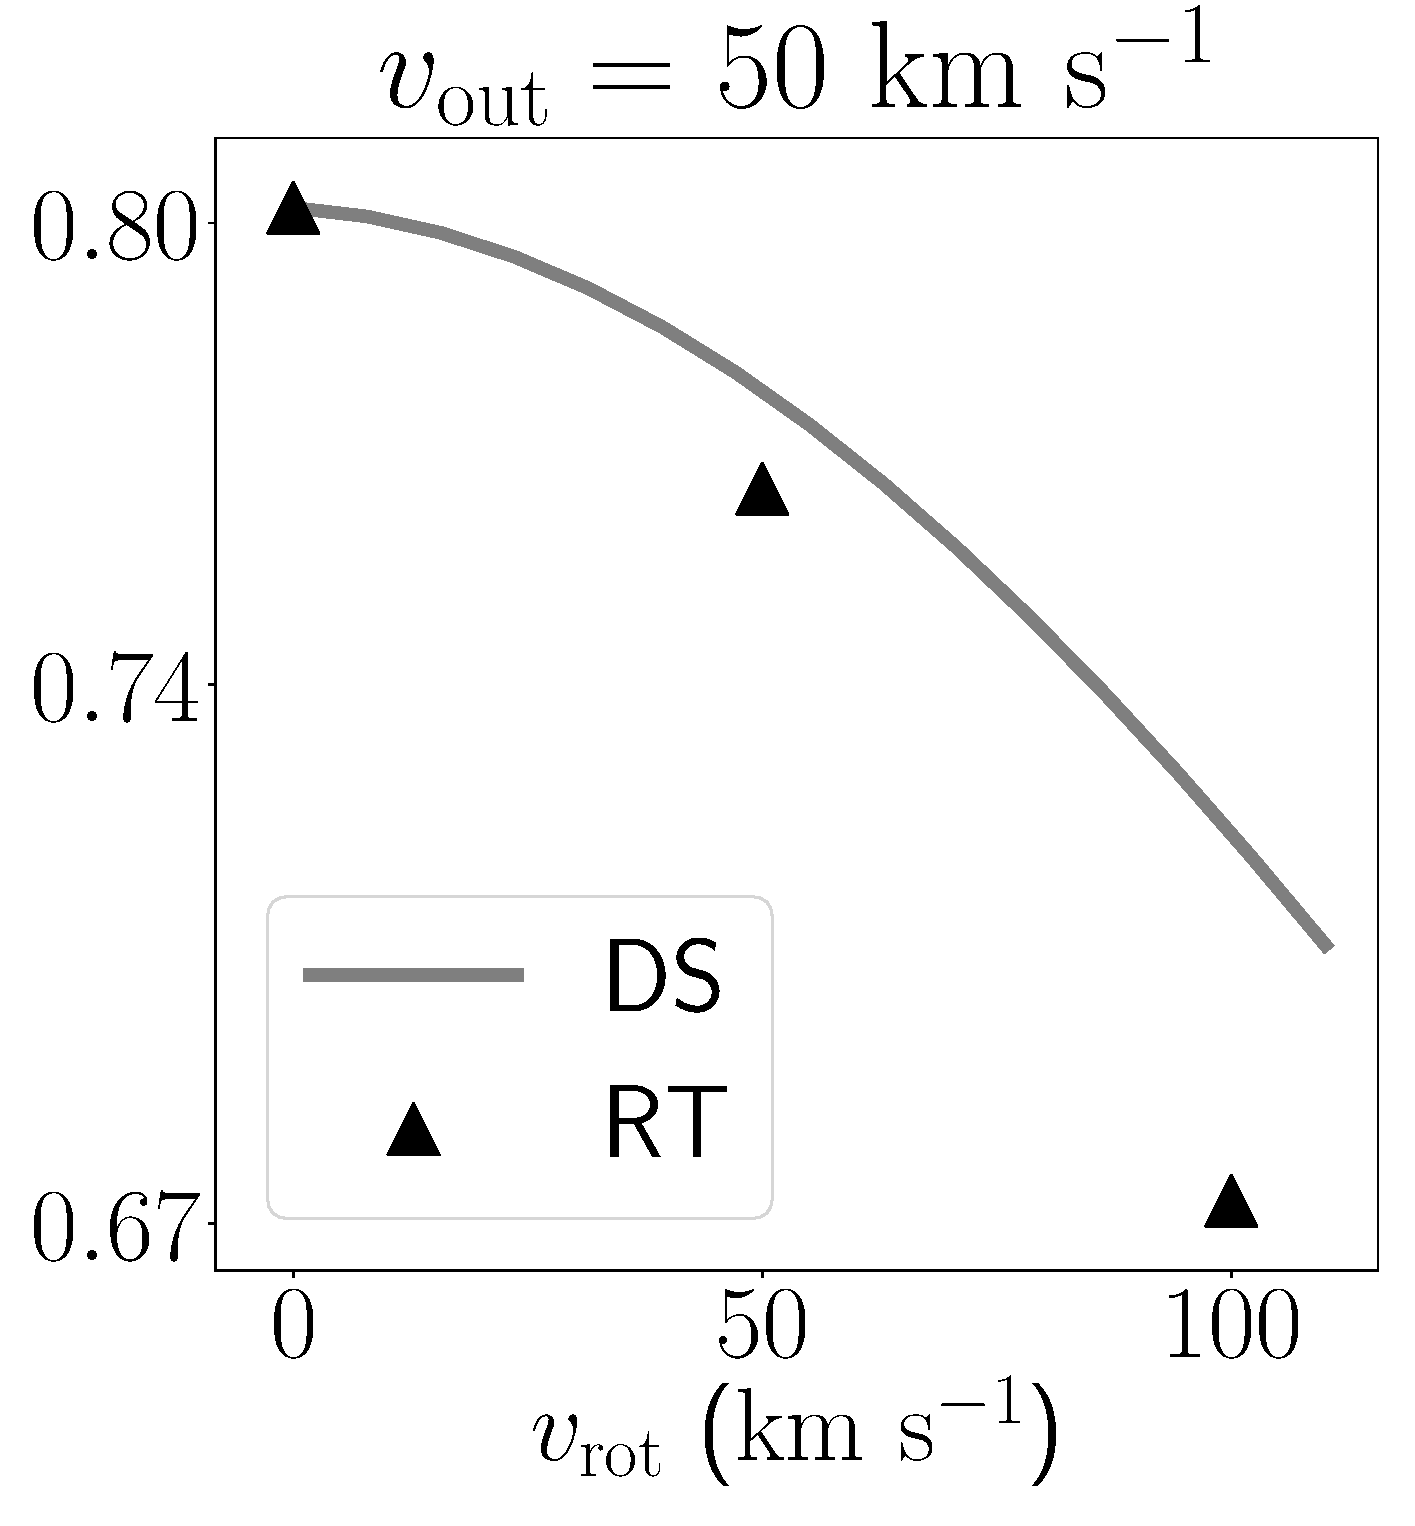
\includegraphics[height=0.27\textwidth]{./figures/results/line_characterization_skw_vout50_logtau7}
\end{center}
\caption{\textbf{Skewness trends.} Results for all the
  Radiative Transfer simulations (in triangles) compares against the
  Doppler Shift model (lines).
  Follows the same layout as Figure \ref{fig:standard_deviation}. 
  \label{fig:skewness}}
\end{figure*}

\begin{figure*}
\begin{center}
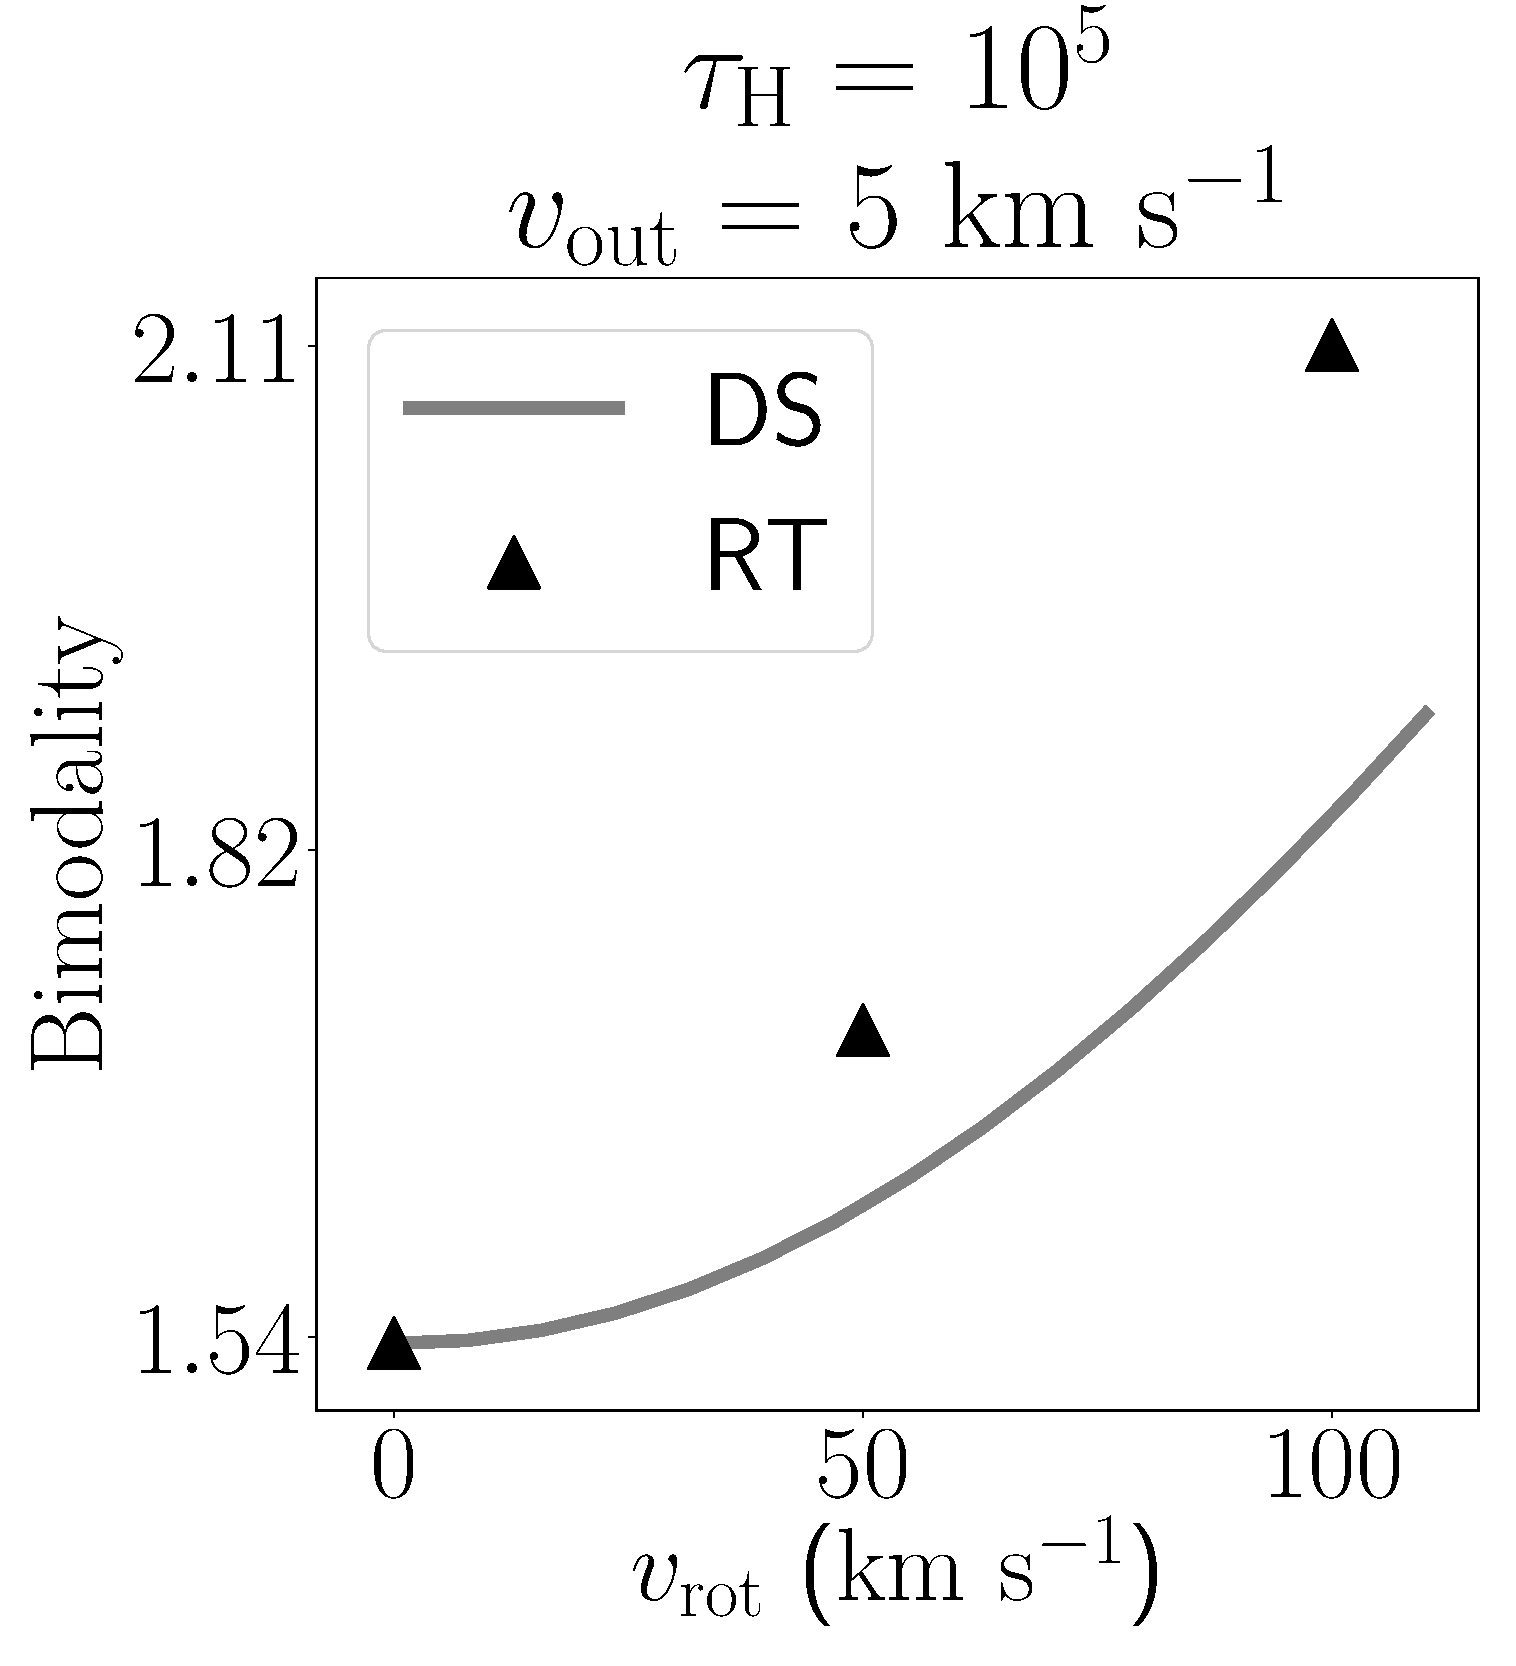
\includegraphics[height=0.28\textwidth]{./figures/results/line_characterization_bi_vout5_logtau5}
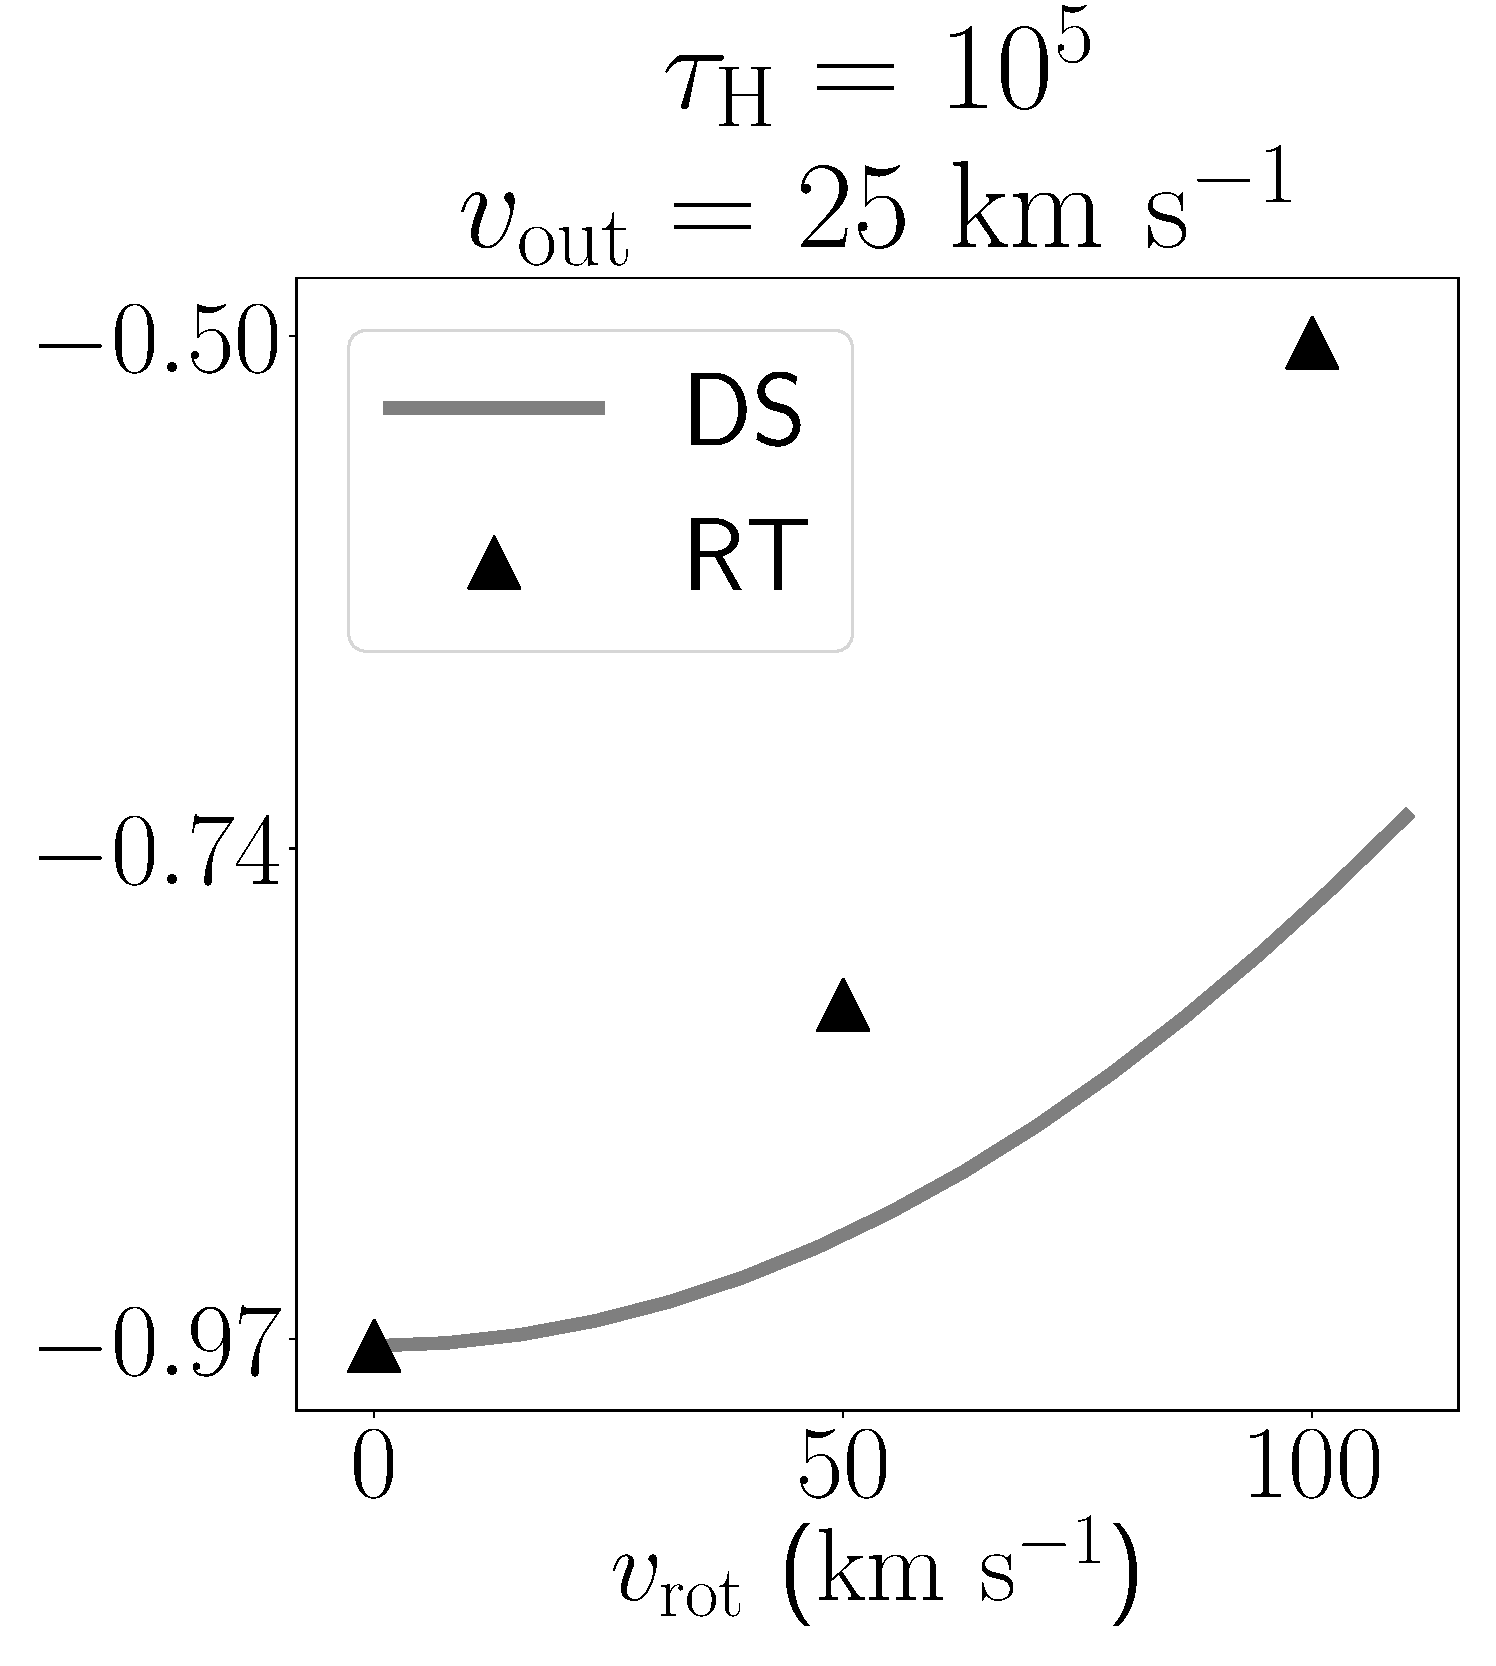
\includegraphics[height=0.28\textwidth]{./figures/results/line_characterization_bi_vout25_logtau5}
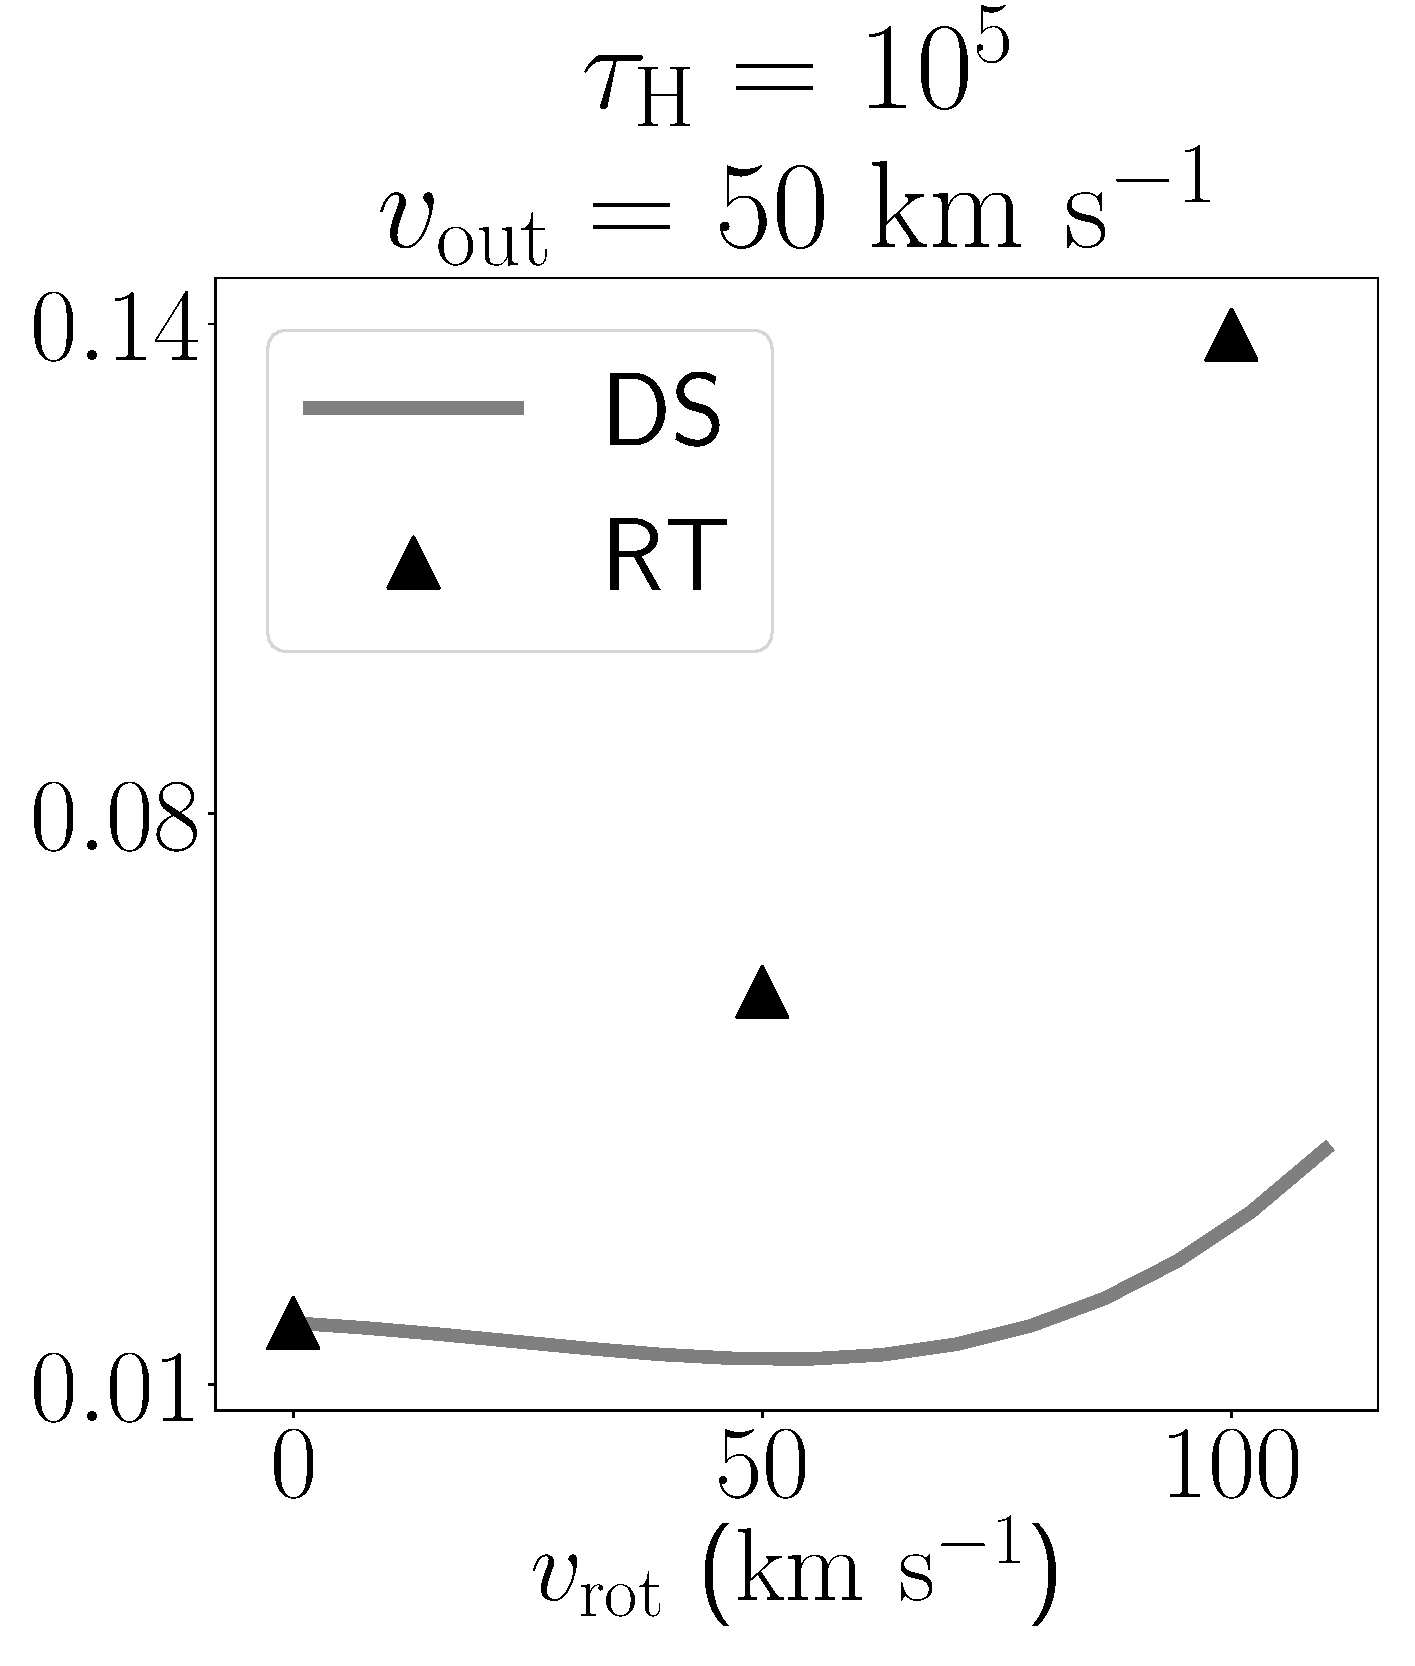
\includegraphics[height=0.28\textwidth]{./figures/results/line_characterization_bi_vout50_logtau5}
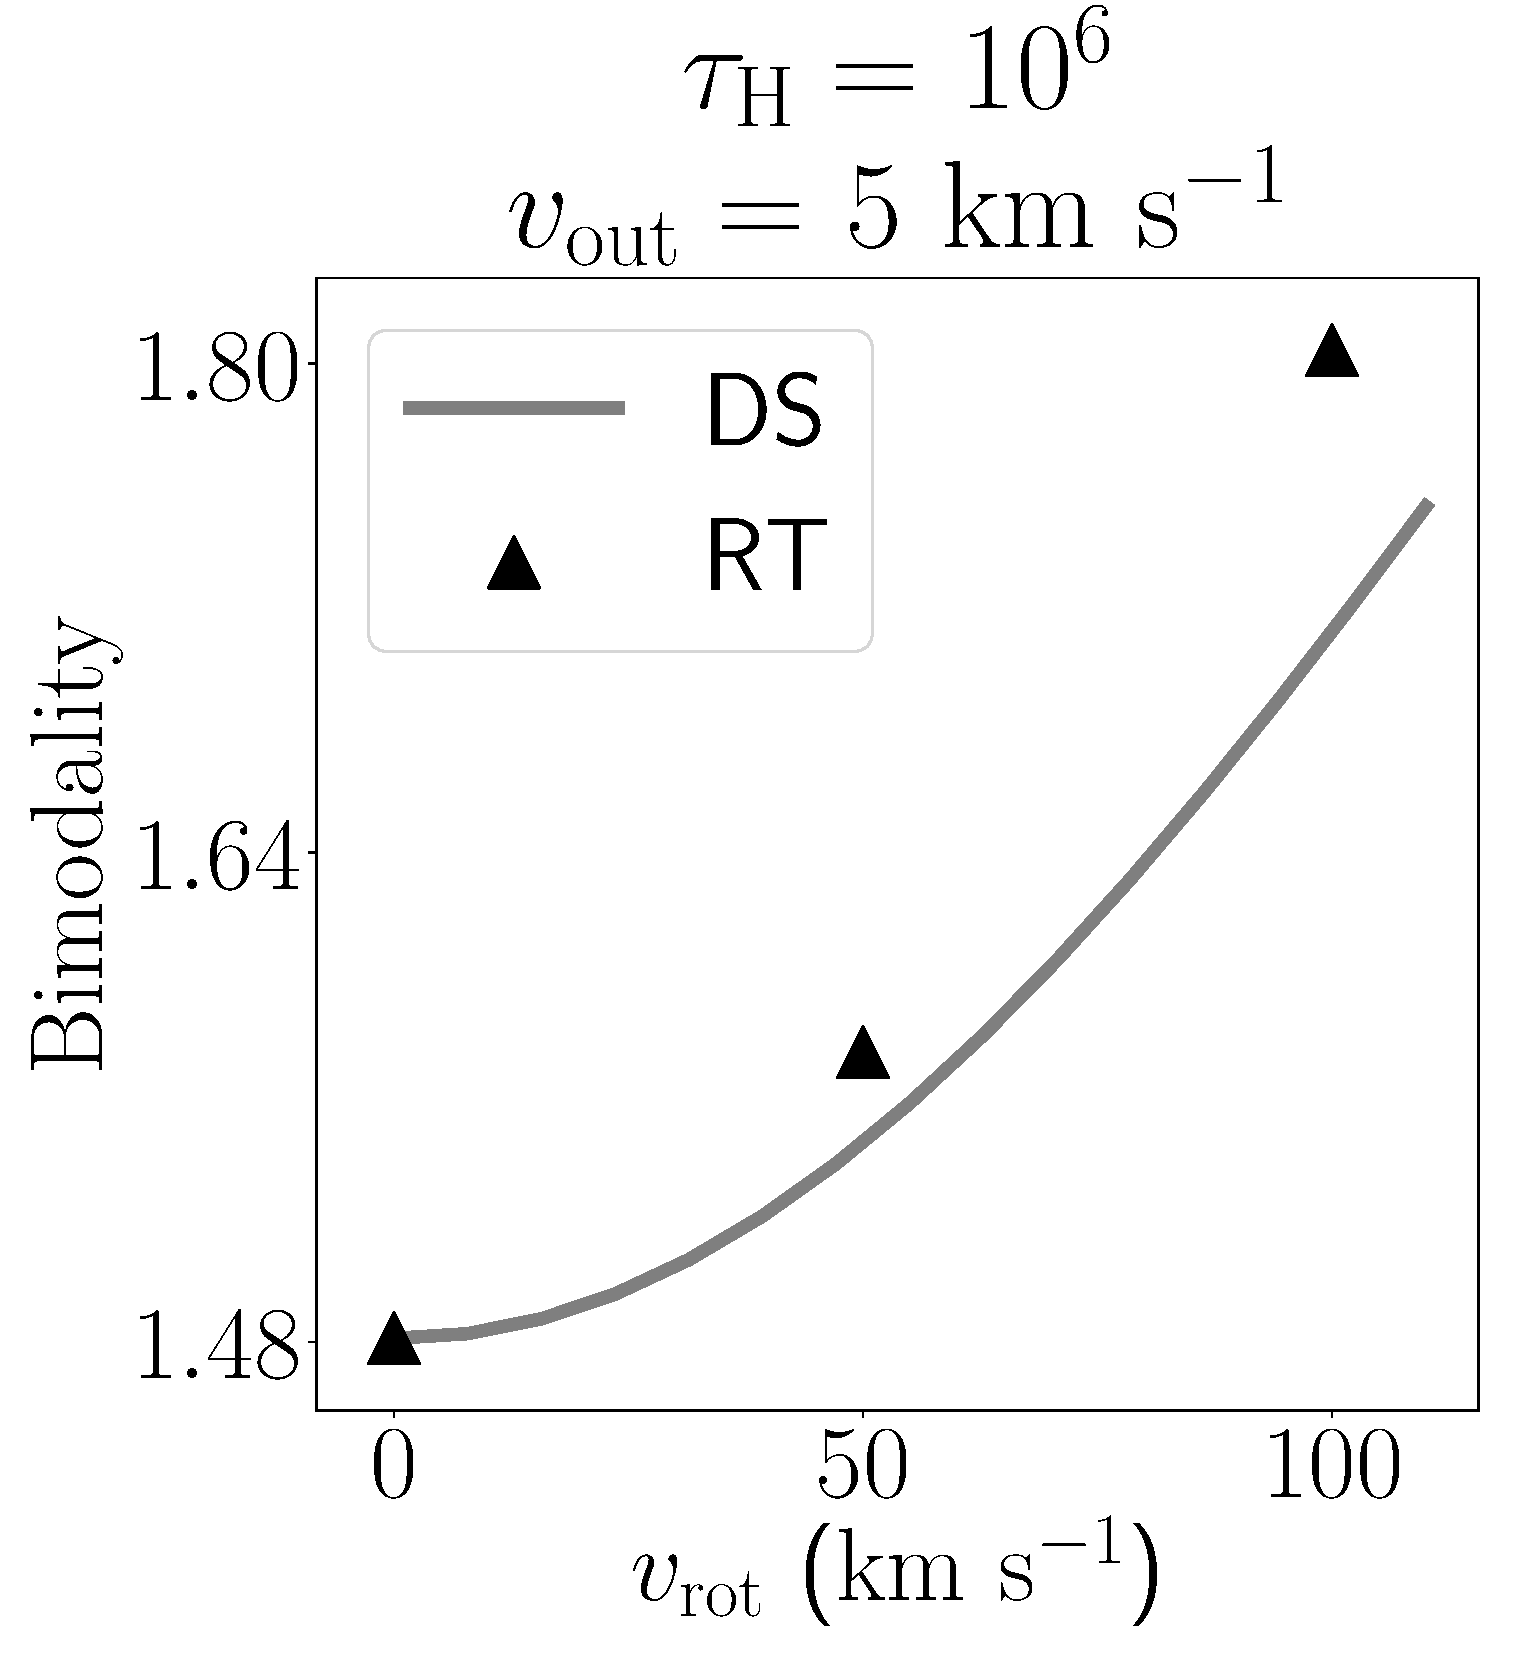
\includegraphics[height=0.28\textwidth]{./figures/results/line_characterization_bi_vout5_logtau6}
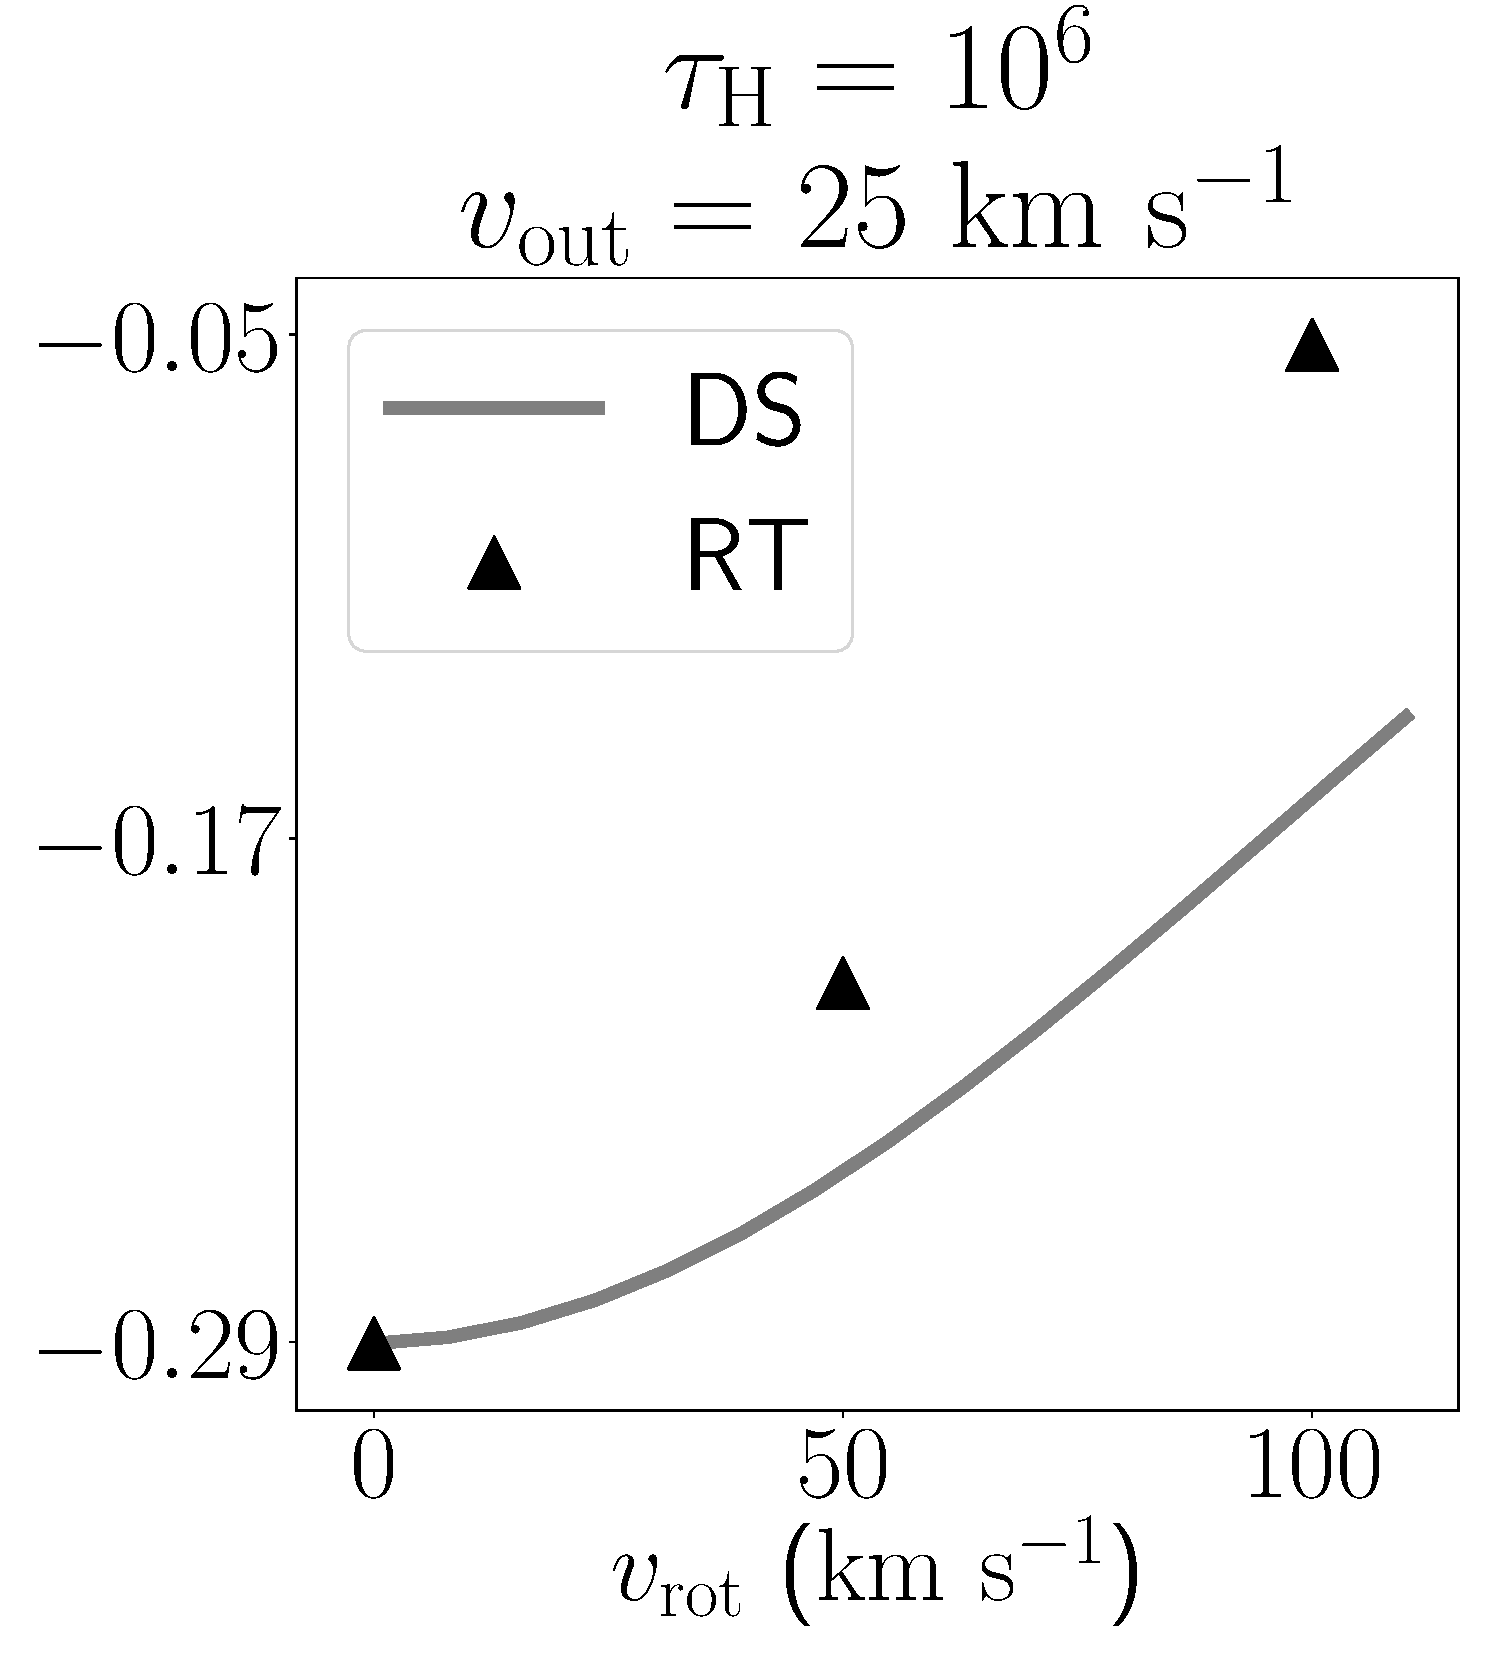
\includegraphics[height=0.28\textwidth]{./figures/results/line_characterization_bi_vout25_logtau6}
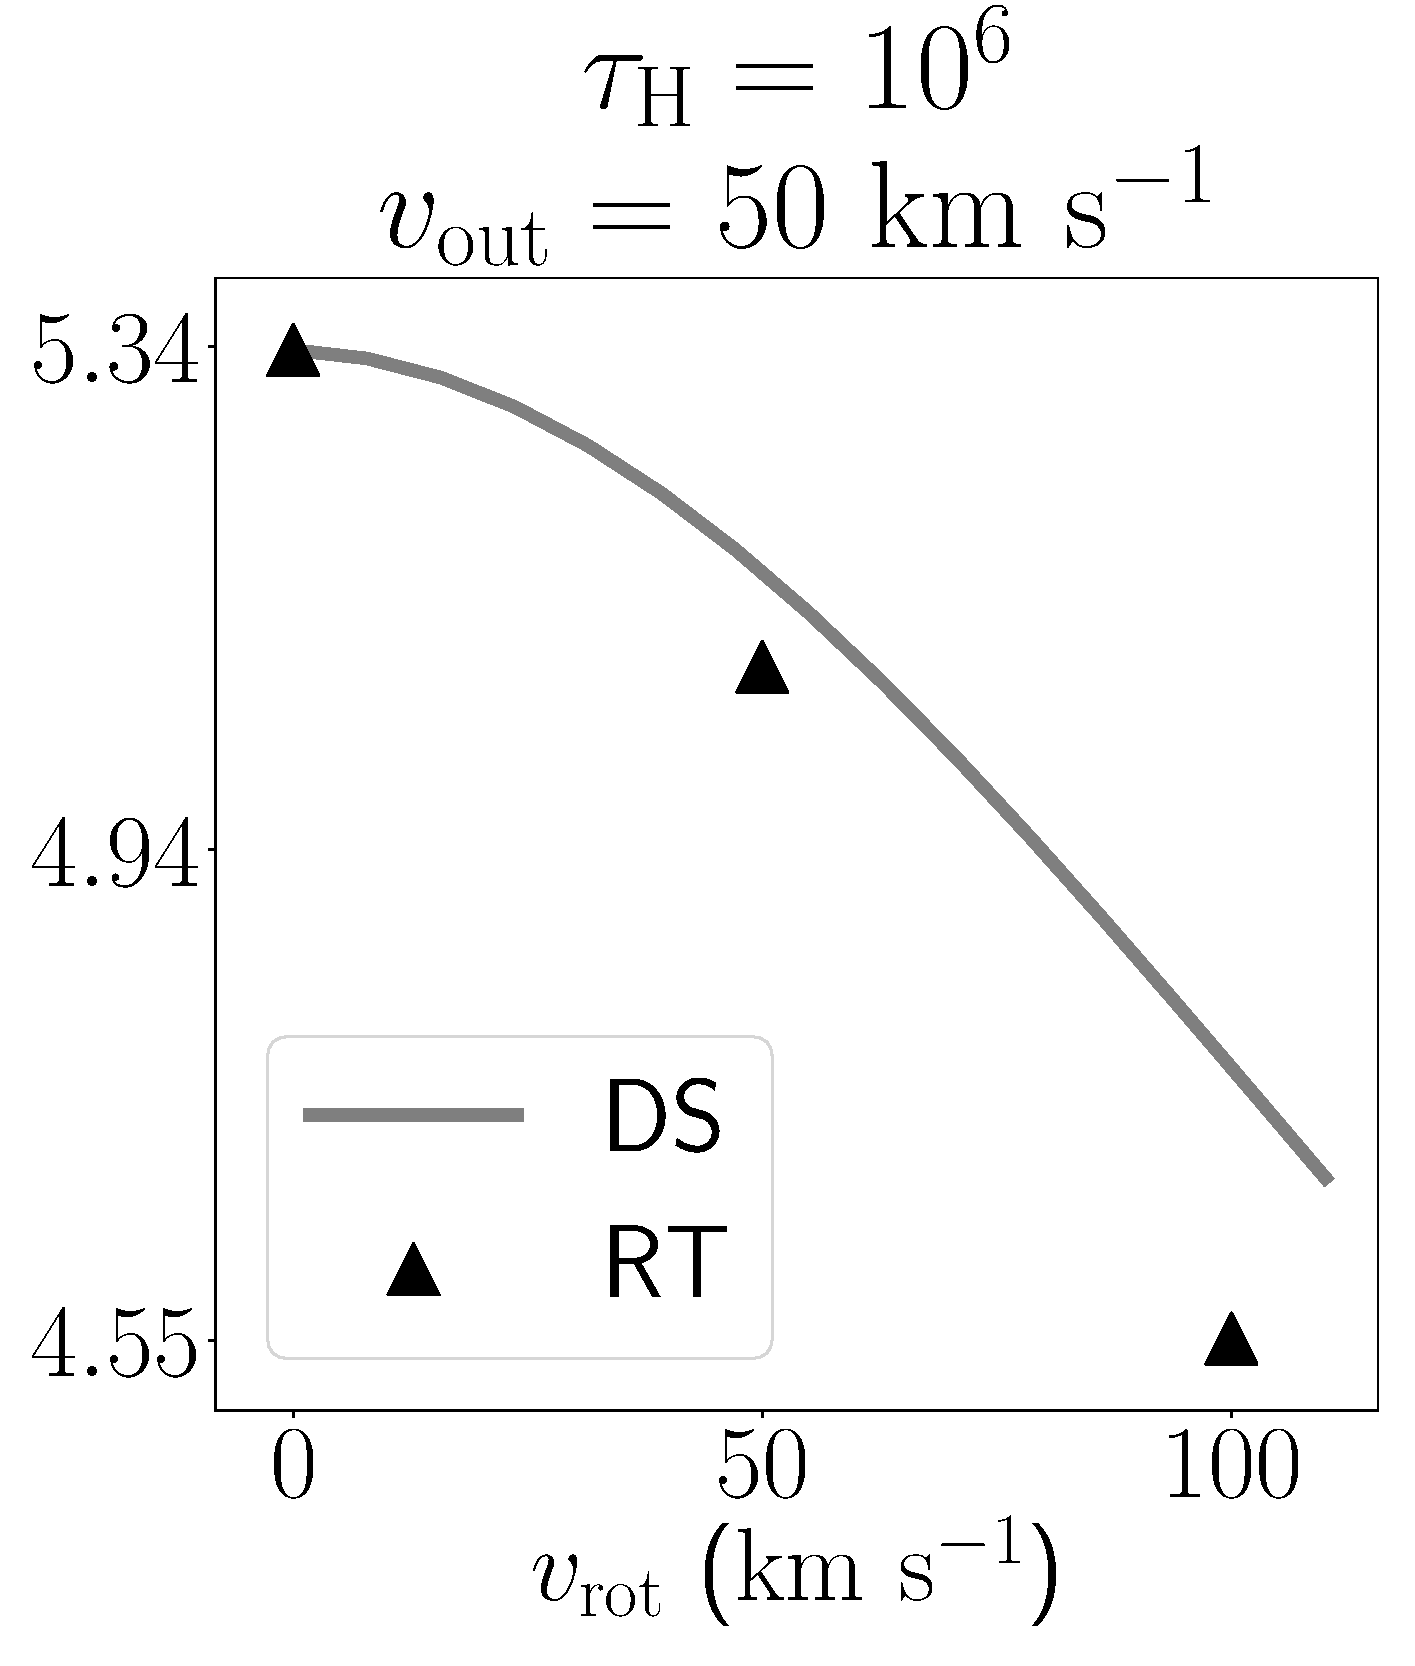
\includegraphics[height=0.28\textwidth]{./figures/results/line_characterization_bi_vout50_logtau6}
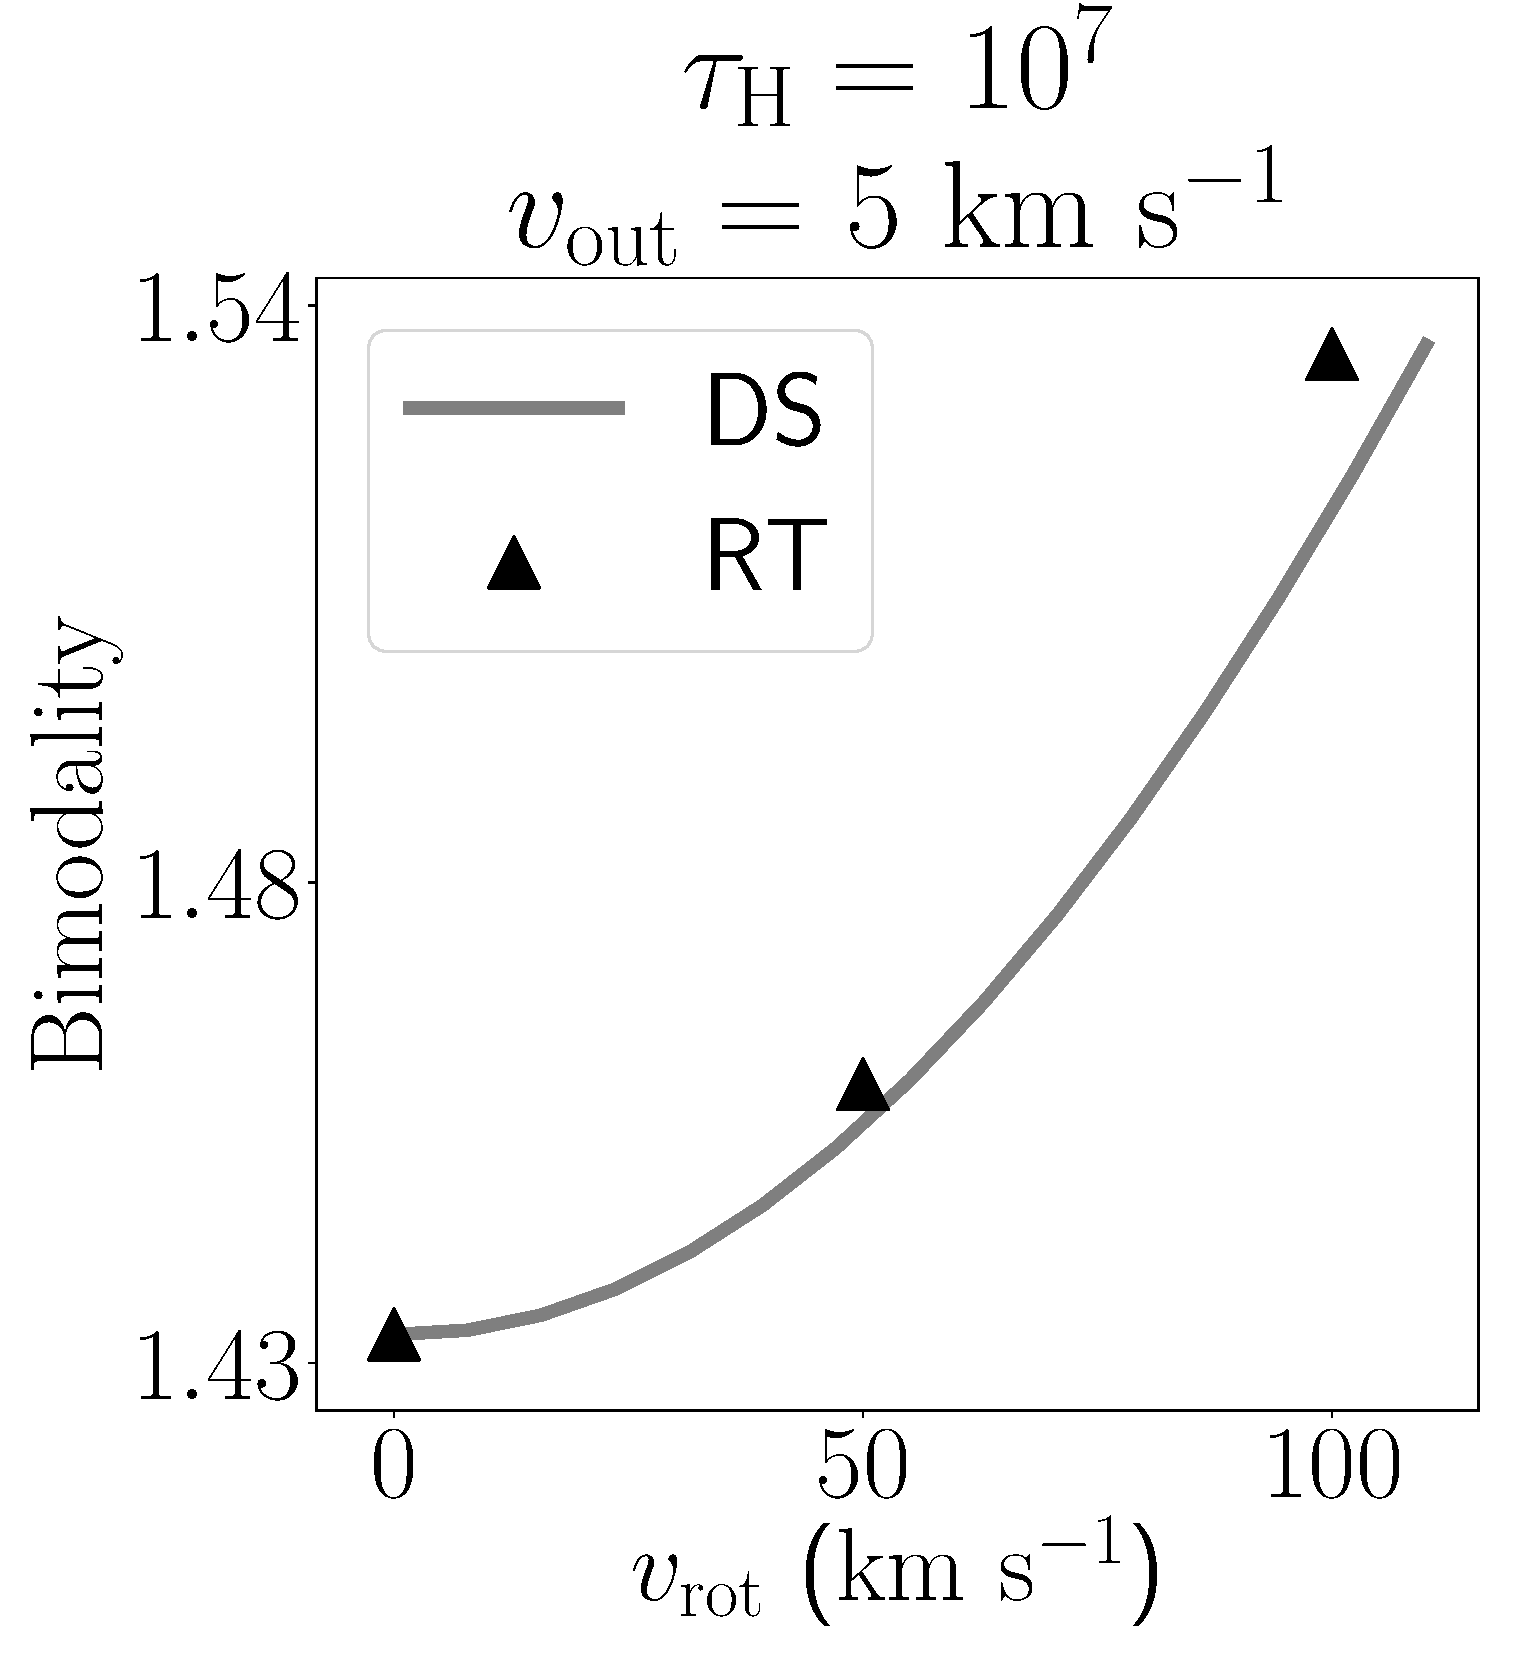
\includegraphics[height=0.28\textwidth]{./figures/results/line_characterization_bi_vout5_logtau7}
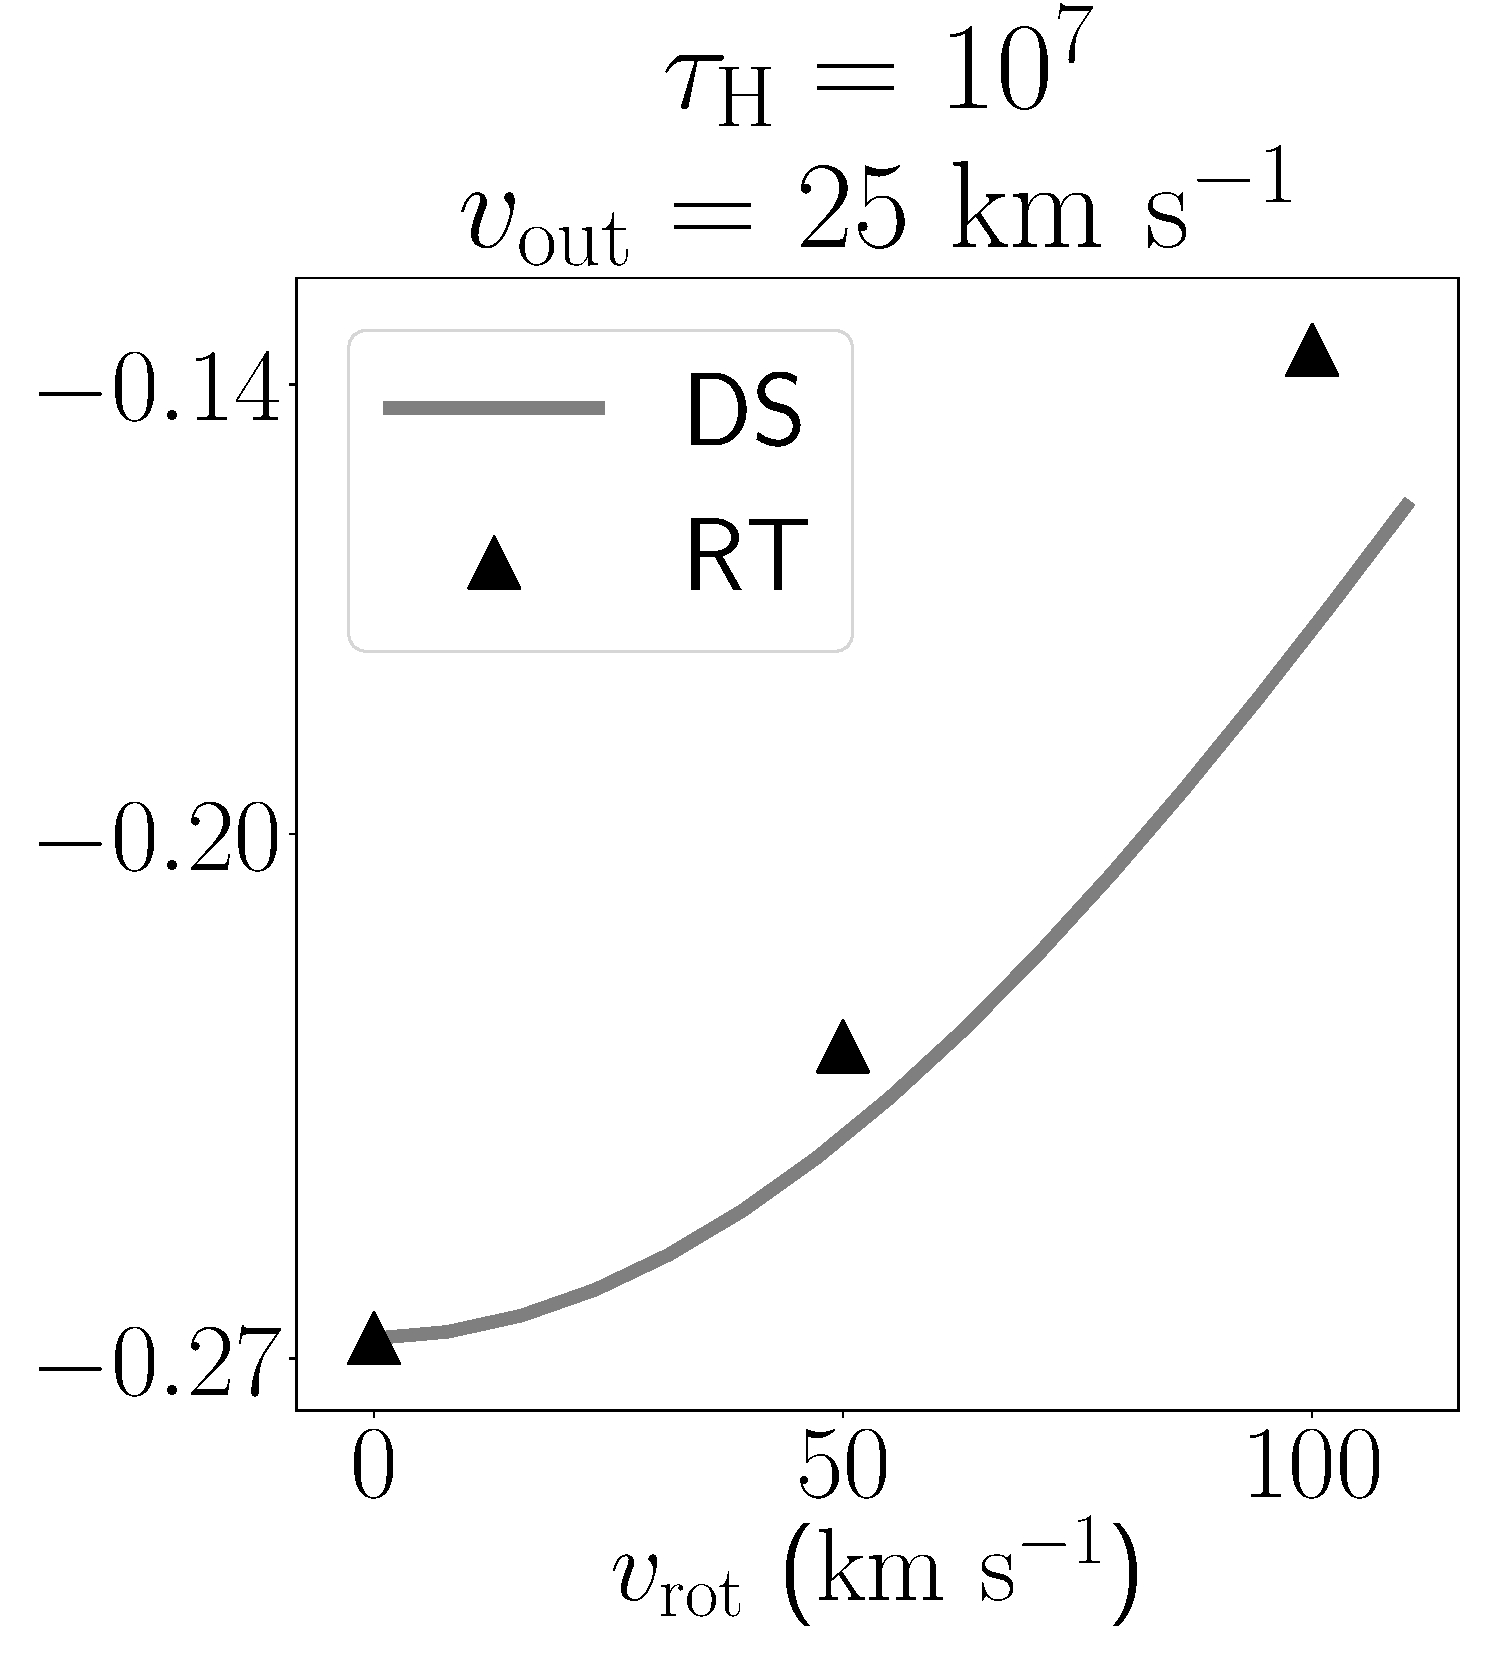
\includegraphics[height=0.28\textwidth]{./figures/results/line_characterization_bi_vout25_logtau7}
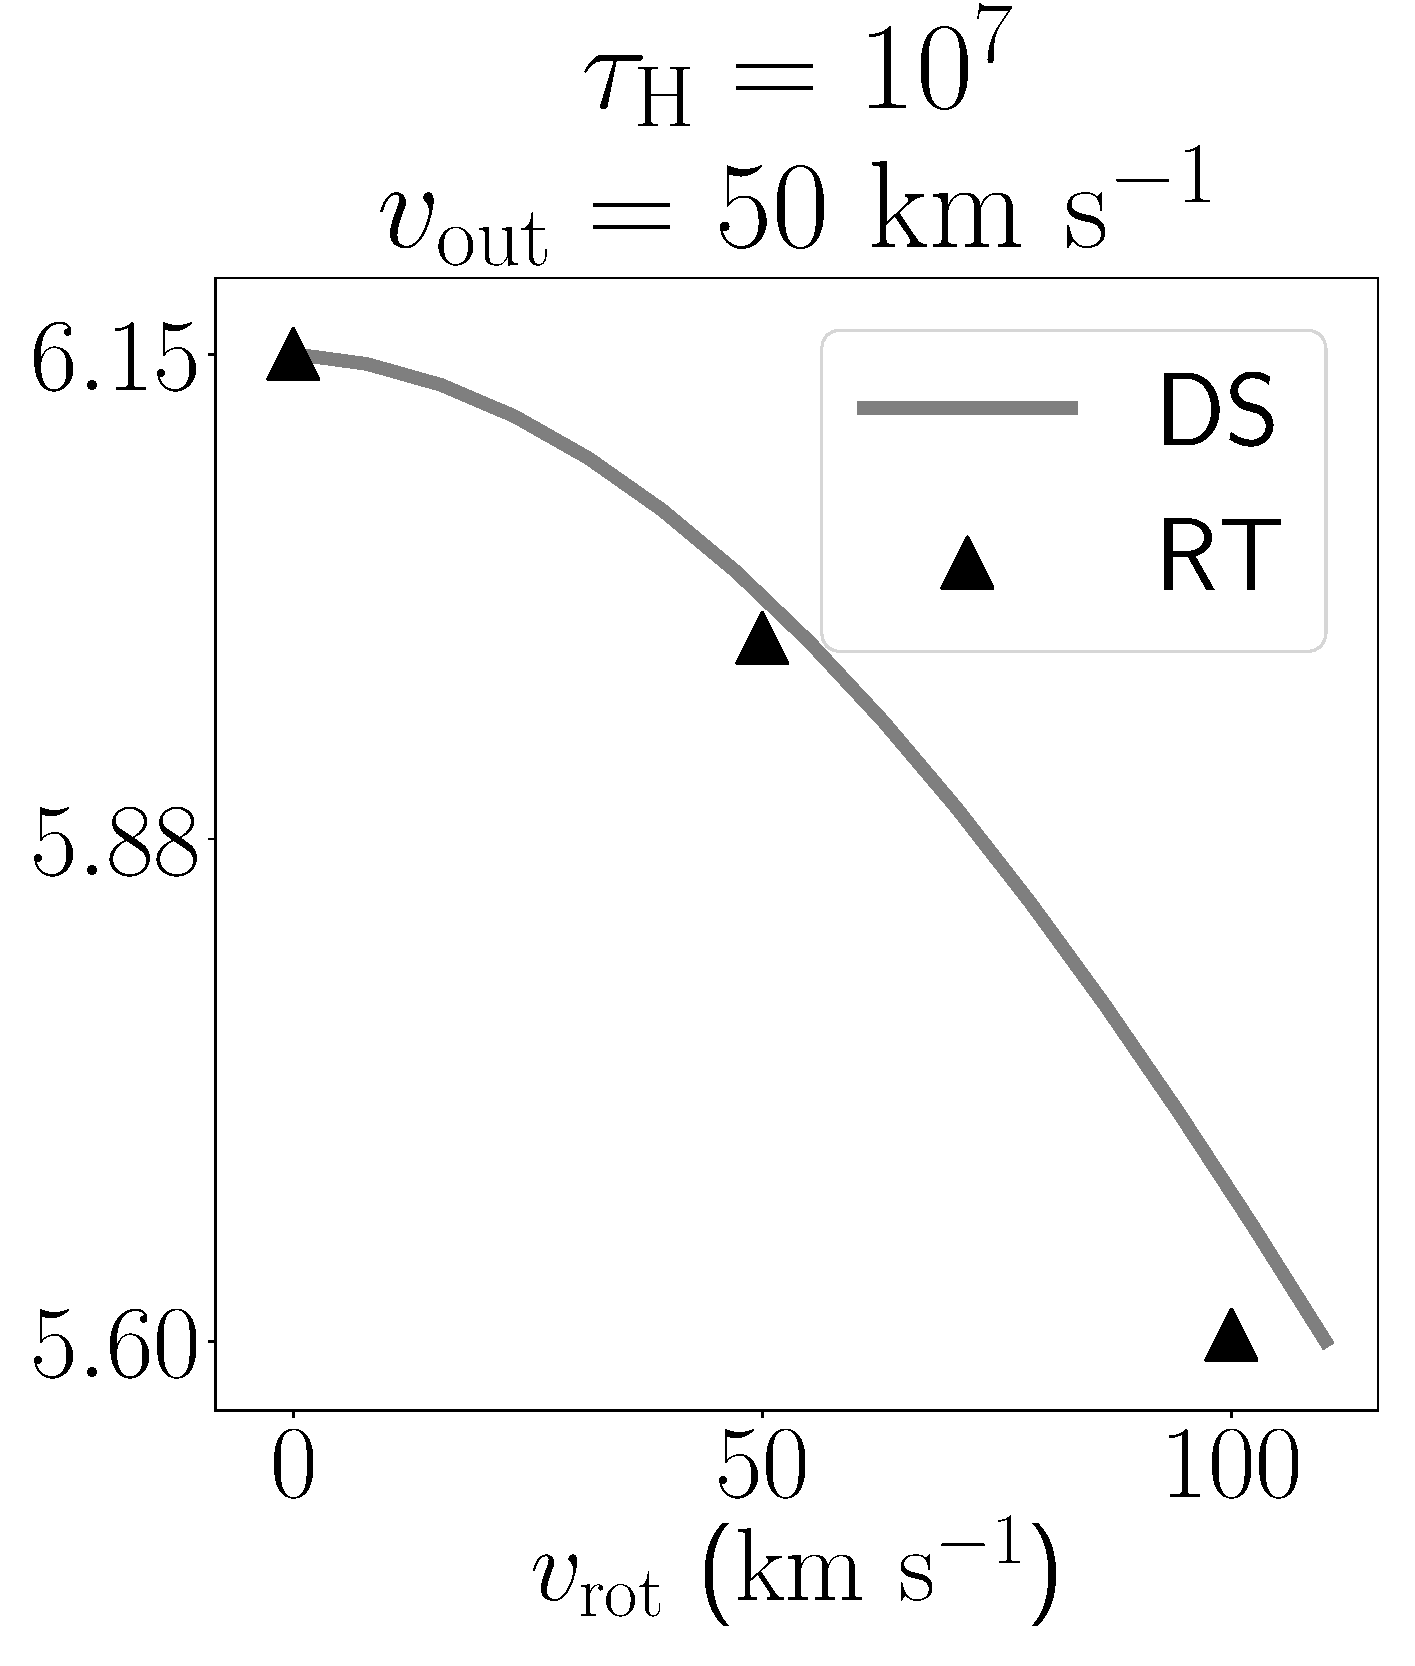
\includegraphics[height=0.28\textwidth]{./figures/results/line_characterization_bi_vout50_logtau7}
\end{center}
\caption{\textbf{Bimodality trends.} Results for all the
  Radiative Transfer simulations (in triangles) compares against the
  Doppler Shift model (lines). 
  Follows the same layout as Figure \ref{fig:standard_deviation}. 
  \label{fig:bimodality}}
\end{figure*}


\begin{figure*}
\begin{center}
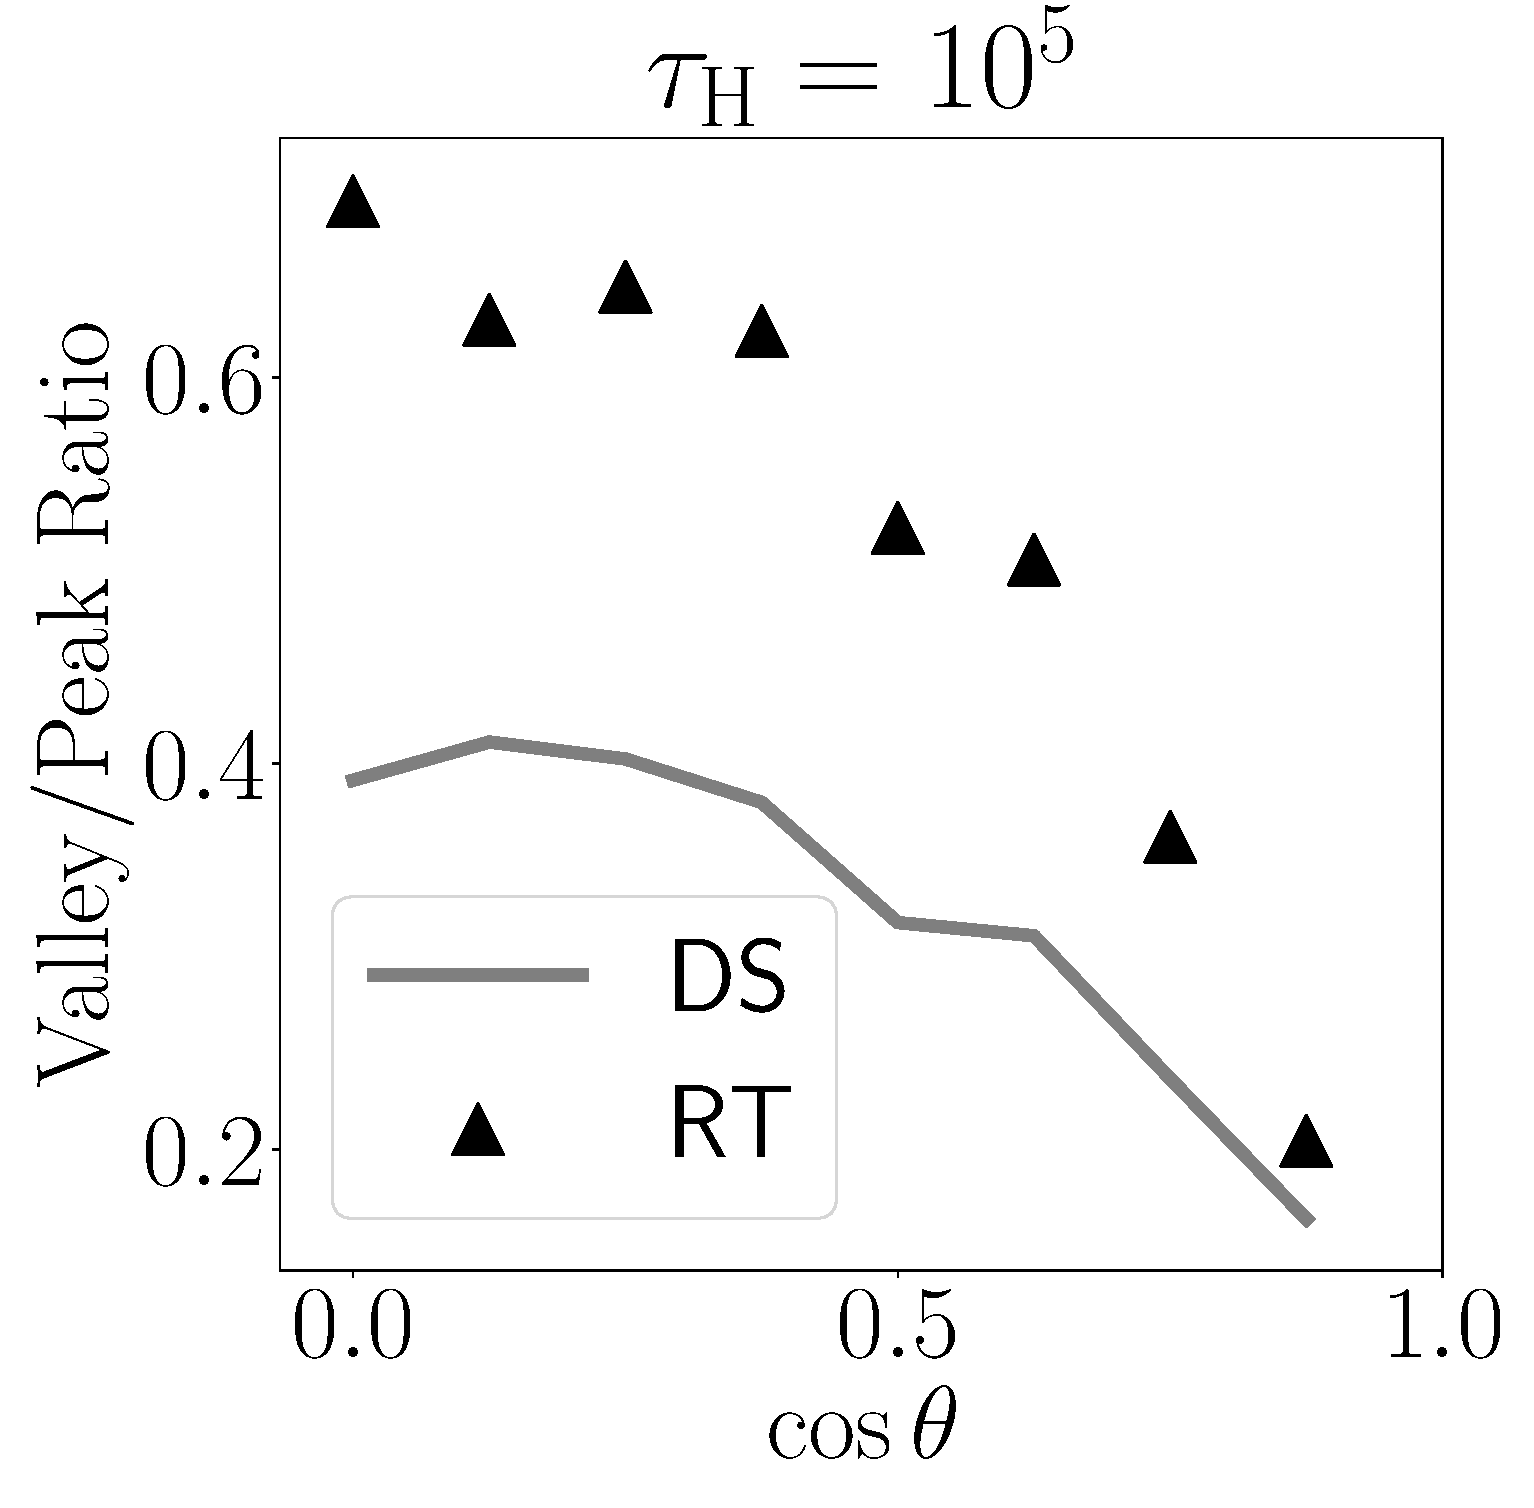
\includegraphics[height=0.28\textwidth]{./figures/results/line_characterization_vi_vout5_vrot100_logtau5}
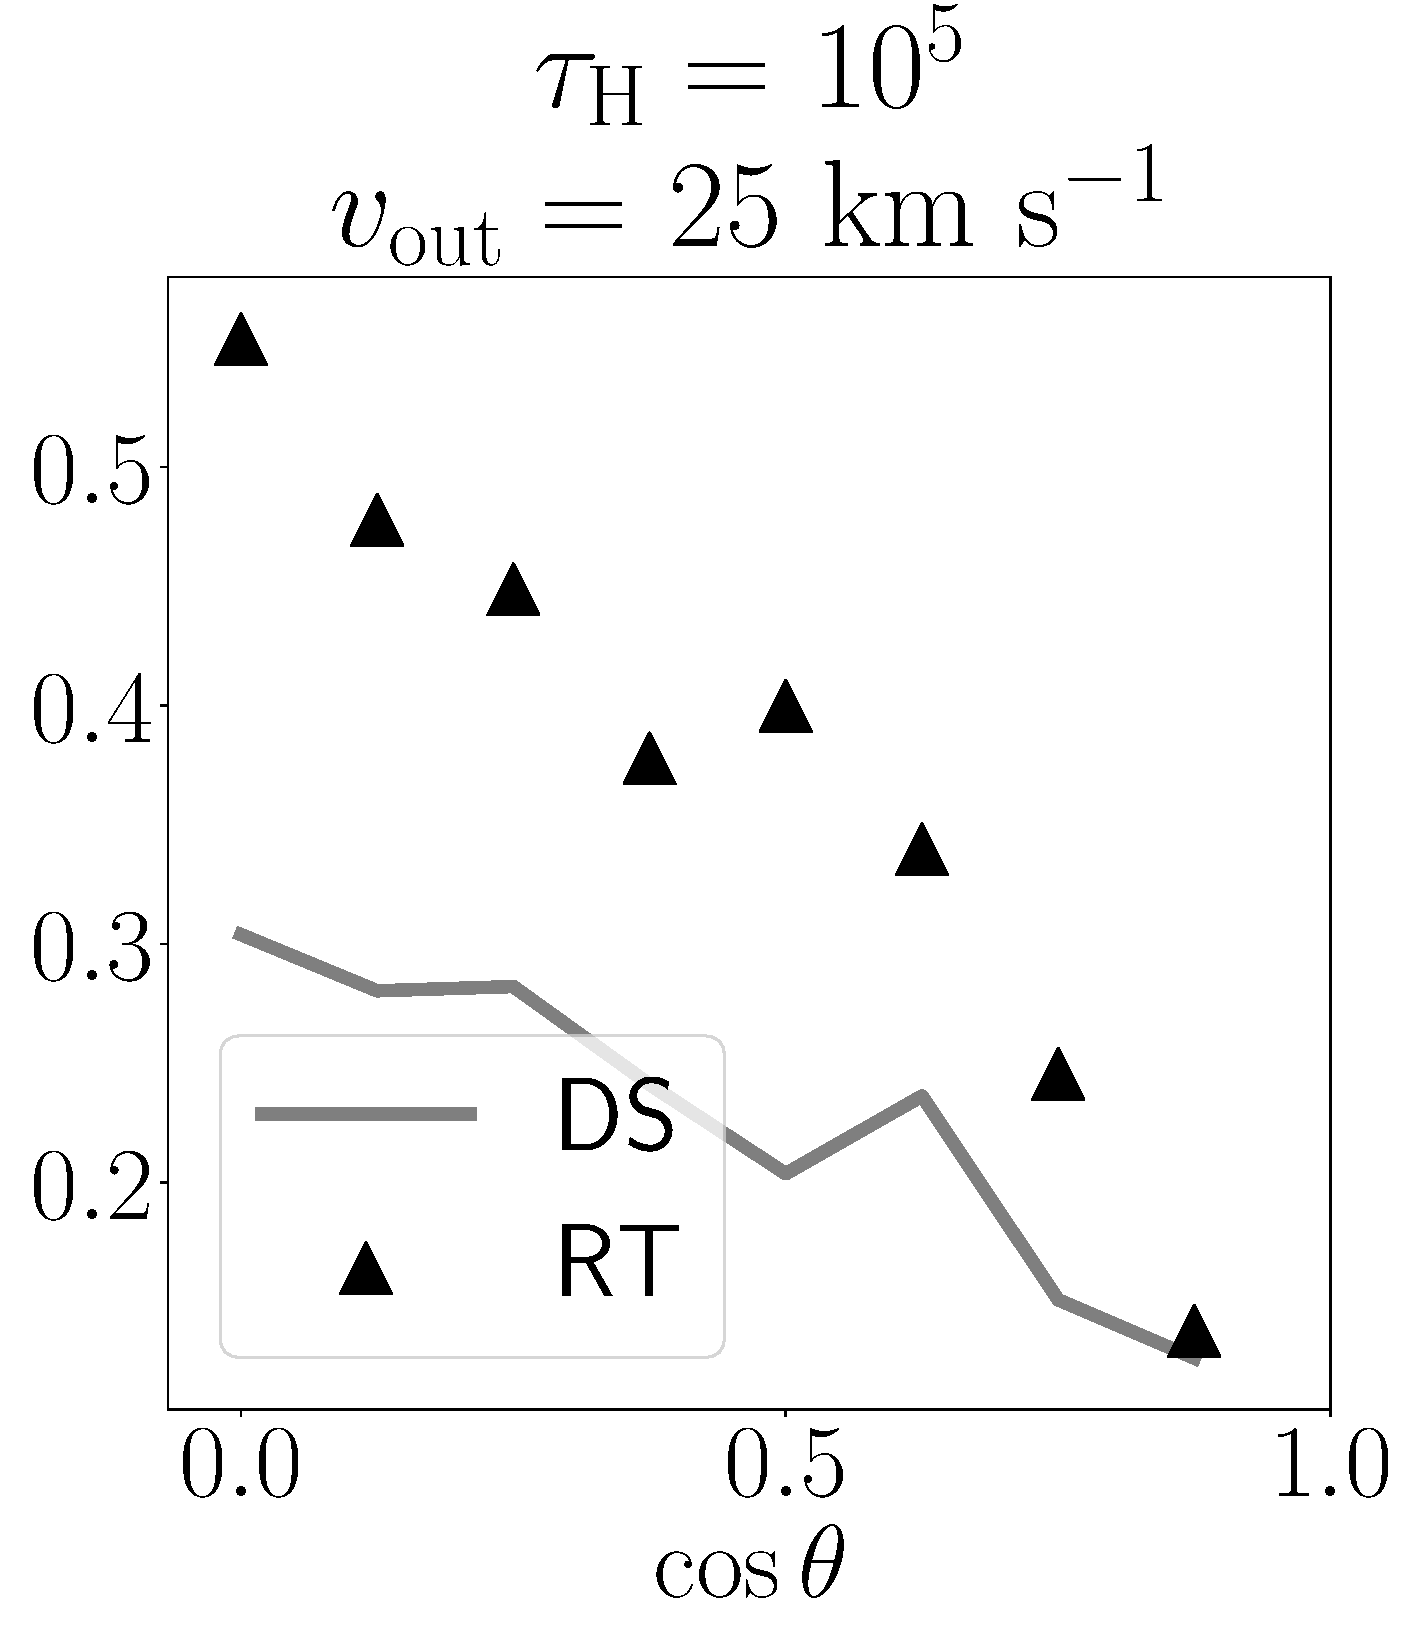
\includegraphics[height=0.28\textwidth]{./figures/results/line_characterization_vi_vout25_vrot100_logtau5}
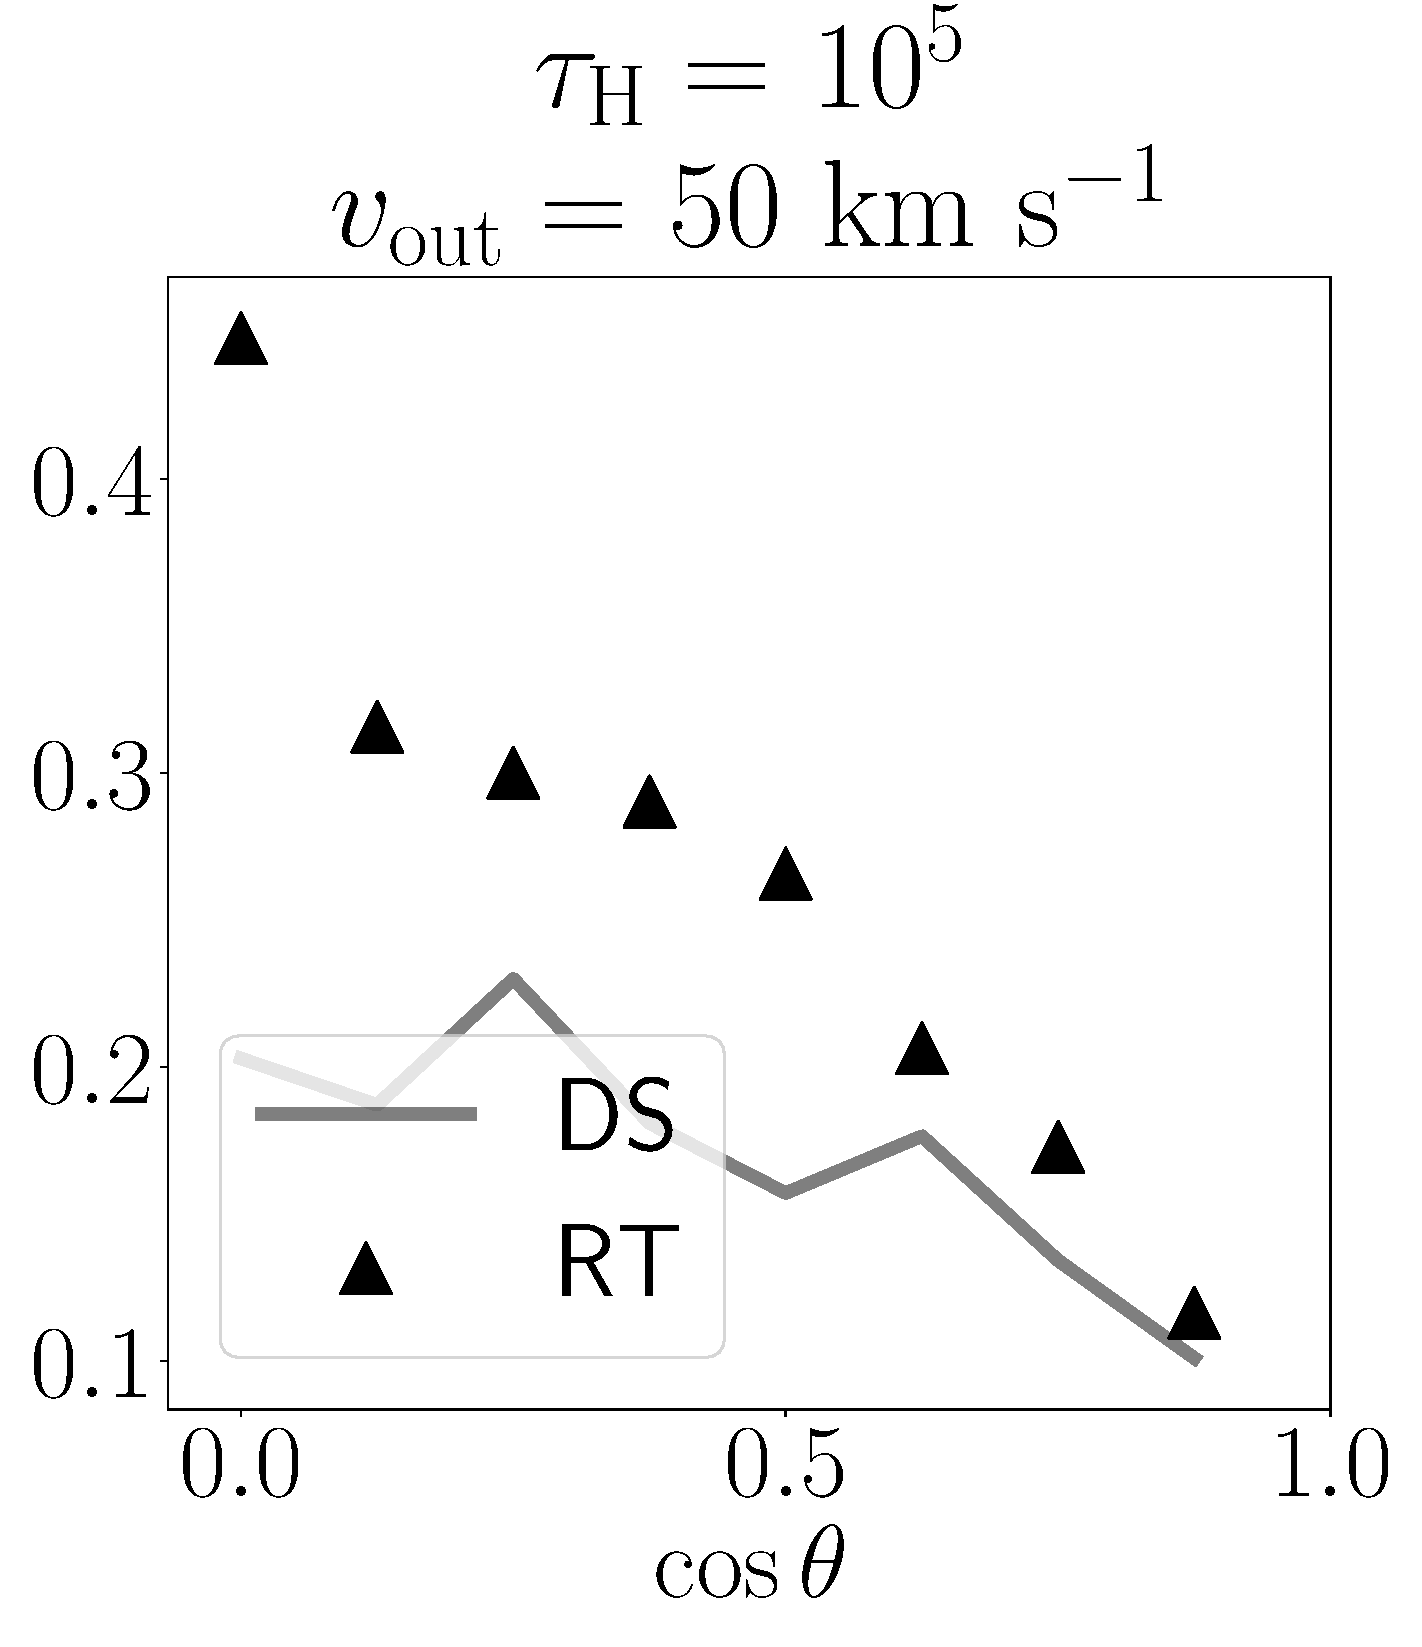
\includegraphics[height=0.28\textwidth]{./figures/results/line_characterization_vi_vout50_vrot100_logtau5}
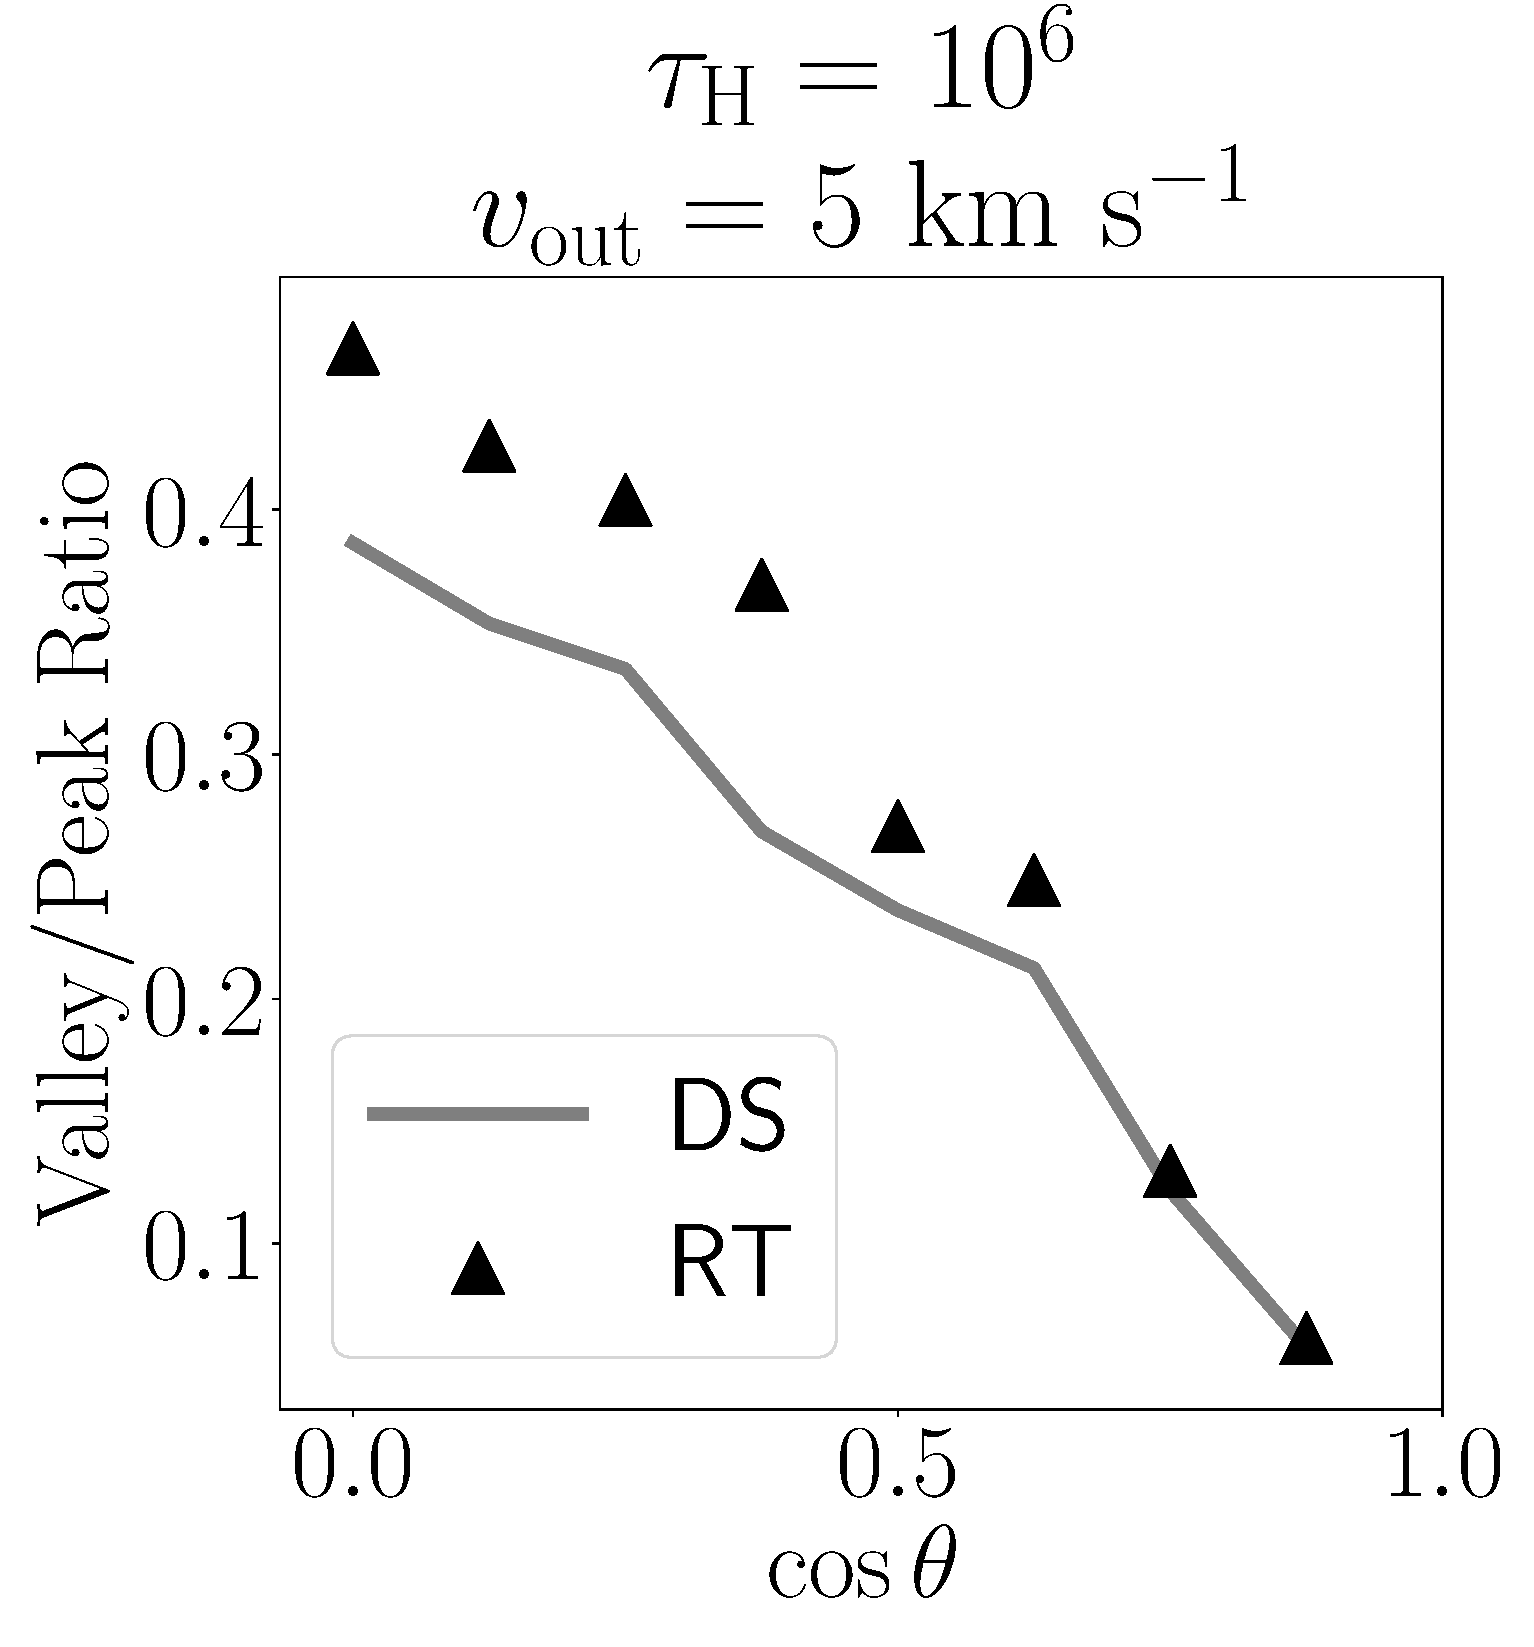
\includegraphics[height=0.28\textwidth]{./figures/results/line_characterization_vi_vout5_vrot100_logtau6}
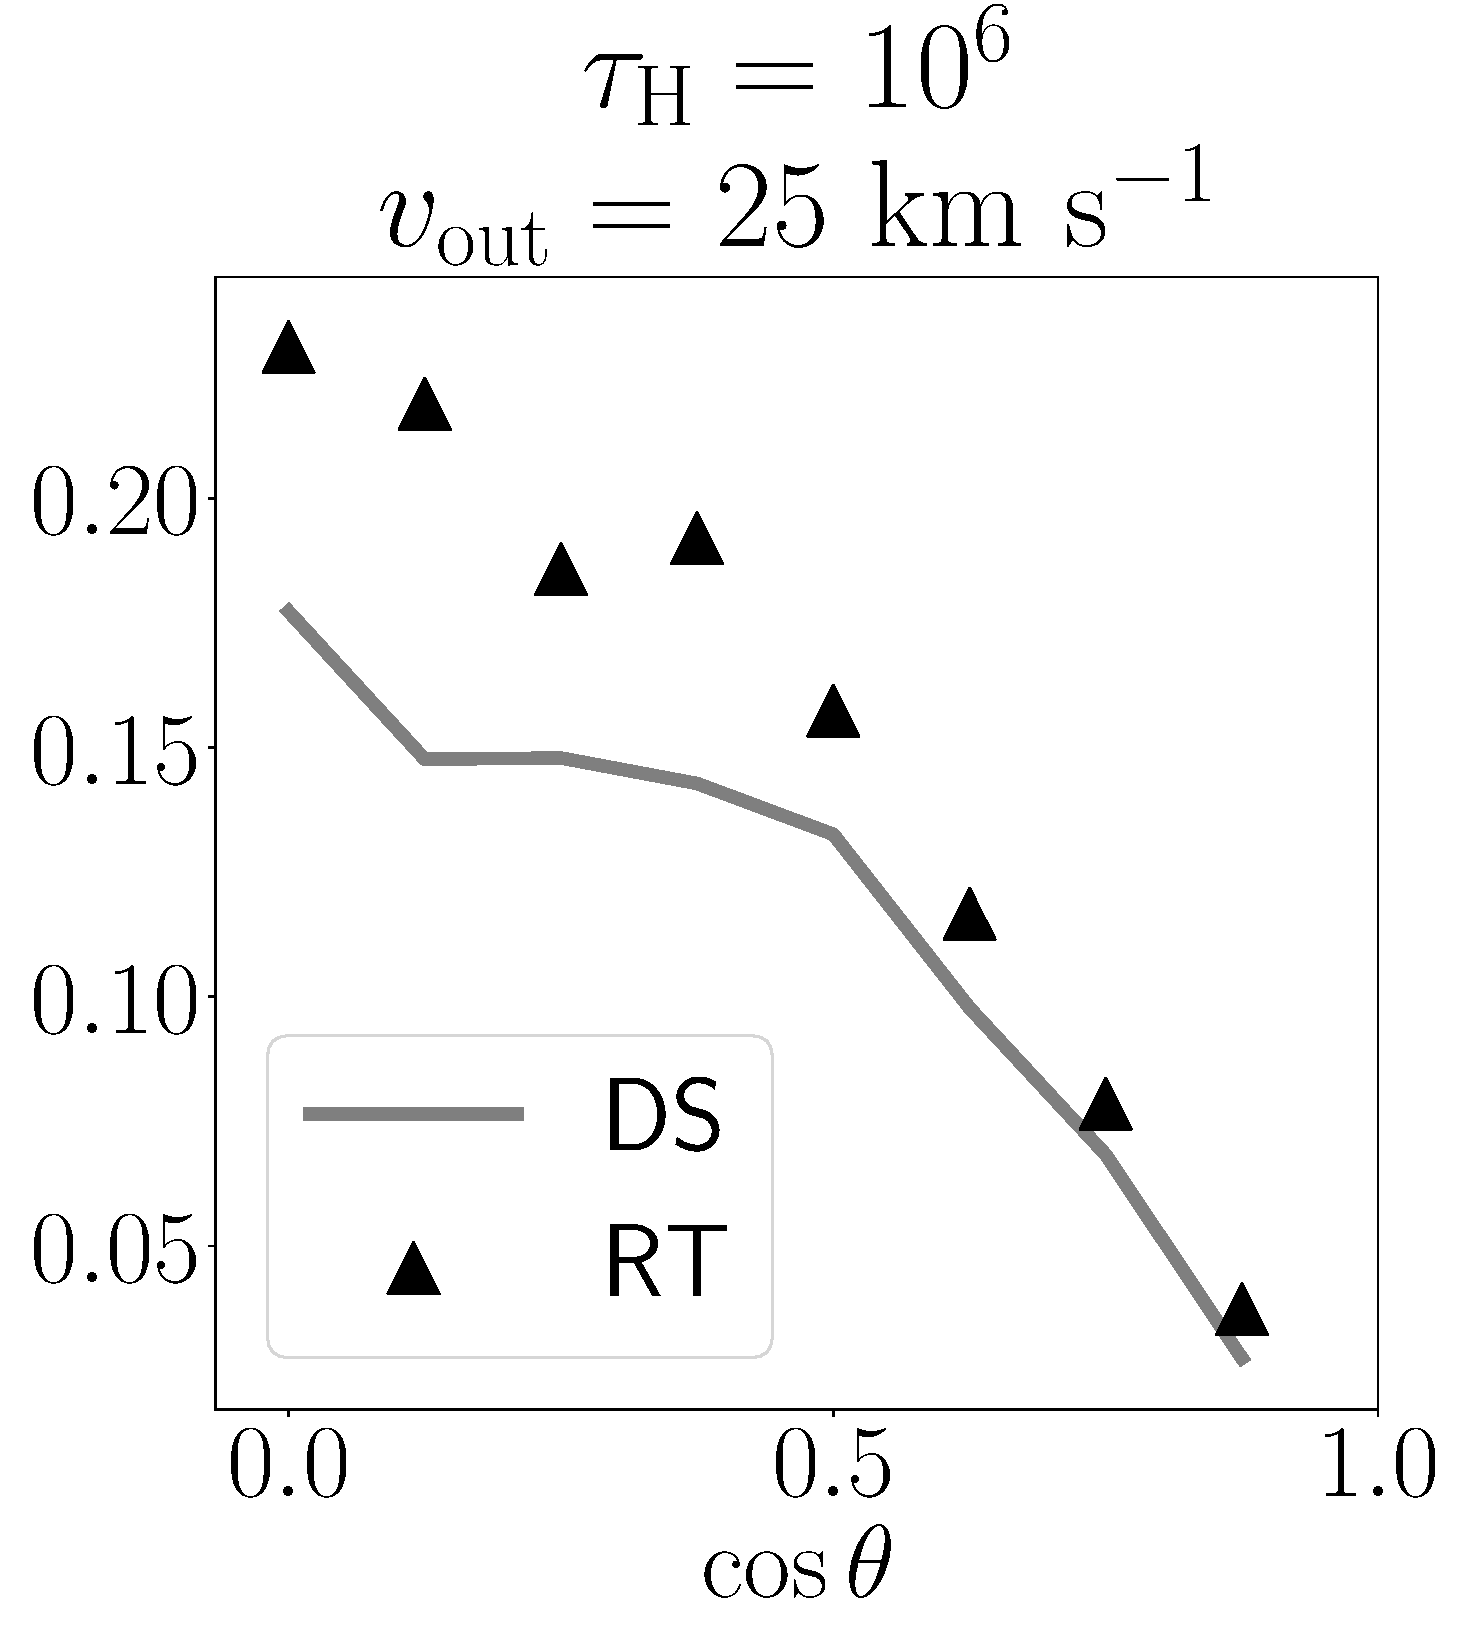
\includegraphics[height=0.28\textwidth]{./figures/results/line_characterization_vi_vout25_vrot100_logtau6}
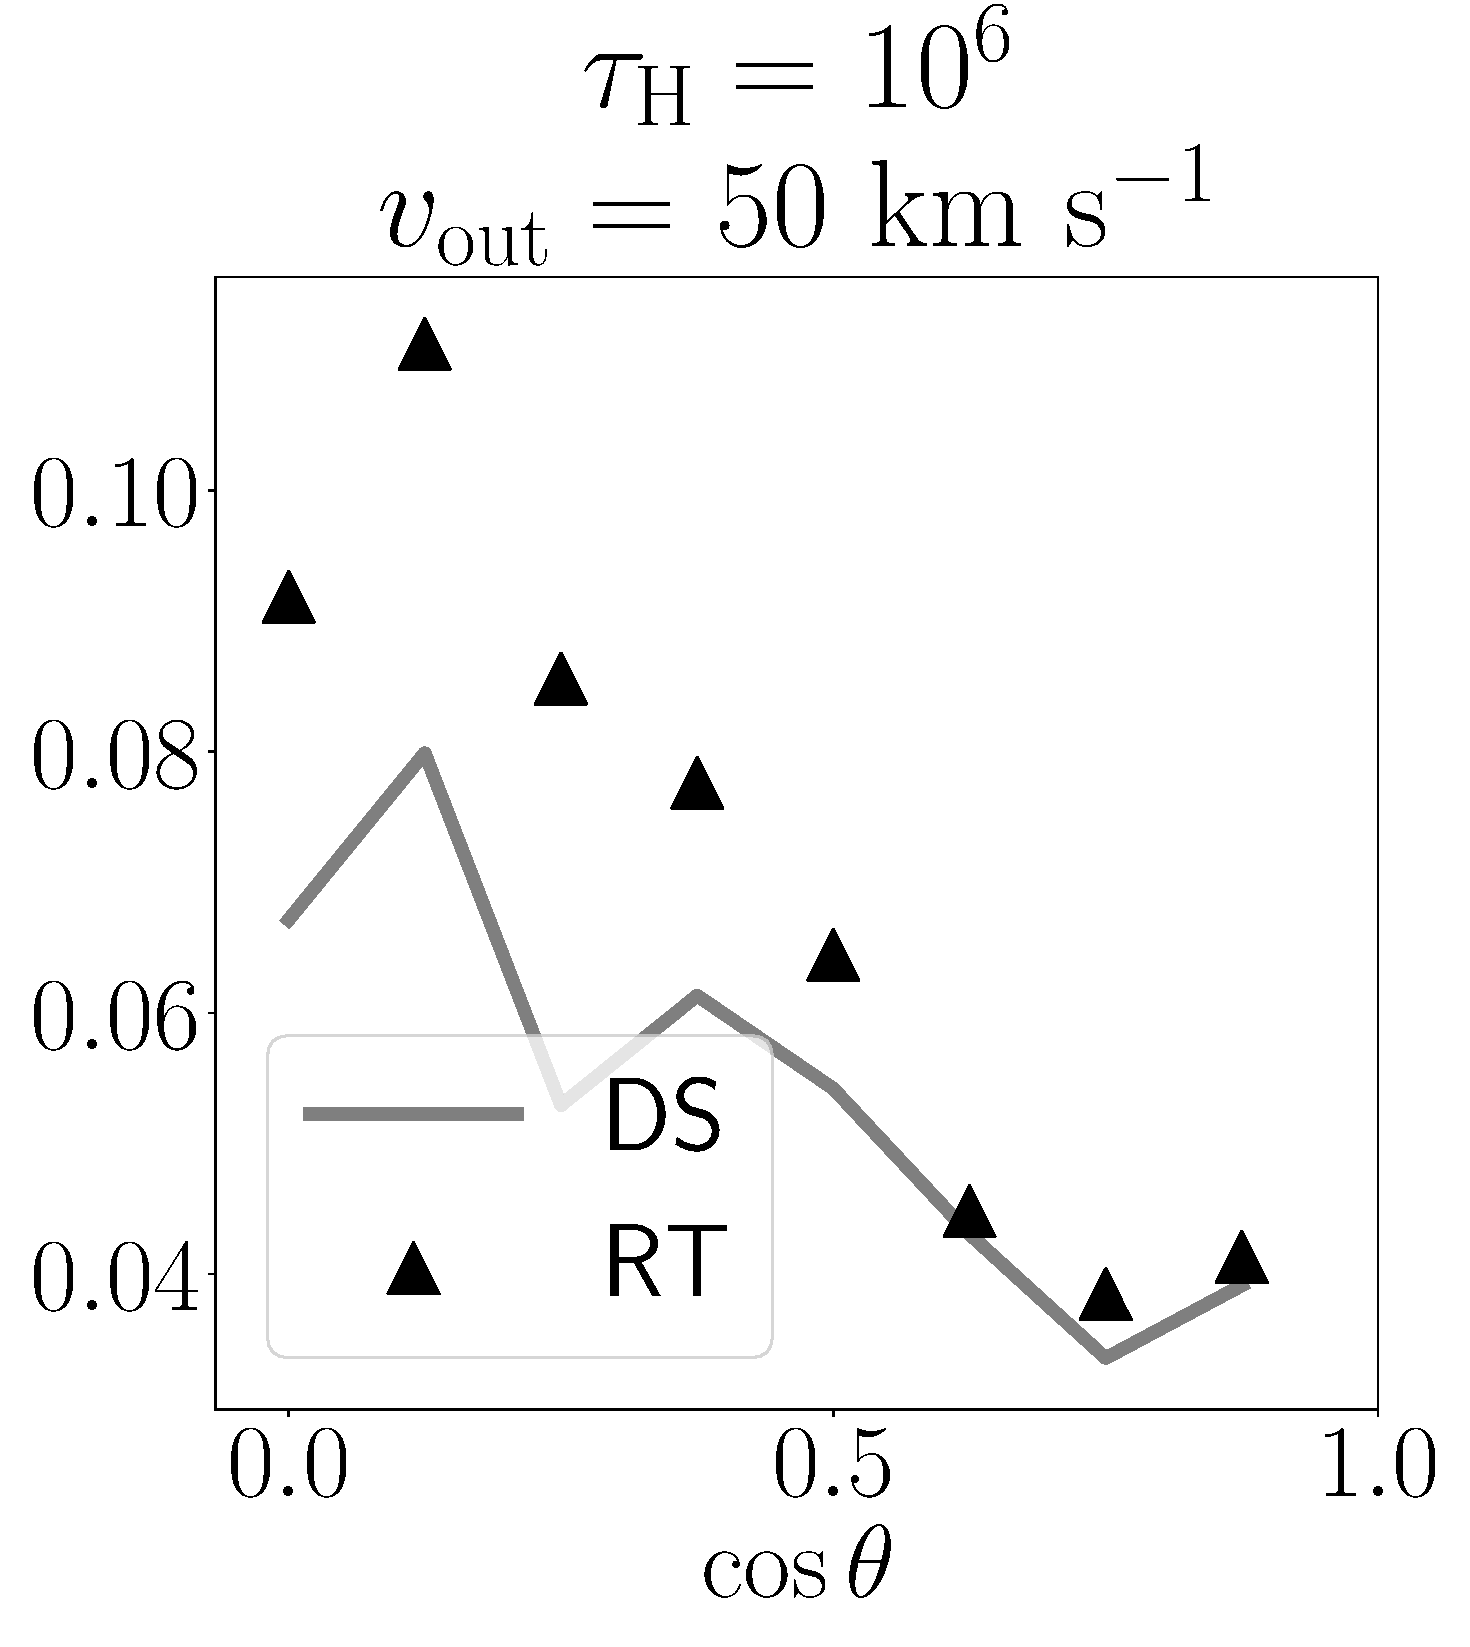
\includegraphics[height=0.28\textwidth]{./figures/results/line_characterization_vi_vout50_vrot100_logtau6}
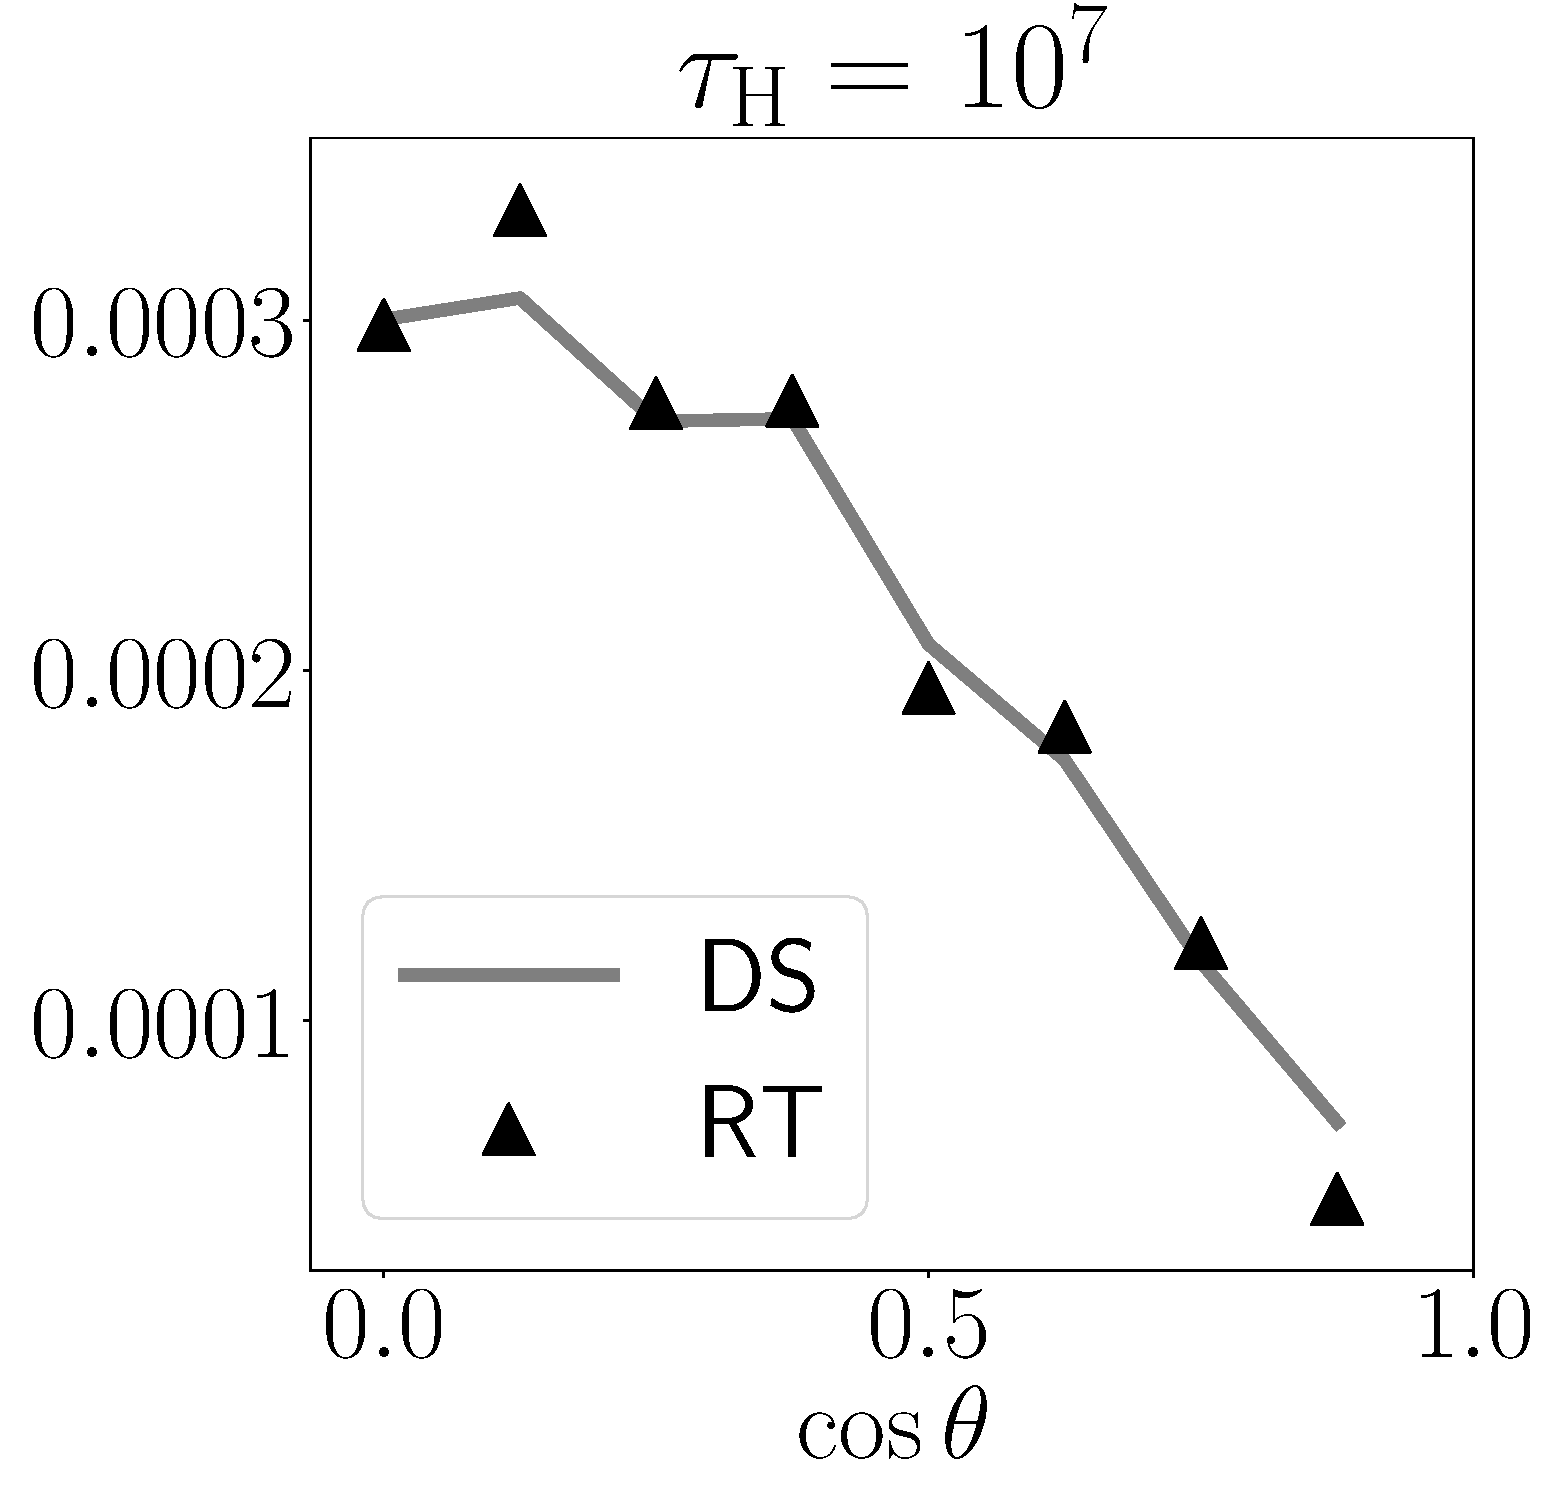
\includegraphics[height=0.28\textwidth]{./figures/results/line_characterization_vi_vout5_vrot100_logtau7}
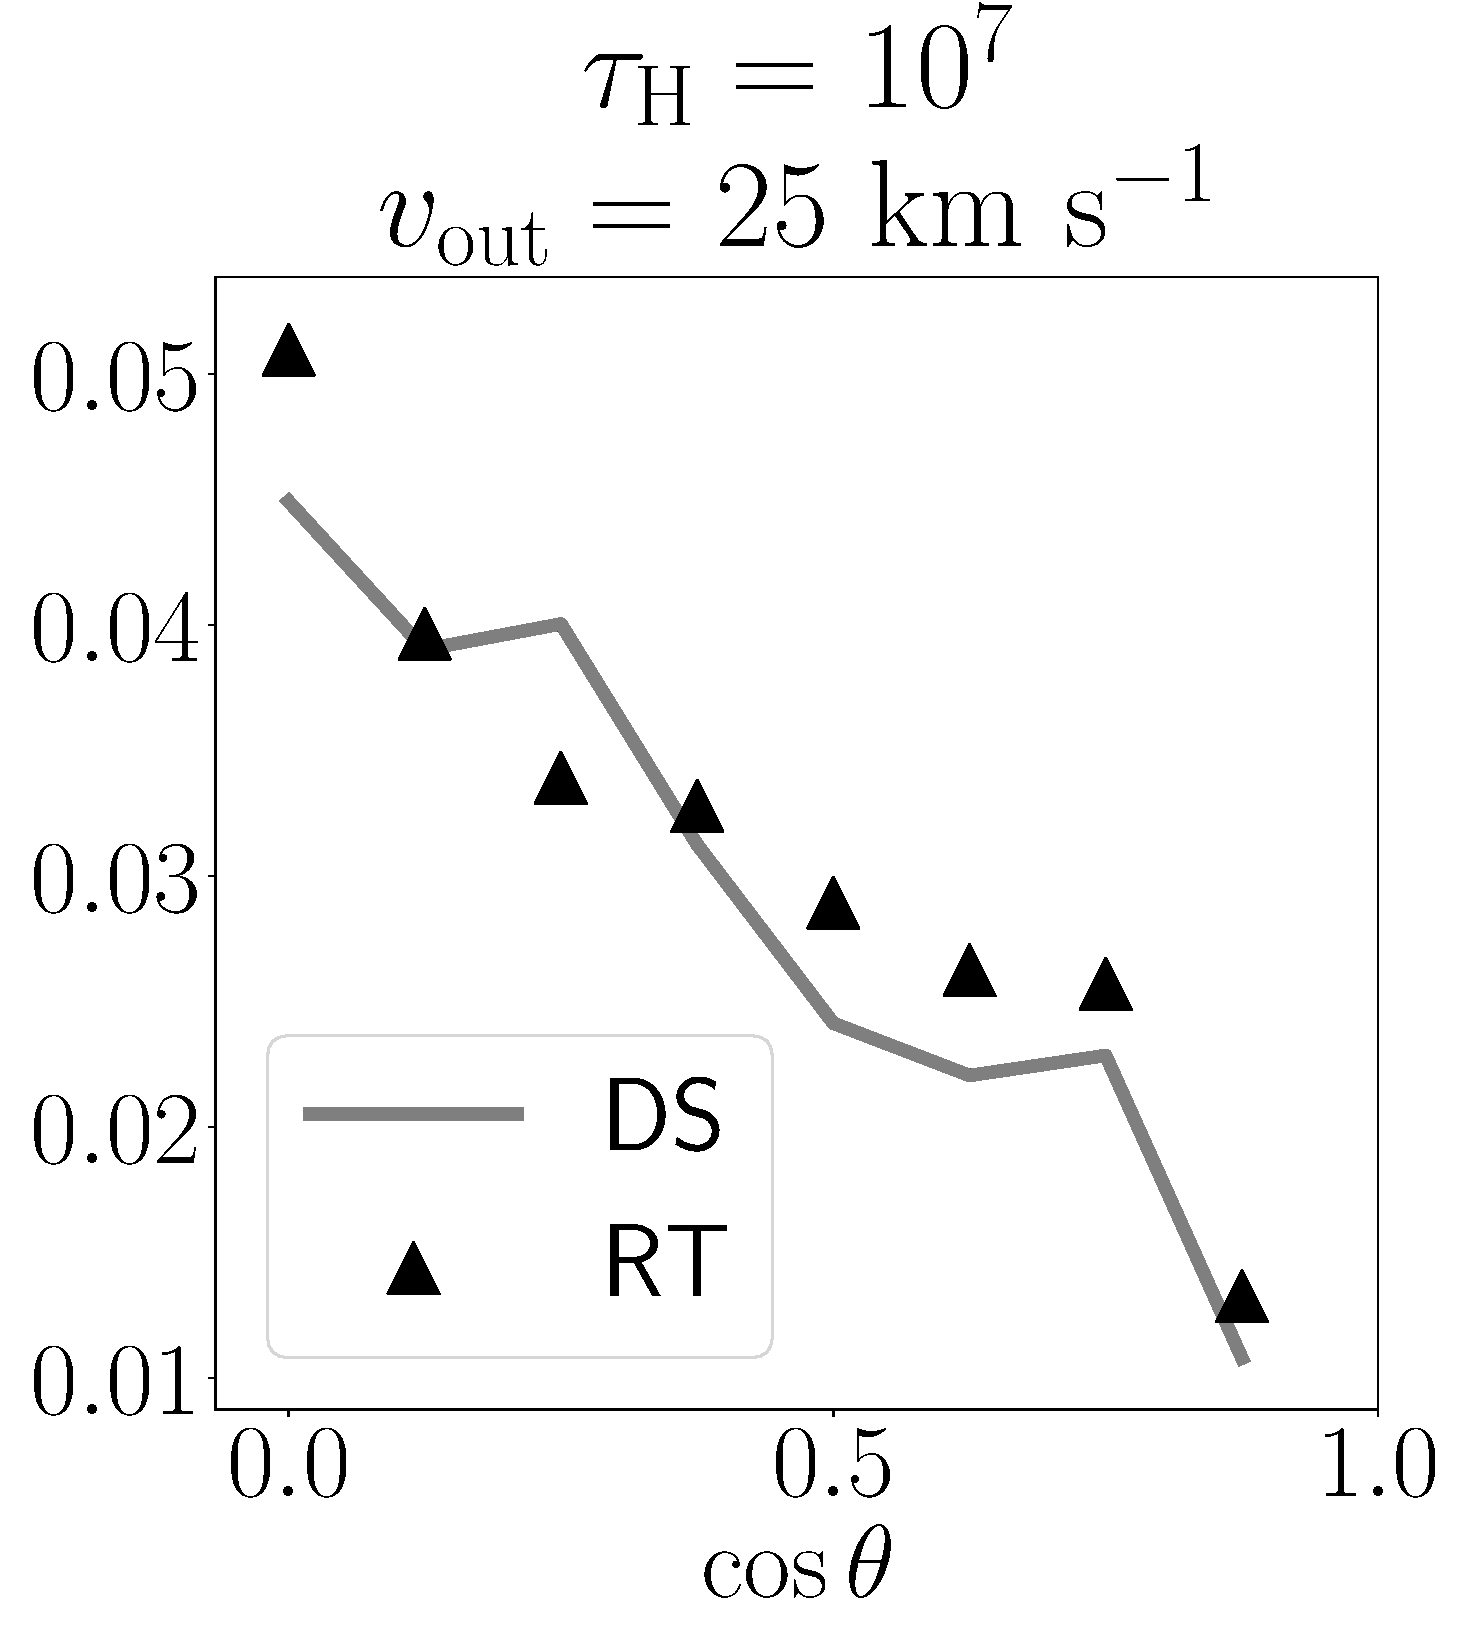
\includegraphics[height=0.28\textwidth]{./figures/results/line_characterization_vi_vout25_vrot100_logtau7}
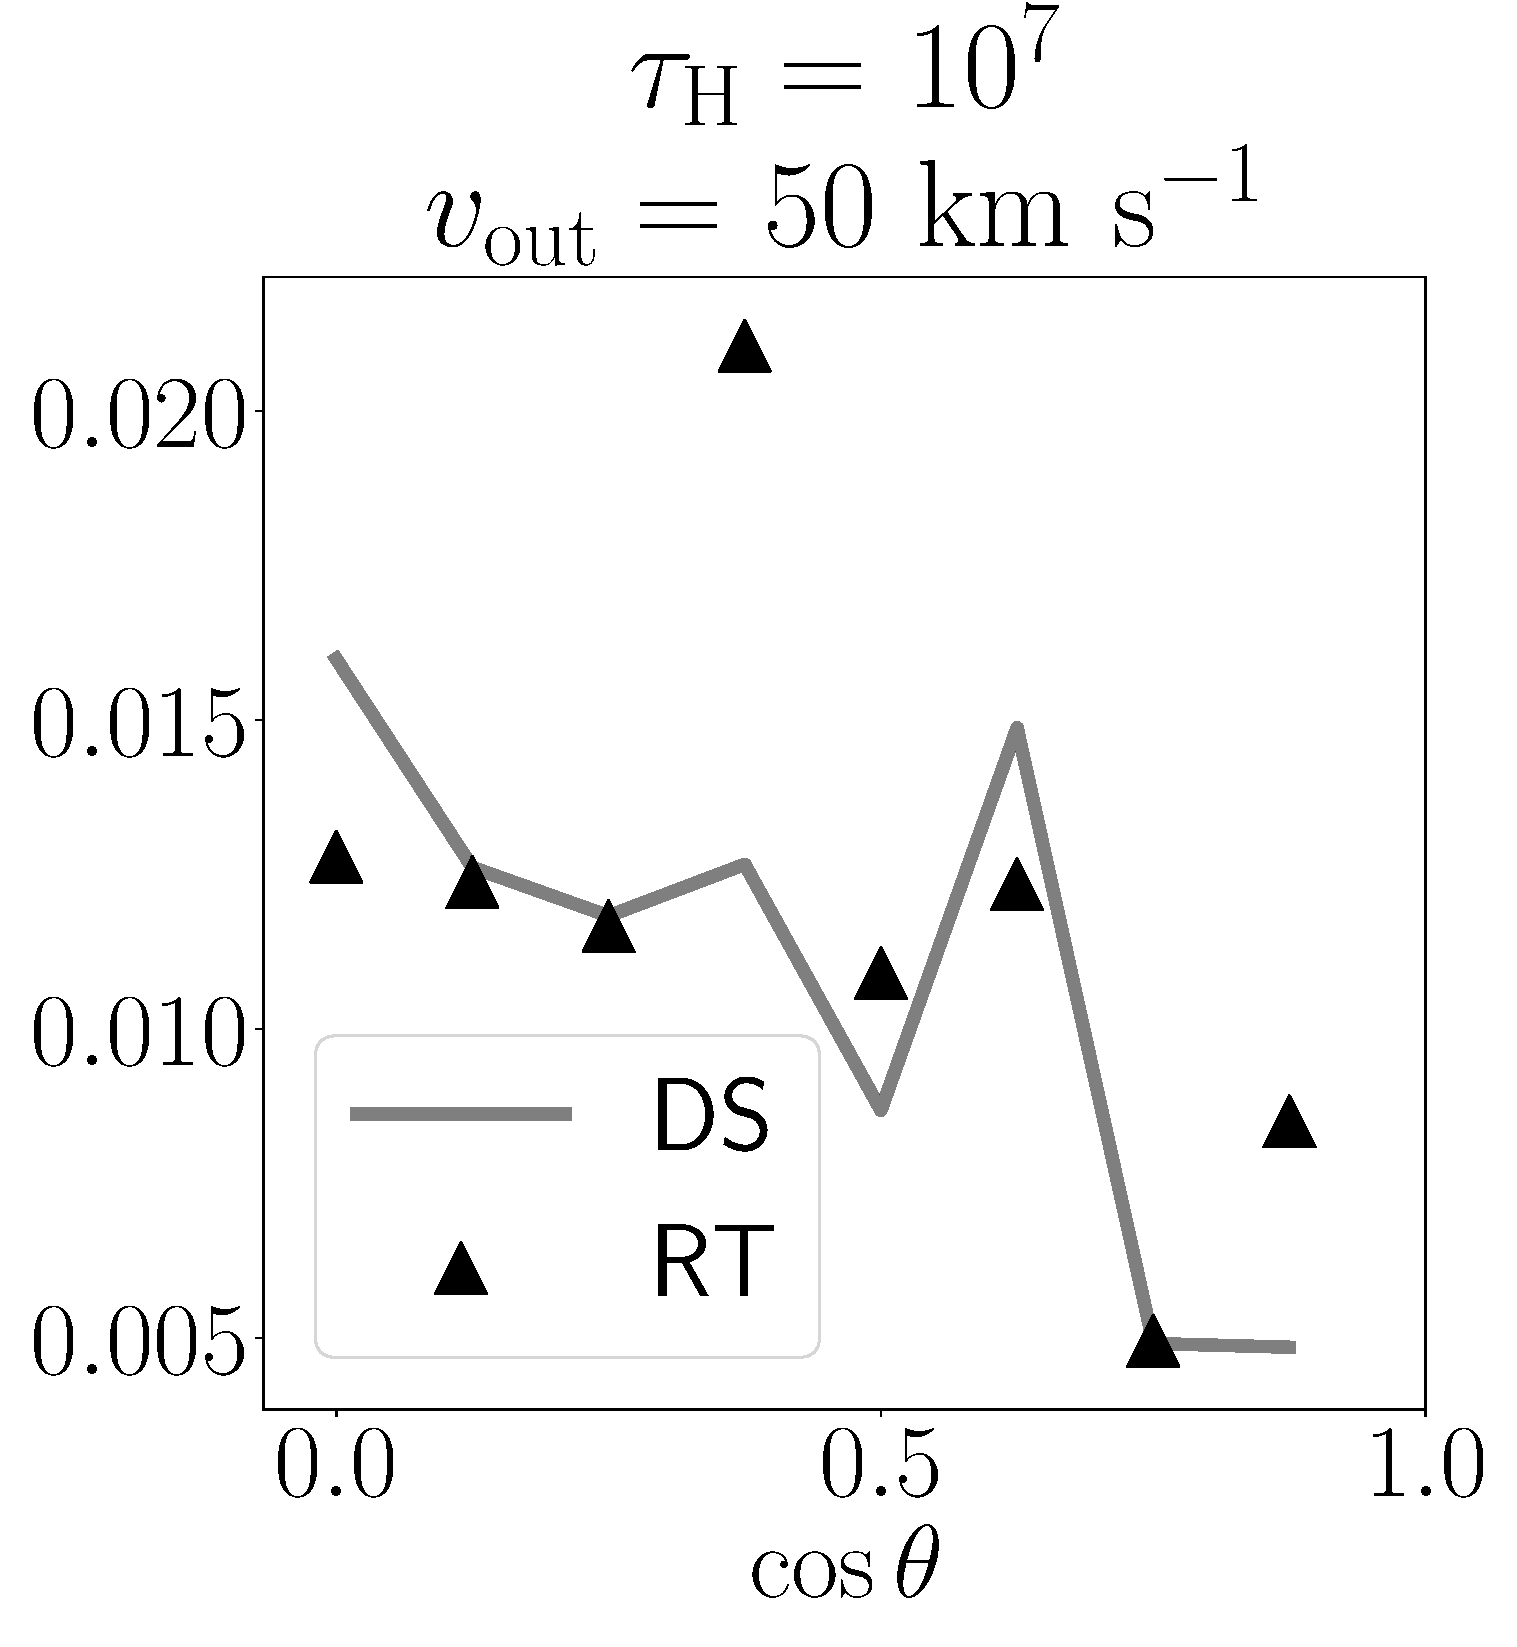
\includegraphics[height=0.28\textwidth]{./figures/results/line_characterization_vi_vout50_vrot100_logtau7}
\end{center}
\caption{\textbf{Valley Intensity:} We show for each \tauh the dependency that
		the viewing angle $\theta$ has on the line's the valley intensity. The larger
		$\cos{\theta}$ the lower is the valley intensity, so the higher $\theta$, the
		higher the valley intensity. Also, the higher \tauh, the better is the fit RT-DS.
		We fixed $\vrot=100$\kms.
		\label{fig:valley_intensity}}
\end{figure*}



\begin{figure}
  \begin{center}
    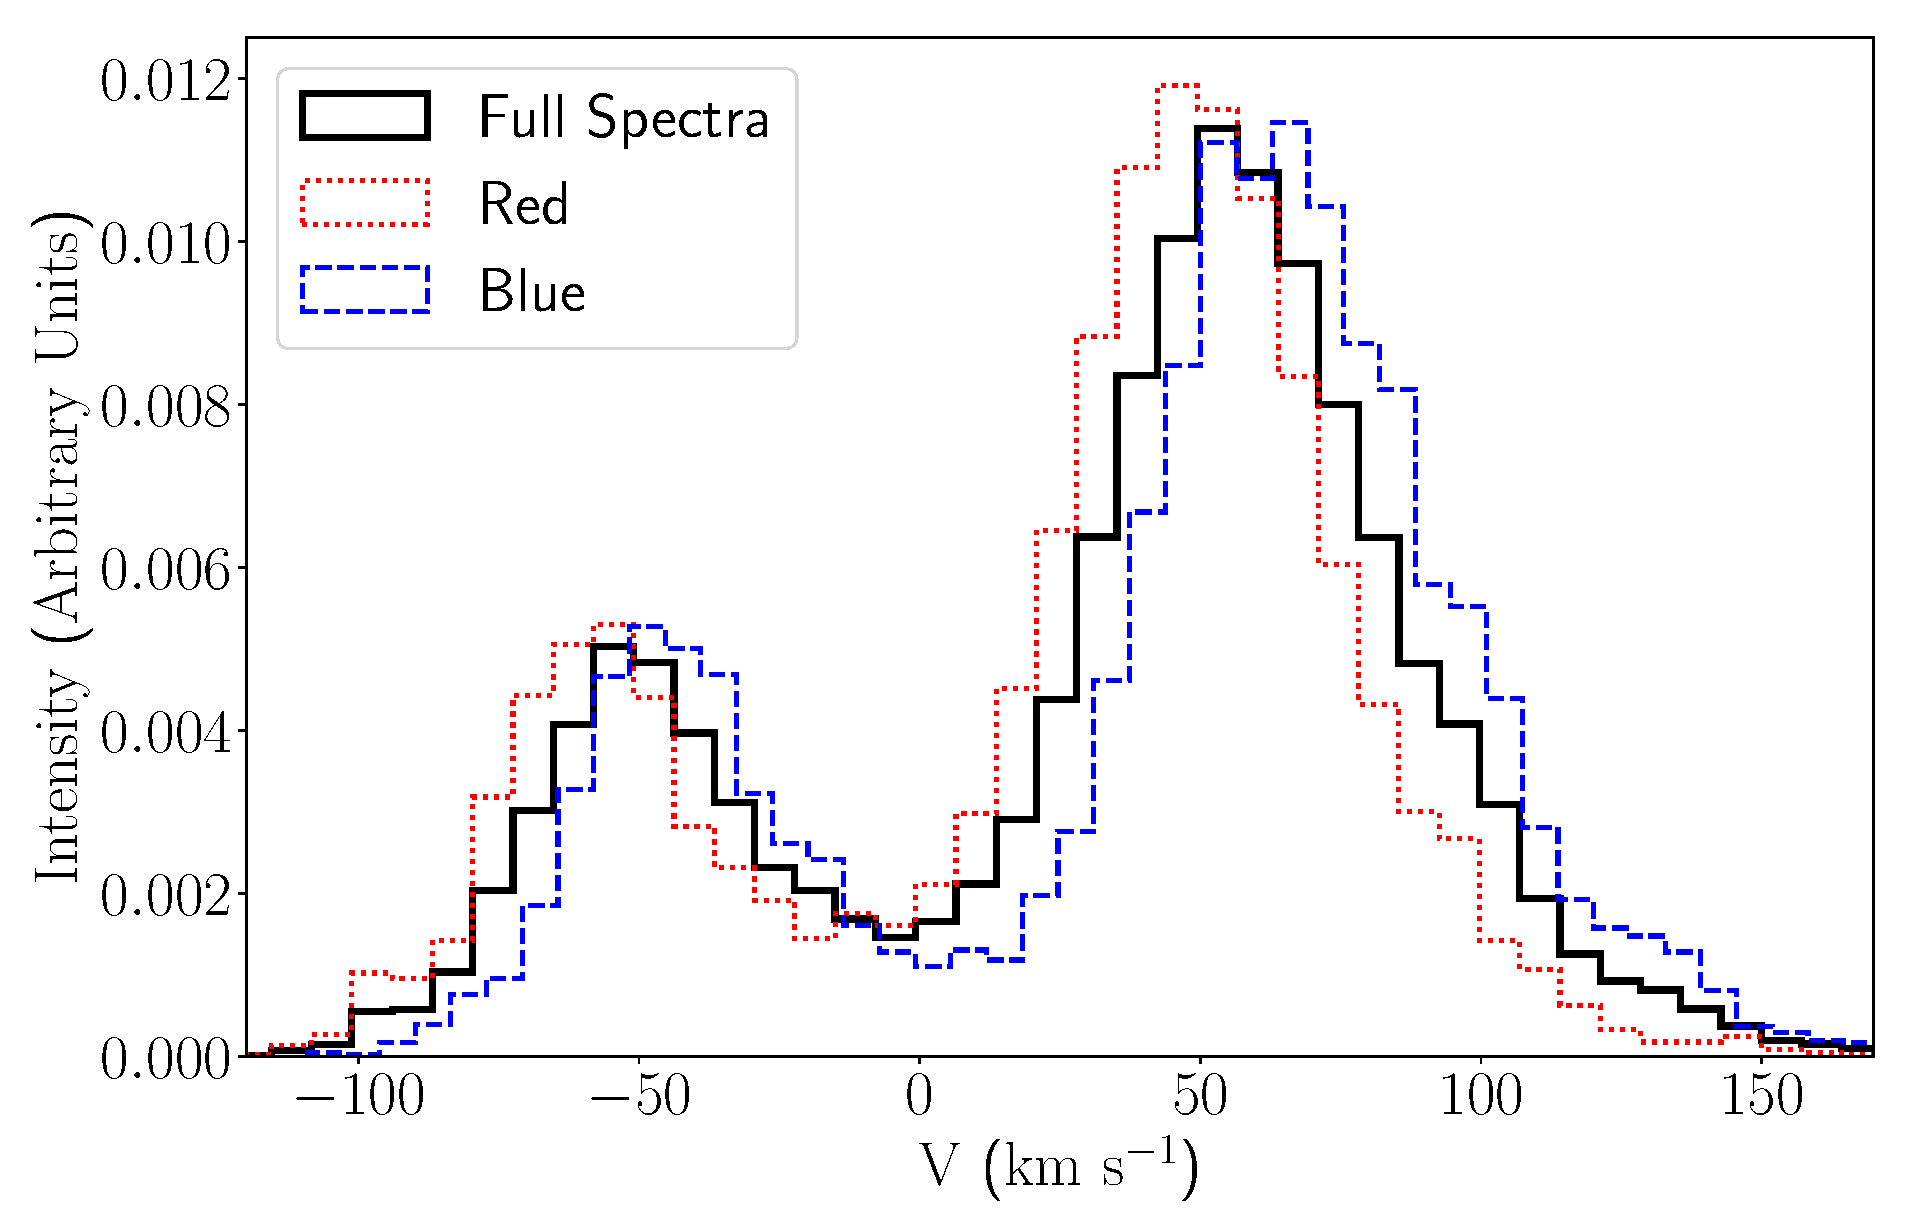
\includegraphics[width=0.48\textwidth]{./figures/discussion/doppler}
  \end{center}
  \caption{\textbf{Spectra from receeding/approaching sides of a toy
      model LAE.}  These results correspond to the RT simulation with
    $\vout=25$\kms, $\vrot=50$\kms, $\tauh=10^5$. 
    The spectra were computed for a viewing angle of
    $\theta=90^{\circ}$. This toy model illustrates to what extent spectra from
    opposite sides of a galaxy have an imprint of the rotational
    kinematics. 
    \label{fig:doppler}}
\end{figure}


\begin{figure}
  \begin{center}
    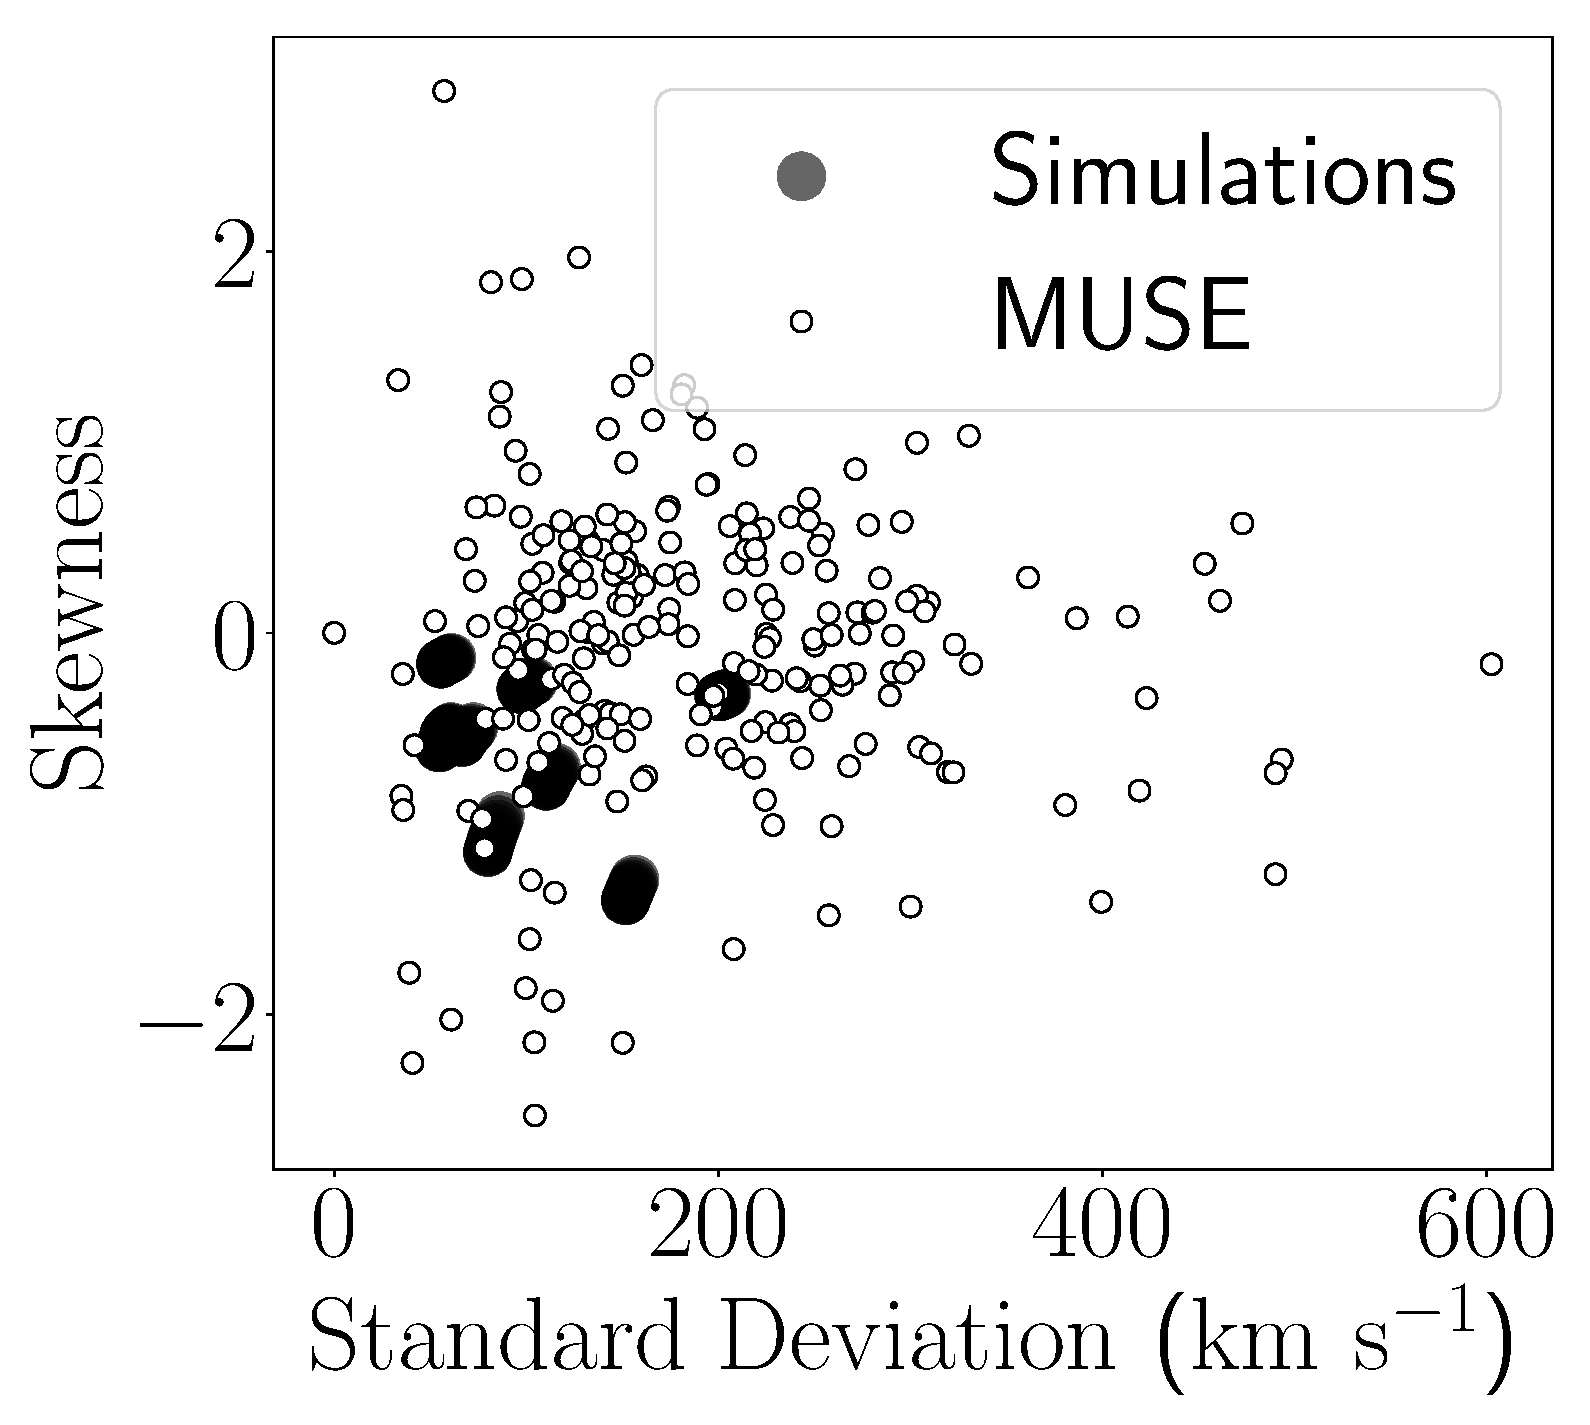
\includegraphics[width=0.48\textwidth]{./figures/results/muse_vs_simulations.pdf}
  \end{center}
  \caption{\textbf{Comparison between simulations and observations.}  
    \label{fig:muse}}
\end{figure}


\section{Theoretical Models}
\label{sec:theory}


The Monte Carlo code we use (CLARA)  follows the propagation of
individual photons through a neutral Hydrogen medium characterized by
its temperature, velocity field and global optical depth.
The code assumes an homogeneous density throughout the simulated
volume.
In the current implementation we neglect the influence of dust.
Our basic model is an spherical distribution of neutral hydrogen,
an approximation commonly used in the literature, as it explains a
wide variety of observational features
\citep{Ahn03,Verhamme06,Dijkstra06}. 


The velocity field we use captures both outflows and rotation.
Outflows are described by a Hubble-like radial velocity profile with
the velocity magnitude increasing linearly with the radial
coordinate; the outflows model is fully characterized by $v_{\rm out}$, the
velocity at the sphere's surface.
Rotation follows a solid body rotation profile, which is fully
characterized by $V_{\rm rot}$, the linear velocity at the sphere's surface.

The total velocity field corresponds to the superposition of rotation and
outflows.
The cartesian components take the following form:

\begin{equation}
	v_{x}=\frac{x}{R}V_{\rm out}-\frac{y}{R}V_{\rm rot} ,
	\label{eq:vx}
\end{equation}

\begin{equation}
	v_{y}=\frac{y}{R}V_{\rm out}+\frac{x}{R}V_{\rm rot} ,
	\label{eq:vy}
\end{equation}

\begin{equation}
	v_{z}=\frac{z}{R}V_{\rm out},
	\label{eq:vz}
\end{equation}
%
where $x$, $y$ and $z$ are the cartesian position coordinates with the
origin at the sphere's center, $R$ is the radius of the sphere and the
direction of the angular velocity vector corresponds to the $\hat{k}$
unit vector.

For each model setup we follow $10^5$ individual photons generated at
the center of the sphere at the \lya\ line's center as they propagate
through the volume and finally scape.
We store the final frequency and propagation direction for each photon
at its last scattering.

As input parameters we use \tauh$=\{10^5, 10^6, 10^7\}$,
\vout$=\{5,25,50\}\kms$ and \vrot$=\{0,50,100\}\kms$, for a total of
$27$ models with all the possible parameter combinations.
The range of values have some overlap with the expectations from a
galaxy with a total neutral hydrogen mass of $10^8$-$10^9$
$M_{\odot}$. 


\cite{Garavito14} presented an analytical model that
accounts for the effects of pure rotation on the
\lya\ line morphology. 
The basic assumption of their analytical model is that each
differential surface element on the sphere Doppler shifts the photons
that it emits.
In this paper we introduce this ansatz by post-processing the results
of the outflows simulations without rotation.
The frequency of each photon is Doppler shifted as follows

\begin{equation}
x' = x + \frac{\vec{V}_{\rm rot}\cdot\hat{k}}{v_{\rm th}}
\label{eq:shift_x}
\end{equation}
%
where $x'$ is the photon's new frequency, $x$ is the photon's
frequency after being procesed by the outflow, $v_{\rm rot}$ is the 
rotational velocity at the point of escape of the photon, $\hat{k}$ is
the photon's direction of propagation and $v_{\rm th}$ is the thermal
velocity of the sphere.

This allows us to produce new \lya spectra and compare them with the
full radiative transfer solution including both outflows and
rotation.

\section{Results}


\label{sec:results}

\subsection{Qualitative Trends}
\label{sec:qualitative}
Figure \ref{fig:doppler_shift} summarizes the most important trends.
The six panels correspond to $\tau=10^6$ and a viewing angle of
$\theta =90^{\circ}$, that is, perpendicular to the rotation axis of the
galaxy. 
In every panel the thin black line corresponds to the pure outflow
solution, i.e. without rotation. 
From top to bottom we see the effect of increasing the outflow
velocity, which is the expected increasing asymmetry towards the red
peak. 

The thick black line corresponds to the solution that includes both
outflows and rotation.
Comparing the left and right columns (lower versus higher rotational
velocity) we can see two immediate effects.
First, the line broadens and second, the intensity at the line's
center increases.

The thick gray line correspods to the pure outflow solution
with the Doppler boost added to model rotation's influence.
At $\tauh=10^6$ the Doppler boost does a good job at capturing the broad
morphological features introduced by rotation: the angle dependence,
the broadening and the intensity increase at the line's center.


In Figure \ref{fig:doppler_shift_theta_0} we show the same results as
in Figure \ref{fig:doppler_shift} but for a viewing angle of $\theta =
90^{\circ}$, that is parallel to the rotation axis. 
In this case we confirmethe result presented by \cite{Garavito14},
namely that pure rotation introduces a strong dependence with 
viewing angle, a trend that we find also holds for rotation mixed with
ouflows.   

The quality of the results from the Doppler boost improves for higher
\tauh values. 
In the Appendix we show the same plots as Figures
\ref{fig:doppler_shift} and \ref{fig:doppler_shift}, there it is
evident that for $\tauh=10^5$ the results are not as good as they are
for $\tauh=10^6$, and that for $\tauh=10^7$ the Doppler boos
provides a remarkable good approximation.

\subsection{Quantitative trends}
\label{sec:quantitative}


After finding the quantitative influence of the different parameters we
move onto a qualitative study.
To do this we summarize the line morphology by four different
characteristics: standard deviation (STD), skewness (SKW), bimodality
(BI) and valley/peak ration.
These quantities are defined by the following equations \citep{kokoska1999}.:

\begin{equation}
\label{eq:std}
\mathrm{STD} = \sqrt{m_2},
\end{equation}

\begin{equation}
\label{eq:skw}
\mathrm{SKW} = \frac{m_3}{m_2^{3/2}},
\end{equation}

\begin{equation}
\label{eq:bi}
\mathrm{BI} = \mathrm{KURTOSIS} - \mathrm{SKW}^2 = \frac{m_4}{m_2^{2}} - \frac{m_3^2}{m_2^{3}},
\end{equation}
%
where each $m_i$ is the i-th moment about the mean. 
The STD has velocity units and quantifies the line's width.
The SKW is adimensional and quantifies the peaks' asymmetry. 
In the case of a bimodal distribution, $SKW>0$ means that the blue
peak is taller and for $SWK<0$ the red peak is taller. 
The BI is adimensional and quantifies whether the line has 1 or 2
peaks: it is  always $\geq 1$ \citep{Pearson1929} and the 
to 1, the more bimodal is the line (i.e. has 2 similar peaks). 
We found by visual inspection of our spectra that BI$=2.5$ marks the
transition between two peaks (however imbalanced) and a dominang
single peak.


\subsubsection{Standard Deviation}
Figure \ref{fig:standard_deviation} summarizes the standard deviation
results for all our models.
Each panel shows the STD as a function of \vrot.
All panels were computed using a viewing angle of $\theta =
90^{\circ}$ (perpendicular to the rotation axis), which has the most
extreme ifluence from rotation.
 The black triangles
correspond to the full RT solution and the line to the DS
approximation.  
The optical depth increases from top to bottom and the outflow
velocity from left to right.
This quantitative plot confirms that the line width increases with
rotational velocity and optical depth.
These trends are expected; higher rotational velocities can be seen as
an addition of different Doppler shifts that smear out the line, while
a higher optical depth translates into a larger number of scatterings
that increase the probability of a photon to diffuse in frequency
resulting in a broader line.

The DS successfuly reproduces all trends with the optical depth,
rotational velocity and outflow velocity.
However, the DS consistently underestimates the STD. 
The difference between the RT and DS increases with the outflow
velocity and the rotational velocity, and decreases with increasing
optical depth.
In the range of parameter space explore, this difference has as an
upper bound of $\sim 7\%$, $3\%$ and $\sim 2\%$ for
 $\tauh=10^5$, $10^6$ and $10^7$, respectively. 

\subsubsection{Skewness}

Figure \ref{fig:skewness} presents the skwewness results for all the
models together with the DS comparison following the same layout as
Figure \ref{fig:standard_deviation}.
In all cases the skewness is negative showing that all the lines
are unbalanced towards the red side of the spectrum.
Skewness increases with rotational velocity and decreases with
optical depth; rotation tries to smoothes the line diminishing the
asymetries while a higher optical depth reinforces the line asymetries.
The skewness does not have a monotonous trend with outflow velocity because
there is a transition between double and single peak line; for low
outflow velocities the skewness signals the balance between the two
existing peaks while for high outflow velocities it quantifies the
asymmetry of the already dominant read peak.

The DS reproduces the main trends, again with an underestimation that
decreases at higher optical depths and increases with larger values of
the rotational velocity and outflow velocity.
In this case the differences between RT and DS have an upper bound of
$85\%$, $35\%$ and $5\%$ 
for  $\tauh=10^5$, $10^6$ and $10^7$,
respectively.  


\subsubsection{Bimodality}

Figure \ref{fig:bimodality} shows the results for the bimodality using
the same layout as in the two previous Figures.
Following the reasoning about the skewness, we observe that
increasing the outflow velocity increases the value of bimodality,
that is, it transitions to a more pronounced single peak. 
The trend as a function of the rotational velocity and the optical
depth are not monotonous.
When the outflow velocity is low (\vout$<50\ \kms$), an increasing
rotational velocity smears the two asymmetrical peaks pushing the line
morphology towards a single peaks, making the bimodality statistics
increase. 
On other situations (\vout$=50\ \kms$ and \tauh$\geq 10^6$) higher
rotational velocities the bimodality statistics decreases, which means
that it manages to slightly enlarge the already dominant red peak.

The DS reproduces the main trends while underestimating the bimodality
statistics. 
As expected from the previous results the difference betwen RT and DS
decreases at higher optical depths and increases with increasing
values of the rotational and outflow velocities.
In this case the differences have an upper bound of $4\%$, $2\%$ and
$1\%$ for  $\tauh=10^5$, $10^6$ and $10^7$, respectively.  

\subsubsection{Intensity at line's center}

In Figure \ref{fig:valley_intensity} we quantify how the intensity at
the line's center (i.e. the valley) changes with the viewing angle,
the outflow velocity and the optical depth.
These results correspond to a fixed rotational velocity of
\vrot$=100\ \kms$.
The triangles correspond to the RT simulations and the line represents
the DS results. 
The valley intensity is expresed as a fraction of the maximum peak
intensty in the line, as such the valley/peak ratio is always less
than one. 
In every panel we see that the valley/peak ratio decreases as the
observer moves from a line  of sight perpendicular to the rotation
axis onto a parallel line of sight. 
This is a clear demonstration of the viewing angle dependency
introduced by rotation.

The valley/peak ratio at $\cos\theta=1$ matches results
without rotation, this shows that for increasing rotational velocity
the valley/peak ratio increases.
In turn, for increasing optical depth or outflowing velocity this
ratio decreases.
Once again, the DS results correctly follow the trends for the full RT
simulations.  
This time the differences have an upper bound of $55\%$, $2\%$ and
$1\%$ for  $\tauh=10^5$, $10^6$ and $10^7$, respectively.  






\section{Discussion}
\label{sec:discussion}


\subsection{Theoretical Insights}

A first approach to an analytical expression that returns the \lya spectrum
from a rotating galaxy is presented by \cite{Garavito14}.
This derivation is based on the assumption that the distribution of
photons' propagation directions at the edge of the galaxy is
anisotropic and depends of \tauh only. 
So this approximation becomes more accurate with higher optical depth
and it is also the reason why the Doppler Shift technique to induce
rotational effects to an outflow \lya spectrum works. 


\subsection{Links to observations}

There are at least three inmmediate ways the work we have presented
here can be useful to observational efforts.


\subsubsection{\lya continuum leakage or rotation?}

Another application of this new model to the current interpretation of \lya
spectra, is that the central ($V=0$) emission of the spectra seen in the
\lya line, is a consequence of the viewing angle of the galaxy and can be
controlled by it. 
Several authors have suggested that this central emission is caused by
radiation that escapes the galaxy without scattering. 
Rotation is an alternative that solves this issue. 

We note that the relative intensity of the two peaks in the outflowing
spectra is not modified by rotation, that asymmetry is solely
controled by the outflow velocity.
This means that results that have already derive a typical outflowing
velocity as to match the observational constraints do not have to be
completely revised. 
Only an additional exploration of rotational velocities and viewing
angles need to be explored.


\subsubsection{\lya Kinematic Maps}

Current observational facilities have the capability of spatially
resolving the extent of a LAE.
For instance \cite{Prescott14} presented observational results of a
Doppler shift when taking spectra at two oposite sides of a large
($\approx 80$kpc) LAE.

In Figure \ref{fig:doppler} we present a toy model (\vrot$=50\ \kms$,
\vout$=25\ \kms$ and \tauh$=10^5$) for the spectrum of
a LAE taken from to different sides of the galaxy. 
As the LAE is rotating, one side is being redshifted while the other
is blueshifted. 
We see that the full spectrum is a weighted line, in solid black,
that is found between these two.
We notice that the distance between the maxima of the blue and red
spectra is not twice the rotational velocity as it could be naively
expected.

Although it is a good approximation to think the rotating spectra by a
sum of Doppler shifts, the peak of the spectra is also weighted by the
amount of mass with a given velocity. 
In this toy model the distance between the peaks of the
receeding/approaching spectra is close to $\sim 20\ \kms$, which is
less than half of the naively expected value of $2\vrot=100\ \kms$,
due to the fact that only a small fraction of the photons are emitted
at the extreme of the galaxy having the maximum rotational velocity of
$50\ \kms$. 


New spectrographs like MUSE should help obtain kinematic information
from LAEs to build velocity maps in \lya. 
This could be a natural extension of the work reported by
\cite{Herenz2016} on the velocity maps of several LARS (Lyman Alpha
Reference Sample) galaxies.  
The interpretation of such data should take into account the insights
and trends we have presented in this paper.

\subsubsection{Comparison against the MUSE-Wide Survey}

In order to give the reader a feeling of the ranges of observational
data that could be explained by the models presented here, 
we perform a comparison against observational data from the MUSE-Wide
Survey (MWS) \citep{2017A&A...606A..12H}.   

MWS provides public access to 831 spectra out of which 237 contain a
detected \lya line as dominant. 
The public dataset reports as the redshift of the galaxy the position
of the dominant peak.
We use this redshift to convert the spectra to a rest-frame and compute
the standard deviation and skewness statitstics. 
Given the uncertainty on the galaxy redshift we do not compute the
valley/peak ratio. 
We do not try to perform a full fit to all the spectra
\citep[e.g.][]{2017A&A...608A.139G} and wish only to
know whether the region of parameter space explored in our RT
simulations shows any crossing with the results from the MWS or
shows any sign of atypical features.
 
Figure \ref{fig:muse} shows the results of this experiment. 
The small white circles correspond to the 217 \lya emitters in the MWS
observations; the large black circles to the results of the
simulations presented in this paper. 
This shows that the systems modeled in this paper actually present an
overlap with statistics derived from observations. 
The region with standard deviation $>200$\kms could also be explained
by systems with larger optical depths than we have used here. 
However, the systems with a positive skewness, that is a line
unbalanced towards the blue could be the sign of inflowing
kinematics. 

\section{Conclusions}
\label{sec:conclusions}

In this paper we explore, for the first time in the literature,
the results of a model for the emergent \lya\ line from rotating outflows.
The main results for the model are computed from a Monte-Carlo
radiative transfer simulation and confronted with a simple
semi-analytic ansatz that adds the effects of rotation onto results of
pure outflow kinematics. 

To address the first questionswe posed in the introduction (What is then
the expected imprint of rotation on a resonant emission line such as
the \lya line?)

We can saythat the main effects of rotation on the \lya\ line morphology are:

\begin{itemize}
  \item Inducing a dependency on the viewing angle.
  \item Broadening the line.
  \item Increasing the intensity at the line's center.
\end{itemize}

We find that these effects can be quantitatively explained by a
Doppler shift computed as product of quantities at the surface of last
scattering, namely  $\vec{v}_{\rm rot}\cdot \hat{k}$,  where
$\vec{v}_{\rm rot}$ is the velocity due to rotation and $\hat{k}$ is
the direction of the photon's propagation.  
These conclusions, specially the confirmation of the Doppler Boost as
a good approximation to model solid body rotation, strenghten the
semi-analytic model reported by \cite{Garavito14} when they modeled
the effect of pure rotation on \lya\ spectra. 


Addressing the second question we posed in the introduction (To what
extent is possible to constrain rotational kinematics from the \lya
emission line?)  we can say that as an application to observational data our results suggest that
rotation should also be considered as an explanation of the
non-vanishing \lya intensity at the line's center.

A more straightfoward approach is takes into account how the
\lya spectra from two different sides of a galaxy can detect
approaching/receeding gas motions.
In that case one has to be careful and take into account that the
peaks of these two spectra is smaller than the expected value of
$2\times\vrot$ due to the differente weights at the surface of the
emitting regions.   

We also use data from MUSE to demonstrate to what extent the
outputs of the RT results presented here can be expected to match
hundreds of observed \lya spectra, but a full constraint of rotation
properties certainly require a full Markov Chain Monte Carlo
exploration of parameter space.

Our work confirms that rotation produces features in the \lya line
strong enough that can be expected to be detected in observations and
that should be taken into account into \lya modelling; the Doppler
Boost offers an easy-to-implement approximation to explore such
influence into already existing RT simulations and provide stronger
footing to the interpretation of \lya kinematics maps
\citep[e.g][]{2018MNRAS.473.3907A}. 

\bibliographystyle{mnras}
\bibliography{references}


\newpage
\appendix

\section{Additional figures}
\label{sec:appendix}


\begin{figure}
  \begin{center}
    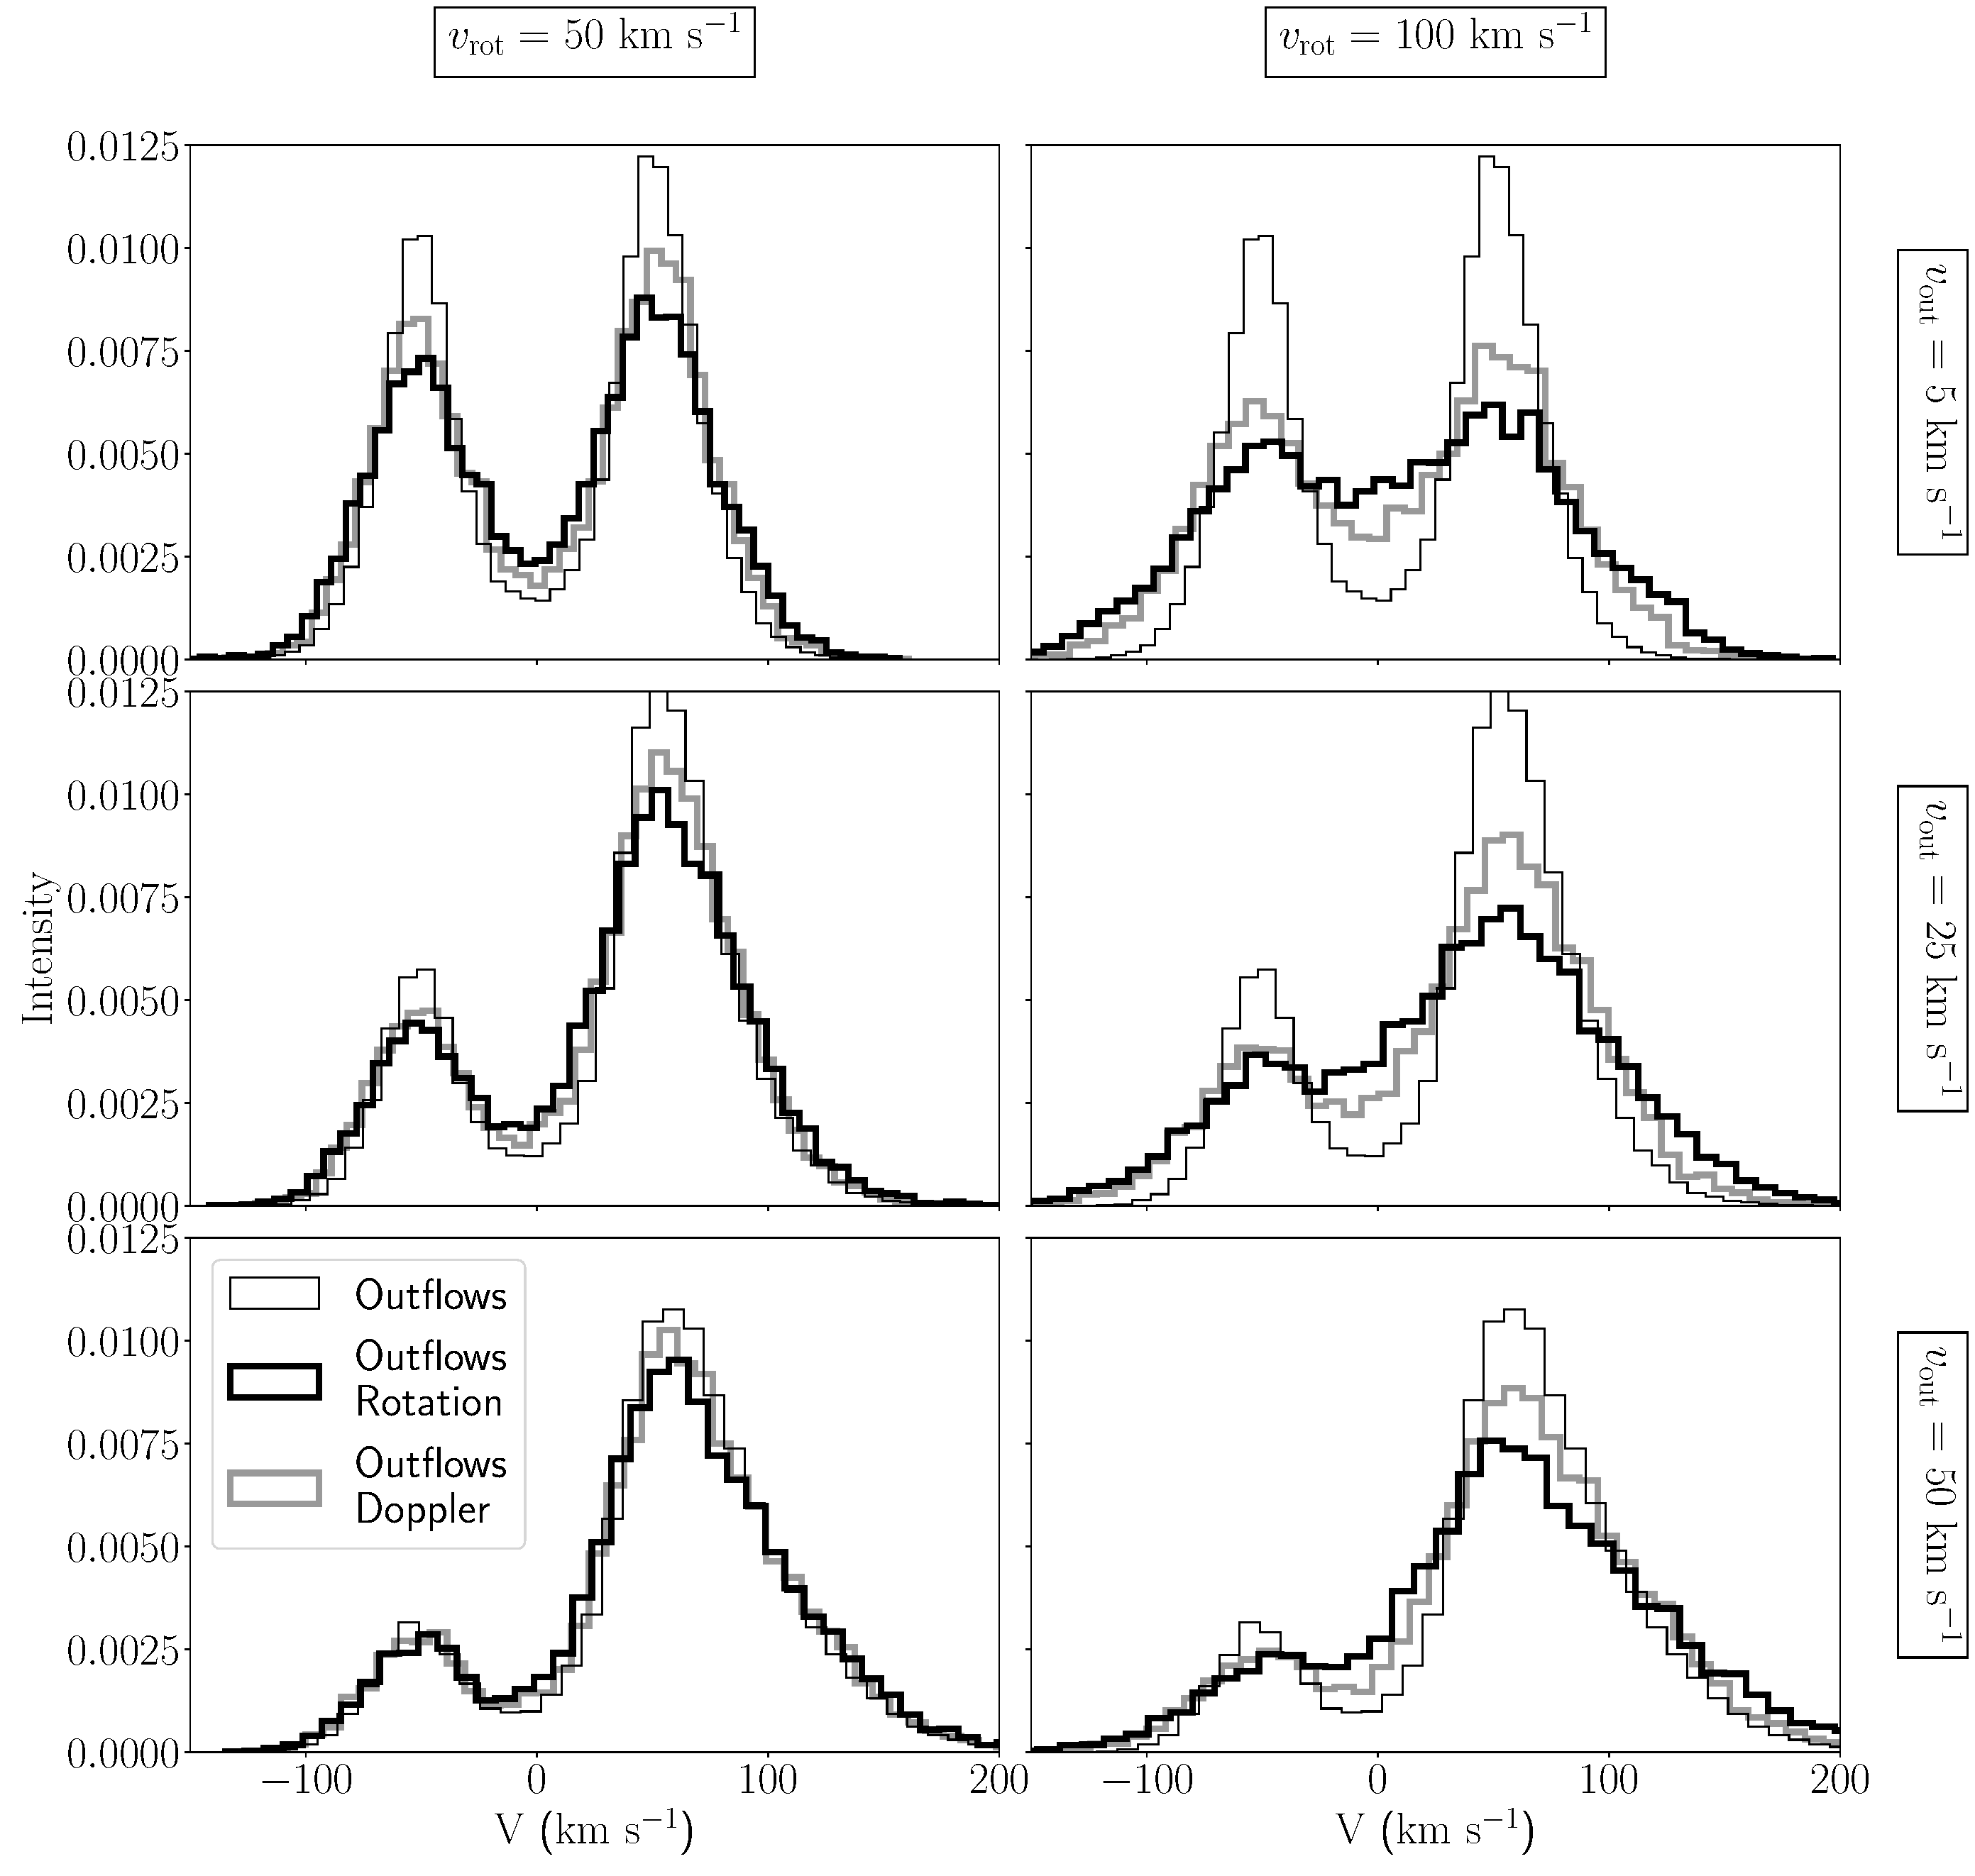
\includegraphics[width=0.49\textwidth]{./figures/results/doppler_shift_logtau5_theta90}
  \end{center}
  \caption{\textbf{Qualitative trends of changing outflow and
      rotational velocity.}
    Same layout as Figure \ref{fig:doppler_shift},
    this time  $\tauh=10^5$ and $\theta=90^\circ$.}
\end{figure}


\begin{figure}
  \begin{center}
    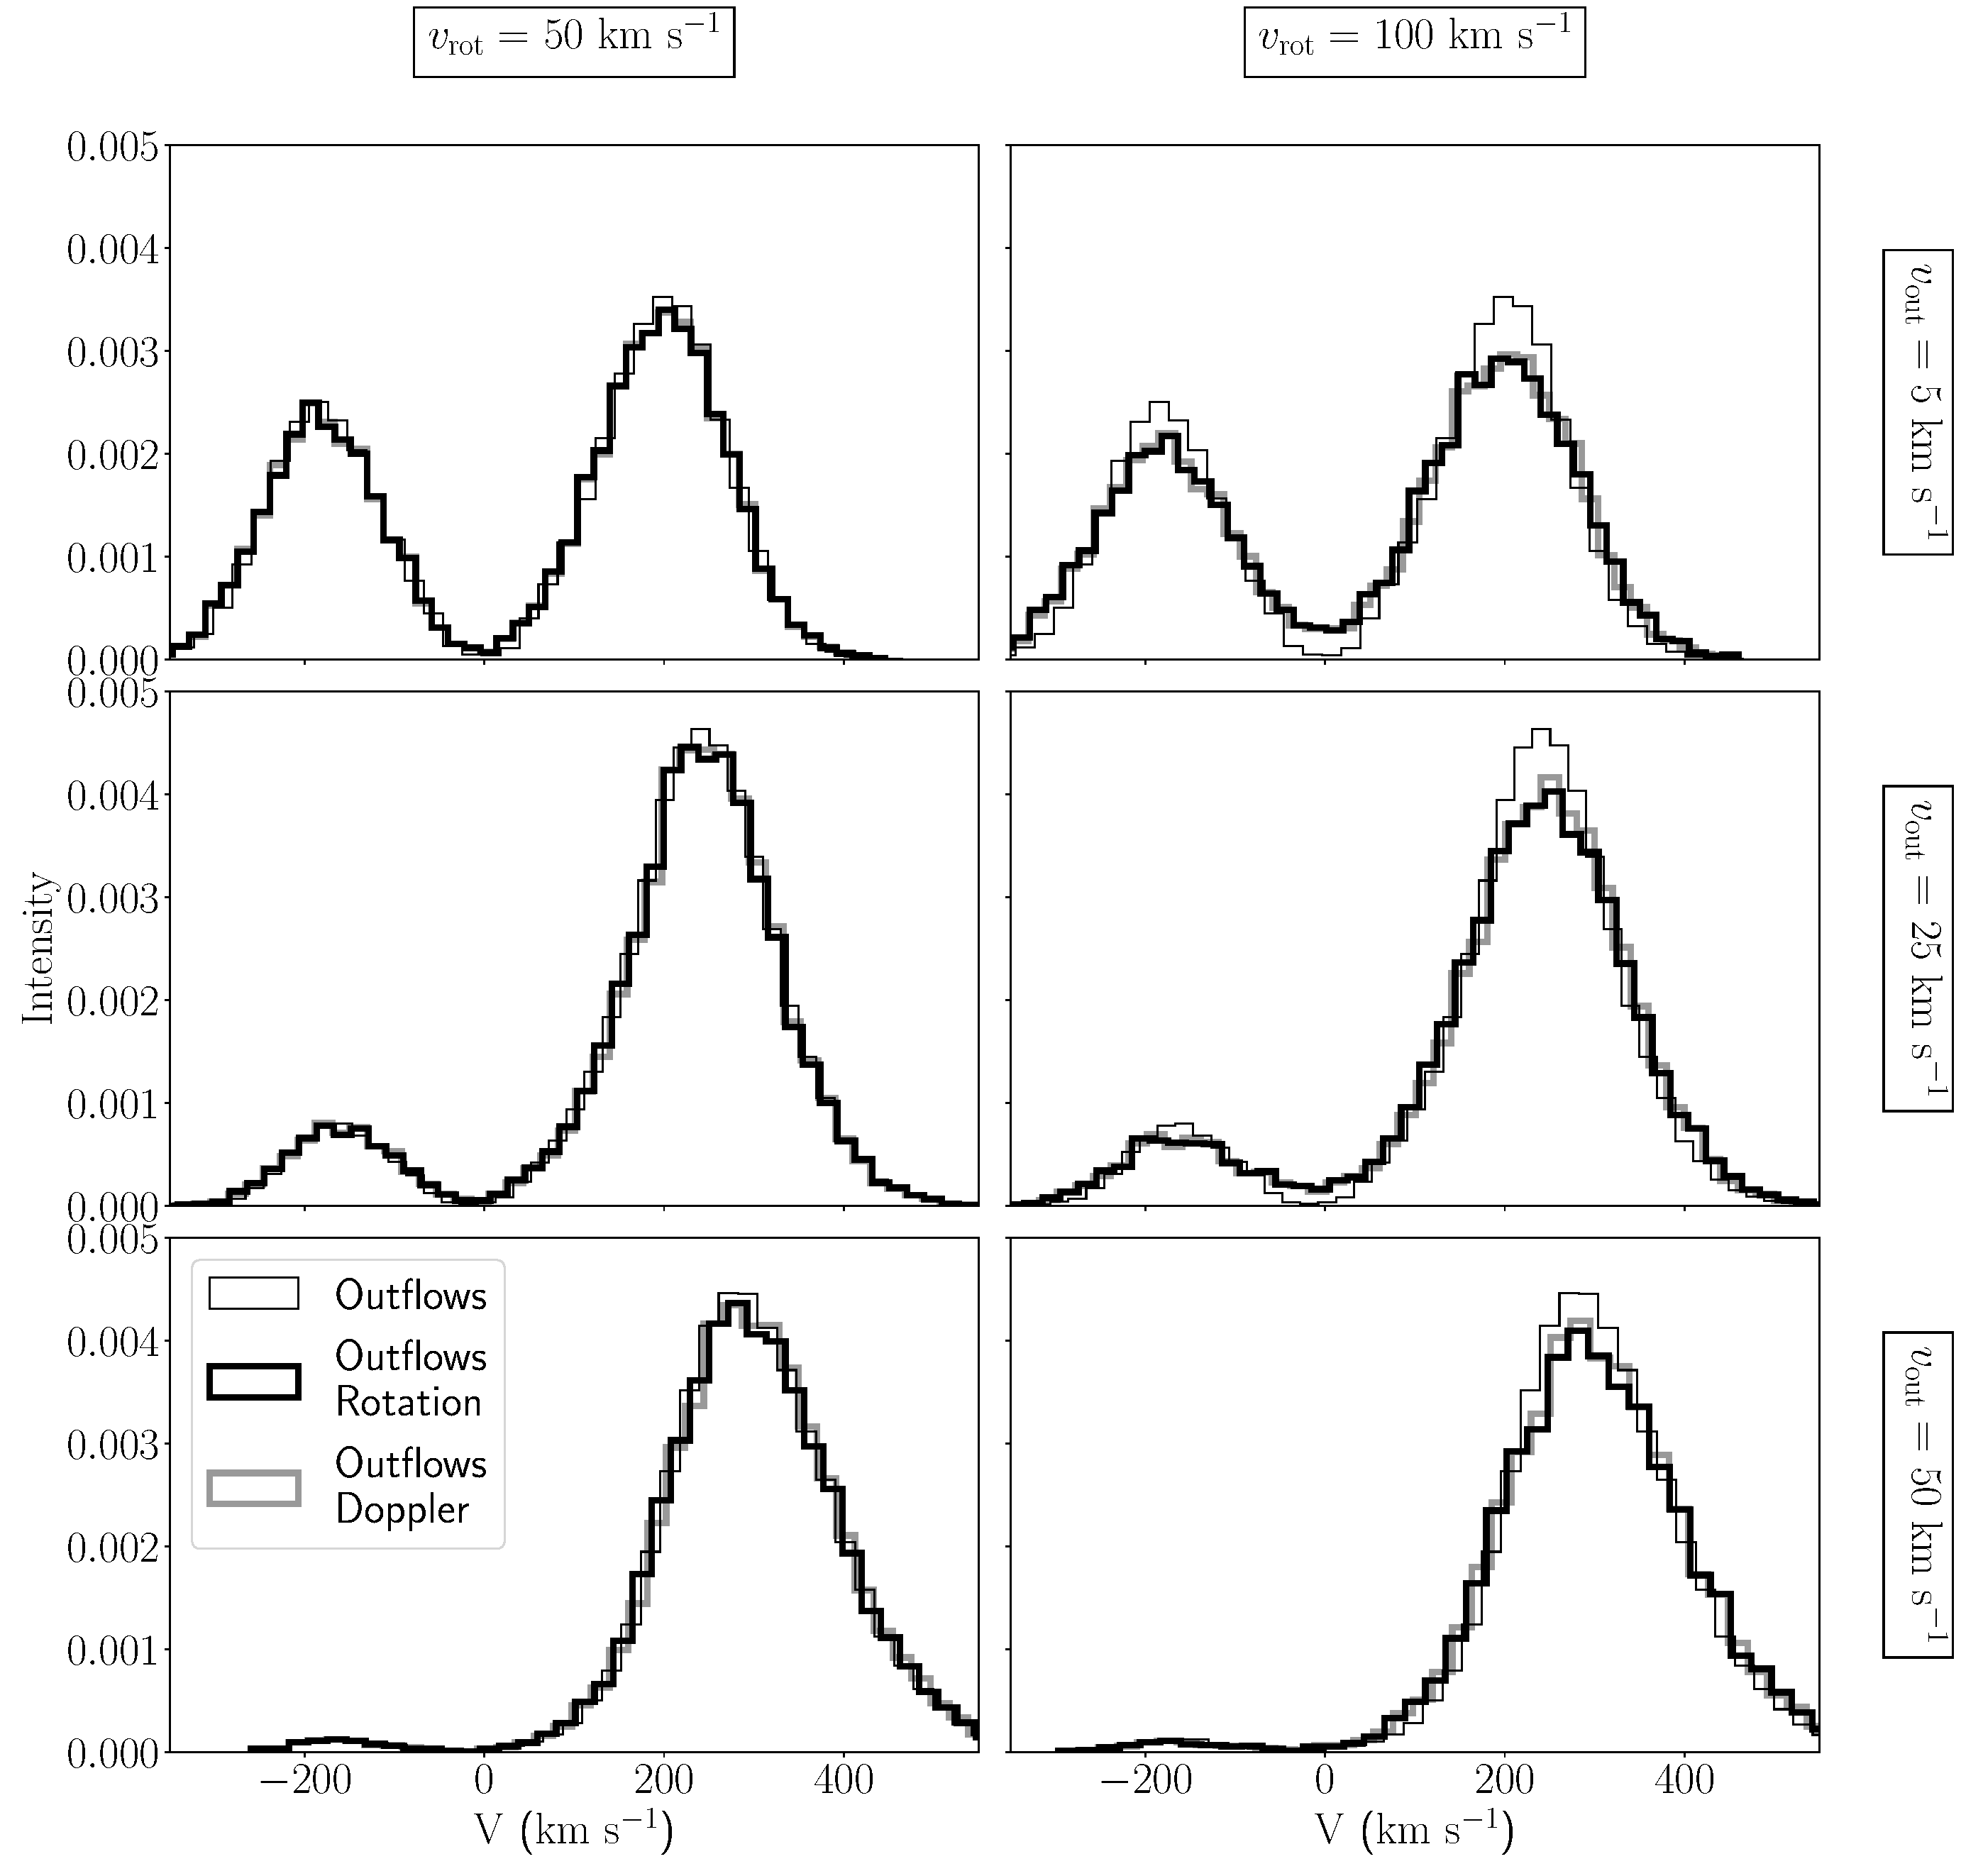
\includegraphics[width=0.49\textwidth]{./figures/results/doppler_shift_logtau7_theta90}
  \end{center}
  \caption{\textbf{Qualitative trends of changing outflow and
      rotational velocity.}
    Same layout as Figure \ref{fig:doppler_shift},
    this time  $\tauh=10^7$ and $\theta=90^\circ$.}
\end{figure}



\end{document}
